\documentclass[b5paper, 12pt, twoside]{report}
\usepackage[utf8]{inputenc}
\usepackage{geometry}
\geometry{
	twoside,
	bindingoffset=7mm,
	verbose,
	marginratio={5:7,5:7},
	textwidth=130mm,
	height=200mm,
	foot=2cm
}
\usepackage[mathscr]{euscript}
\usepackage[protrusion=true, expansion=true]{microtype}
\usepackage[nodisplayskipstretch]{setspace}
\usepackage{tikz}
\usepackage{imakeidx}
\makeindex[columns=2,
title=Index]
\usepackage{graphicx}
\usepackage{caption}
\usepackage{subcaption}
\usepackage{float}
\usepackage{fancyhdr}
\usepackage{fbb}
\usepackage{extarrows}
\usepackage{booktabs}
\usepackage{setspace}
\usepackage{titlesec}
\titlespacing*{\section}{0pt}{1.5ex plus 1ex minus .2ex}{2.3ex plus .2ex}
\titlespacing*{\subsection}{0pt}{1.5ex plus 1ex minus .2ex}{2.3ex plus .2ex}
\usepackage{enumitem}
\setlist[itemize]{noitemsep, topsep=0pt}
\setlist[enumerate]{noitemsep, topsep=0pt}
\usepackage{etoolbox}
\usepackage{amsmath}
\usepackage{amssymb}
\usepackage{breqn}
\usepackage{mathtools}
\usepackage{graphicx}
\usepackage{tocloft}
\usepackage{adjustbox}
\usepackage{tikz-cd}
\usepackage{subcaption}
\captionsetup[subfigure]{labelsep=colon, labelformat=simple, labelfont=sc}
\usepackage[style=nature, sorting=nty]{biblatex}
\addbibresource{main.bib}
\graphicspath{{images/}}
\usepackage{xcolor}
\usetikzlibrary{shapes.geometric, positioning, fit, calc}

\definecolor{darkred}{rgb}{0.7, 0, 0}
\definecolor{azureblue}{rgb}{0, 0.5, 1}
\definecolor{golden}{rgb}{1, 0.8, 0.2}

\newcommand{\R}{{\mathbb{R}}}
\newcommand{\F}{{\mathbb{F}}}
\newcommand{\X}{{\mathcal{X}}}
\newcommand{\V}{{\mathcal{V}}}
\newcommand{\C}{{\mathbb{C}}}
\newcommand{\ima}{\mathrm{im}}
\newcommand{\Hom}{{\mathrm{Hom}}}

\newtheorem{definition}{Definition}[section]
\newtheorem{remark}[definition]{Remark}
\newtheorem{example}[definition]{Example}
\newtheorem{theorem}{Theorem}[section]
\newtheorem{lemma}[theorem]{Lemma}
\newtheorem{proposition}[theorem]{Proposition}
\newtheorem{corollary}[theorem]{Corollary}

\newenvironment{proof}{\paragraph{Proof}}{\hfill$\square$
\vspace{0.5cm}}

\title{Algebraic and Topological Persistence}
\author{Luciano Melodia}
\date{\today}

\begin{document}
	\begin{titlepage}
    \begin{center}
        \vspace*{1cm}
        \Huge
        \textbf{Algebraic and Topological Persistence}
        \vspace{1cm}
        \Large
                
        by\\
        \textbf{Luciano Melodia}
        \vfill
        
\includegraphics[width=8cm]{images/fau.png}
        \vfill
        A bachelor thesis submitted in fulfillment\\
        of the requirements for the degree of\\
        Bachelor of Science (B.Sc.)\\
        in Mathematics\\ 
        \vspace{1.5cm}
        \large
        
\includegraphics[width=8cm]{images/fau.pdf}\\
        \today
    \end{center}
\end{titlepage}
	\begin{center}
    \Large
    \textbf{Algebraic and Topological Persistence}
        
    \vspace{0.4cm}
    \large
    \textbf{Luciano Melodia}
    
    \vspace{0.9cm}
    \textbf{Abstract}
\end{center}

Lorem ipsum dolor sit amet, consectetur adipisicing elit, sed do eiusmod tempor incididunt ut labore et dolore magna aliqua. Ut enim ad minim veniam, quis nostrud exercitation ullamco laboris nisi ut aliquip ex ea commodo consequat. Duis aute irure dolor in reprehenderit in voluptate velit esse cillum dolore eu fugiat nulla pariatur. Excepteur sint occaecat cupidatat non proident, sunt in culpa qui officia deserunt mollit anim id est laborum.

Lorem ipsum dolor sit amet, consectetur adipisicing elit, sed do eiusmod tempor incididunt ut labore et dolore magna aliqua. Ut enim ad minim veniam, quis nostrud exercitation ullamco laboris nisi ut aliquip ex ea commodo consequat. Duis aute irure dolor in reprehenderit in voluptate velit esse cillum dolore eu fugiat nulla pariatur. Excepteur sint occaecat cupidatat non proident, sunt in culpa qui officia deserunt mollit anim id est laborum.

Lorem ipsum dolor sit amet, consectetur adipisicing elit, sed do eiusmod tempor incididunt ut labore et dolore magna aliqua. Ut enim ad minim veniam, quis nostrud exercitation ullamco laboris nisi ut aliquip ex ea commodo consequat. Duis aute irure dolor in reprehenderit in voluptate velit esse cillum dolore eu fugiat nulla pariatur. Excepteur sint occaecat cupidatat non proident, sunt in culpa qui officia deserunt mollit anim id est laborum.
	We begin this work with a brief motivation from an applied context that inspired
	this work. Much of the research in persistence theory has been driven by the
	goal of utilizing persistent homology for data analysis. However, we restrict
	ourselves to providing an illustrative context and then proceed strictly to
	the theory of topological spaces. This thesis addresses the theory of topological
	spaces (\ref{TopologicalSpaces}) and the theoretical foundations of persistence
	theory (\ref{PersistenceTheory}). We discuss chain complexes (\ref{ChainComplex})
	and the associated simplicial homology groups (\ref{SimplicialHomology}), as well
	as their connection to singular homology (\ref{SingularHomology}).
	Additionally, we introduce classical tools of algebraic topology, such as
	exact and short exact sequences (\ref{ExactandShortExactSequences}), and relative
	homology groups obtained by quotienting with subspaces of a topological space (\ref{RelativeHomology}).
	These tools are used to prove the Excision Theorem \ref{ExcisionTheorem} in
	algebraic topology. We then use this theorem to demonstrate the equivalence of
	simplicial and singular homology for triangulable topological spaces, i.e.,
	those topological spaces that admit a simplicial structure (\ref{HomologicalEquivalence}).
	This allows for the use of a more general theory of homology in the investigation
	of topological methods through theoretical considerations.

	In the chapter on homological persistence, we consistently use these tools. We
	develop the theory of persistent homology, the homology of filtrations of
	topological spaces, and the corresponding dual concept of persistent cohomology.
	Finally, we generalize both theories into zigzag persistence. Zigzag modules
	allow for the treatment of maps in both directions along a filtration, making them
	highly useful for local applications of zigzag persistence. This work aims to
	provide mathematicians with a solid foundation for productively engaging with
	the aforementioned theories. Most of the proofs have been rewritten to clarify
	the relationships between the discussed theories. The novelty of this
	contribution lies in the comprehensive presentation of persistence theory and
	its ideas through rigorous mathematical treatment for triangulable topological
	spaces.
	\chapter*{Dedication}

	This thesis is dedicated with deep appreciation to those closest to me, whose
	support was indispensable in writing these pages and undertaking this journey.

	My academic path took me through studies in German and Italian, then to a major
	in Information Science with a focus on Media Informatics, culminating in a
	Master’s degree from Regensburg. A three-year doctoral stint in Computer Science
	at Erlangen followed, after which I shifted my focus to theoretical
	mathematics. Throughout, I grappled with whether I was truly satisfied with my
	choices, always drawn to the underlying structures of language and computing.
	It is with joy that I reflect on these discoveries.

	I am grateful to my mother, Beata, who, despite initial reservations,
	supported my decisions wholeheartedly once they were made.

	A special thanks to my late father, Domenico, who taught me to value the past
	more than the future.

	Thanks also to my sister, Dominique, who never ceased to engage me in
	discussions about physics whenever she had the chance.

	To Luciana, who brought joy and laughter back into my life during challenging times.

	And to all those unnamed, if these words strike a chord, you have touched my life
	in significant ways.

	I have learned much from each of you.

	\chapter*{Declaration}

	I hereby declare that I

	\begin{itemize}
		\item alone wrote the submitted Bachelor's thesis without illicit or improper
			assistance.

		\item did not use any materials other than those listed in the bibliography and
			that all passages taken from these sources in part or in full have been marked
			as citations and their sources cited individually in the thesis. Citations
			include the version (edition and year of publication), the volume and page
			numbers of the cited work.

		\item have not submitted this Bachelor's thesis to another institution and that
			it has never been used for other purposes or to fulfill other requirements,
			in part or in full.
	\end{itemize}

	\vspace{2cm}
	\begin{tabular}{@{}p{3.5in}p{2in}p{2in}@{}}
		\hrulefill                    &  & Erlangen, \today \\
		Luciano Melodia M.A., B.A.    &  &                  \\
		Friedrich-Alexander University \\
		Erlangen-Nürnberg
	\end{tabular}

	\chapter*{Acknowledgements}

	I extend heartfelt thanks to Prof. Dr. Catherine Meusburger, who not only teached
	me the rigors of the Bachelor's program in Mathematics but also illuminated the
	more complex concepts of Linear Algebra I and II. Her invaluable assistance
	during our early sessions, where we dissected exercise sheets in the study room,
	was crucial. I am particularly grateful for the moments she joined us after a refreshing
	cup of coffee, skillfully translating challenging problems into clear
	solutions on the blackboard with swift strokes of chalk.

	My special gratitude is due to my supervisor, Prof. Dr. Kang Li. His readiness
	to engage in discussions was a beacon of motivation, especially when I was lost
	in the dense forest of scientific papers and theorems. Prof. Li's adeptness in
	distilling sprawling research into manageable segments for my bachelor's thesis
	was invaluable, and his excellent guidance has been a cornerstone of my still
	early academic journey in Mathematics.

	Last but not least, I owe a tremendous debt of gratitude to some my friends - Luciana
	Diaconescu, Philipp Gäbelein, Marie-Louise Isenberg, Michael Schleich, Sarah Wiesend,
	Adrian Hieber, Moritz Lanz, Sebastian Müller, Thomas Büttner, Anton Rechenauer,
	Constantin Winkler and Anton Hoof. Their companionship sweetened my days, their
	support was unwavering, and their presence essential to my achievements. Wherever
	they may find themselves now, I wish them every success and hope they know I
	am always here for them.

	\newpage
	\tableofcontents

	\singlespacing
	\chapter{Motivation}
	\pagenumbering{arabic}
	The development of persistence theory\index{persistence theory} in topological data analysis\index{topological data analysis} (TDA) represents a significant advance in the quantitative analysis of complex, high-dimensional data sets. Traditional statistical approaches often fail to capture the intricate geometric and topological structure\index{topological structure}s of such data, especially when they are obscured by noise or nonlinear relationships. Persistence theory, in particular persistent homology\index{persistent homology}\index{homology}, provides a rigorous mathematical framework for the systematic identification and quantification of these topological features at different levels.

Persistent homology\index{homology} is a mathematical concept that analyzes homological features\index{homological features} in data. It uses persistence diagrams\index{persistence diagrams} or barcodes\index{barcodes} to describe the topological structure\index{topological structure} of the data. These representations enable a precise description of the data structure and help to distinguish significant features from noise. The persistent homology\index{persistent homology}\index{homology} techniques are based on algebraic topology\index{algebraic topology}, where homology\index{homology} groups serve as algebraic invariants to classify topological spaces. In persistent homology\index{persistent homology}\index{homology}, this concept is extended to use a filtration where a real-valued function is the parameter of a nested sequence of topological spaces. The features of this filtration are captured in persistence intervals, which indicate the robustness of the features. The persistent homology\index{persistent homology}\index{homology} is realized by constructing simplified complexes from the data by means of efficient computational methods. Persistence diagrams and barcodes\index{barcodes} can not only be descriptive tools, but can also be integrated into statistical and machine learning methods to perform quantitative comparisons between data sets \cite{melodia2018deep,melodia2020persistent,melodia2021estimate,melodia2021homological}.

Persistence theory is a valuable tool in topological data analysis\index{topological data analysis} due to its stability in the face of data perturbations. This theory ensures that small changes in input data only result in minor changes in persistence diagrams\index{persistence diagrams}, confirming the reliability of extracted topological features. This robustness is particularly helpful for analyzing noisy or incomplete data. Persistence theory bridges the gap between abstract mathematical theory and practical data analysis and has become fundamental in this field. It can capture and quantify topological features across scales and demonstrates its importance in modern data science through its broad applicability and robustness. The ongoing development and refinement of this theory are expected to lead to even more powerful tools for analyzing complex data structures and further expanding the scope of topological data analysis\index{topological data analysis}.

\section{History}
The development of persistence theory\index{persistence theory} in TDA has been characterised by the fundamental contributions of pioneering researchers who, together, have established persistence as a central tool for the understanding of the topological structure\index{topological structure} of data.

\paragraph*{Size Theory}
The origins of persistence theory\index{persistence theory} can be traced back to the end of the 20th century, with the work of Patrizio Frosini and Massimo Ferri at the University of Bologna. Their research in set theory focused on the natural pseudodistance between functions defined on homeomorphic topological spaces \cite{Frosini1999,Ferri1998}. Size theory, particularly in its application to $0$-dimensional homology\index{homology}, provided a framework for quantifying differences between shapes and topological spaces, introducing a method to capture persisting features across scales.

\paragraph*{Fractal Geometry}
Vanessa Robins extended the application of persistence theory\index{persistence theory} to fractal geometry during her doctoral research at the University of Colorado Boulder. Using alpha forms -- a concept introduced by Herbert Edelsbrunner and colleagues -- Robins demonstrated the utility of persistent homology\index{persistent homology}\index{homology} in capturing the multiscale structure of fractal sets \cite{Robins2000, Edelsbrunner1994}.

\paragraph*{Algebraic Foundations}
Herbert Edelsbrunner and his team at Duke University made significant progress in formalising the algebra of persistence theory\index{persistence theory} \cite{Edelsbrunner2000}. They introduced key concepts such as simplicial filtrations, which systematically construct topological spaces from data points by adding simplices in a hierarchical fashion. This filtration process tracks topological features -- such as connected components, loops and voids -- across different scales, leading to the birth and death of these features. The distinction between positive and negative simplices, introduced by Edelsbrunner's group, is crucial for understanding the emergence and decay of homological features\index{homological features} within a point cloud. 

\section{Computational Aspects}
The computational efficiency of persistence theory\index{persistence theory} has been crucial to its widespread adoption in various scientific domains. This efficiency, based on robust algorithmic foundations, has established persistence theory\index{persistence theory} as an essential tool for analysing complex datasets.

\paragraph*{Algorithmic Developments}
The algorithms for computing persistent homology\index{persistent homology}\index{homology}, developed by Herbert Edelsbrunner and colleagues, are founded upon rigorous mathematical theory and optimized for practical application. These algorithms entail the construction and reduction of boundary matrices for the efficient computation of homology\index{homology} groups across a filtration of simplicial complex\index{simplicial complex}es. Among these algorithms, the matrix reduction algorithm plays a pivotal role in the computation of persistence intervals. The practical implementation of these algorithms has led to the development of standard software packages, including GUDHI, Ripser, and Dionysus \cite{Otter2017}.

\paragraph*{Applications in Life Sciences}
In the field of life sciences, persistent homology\index{persistent homology}\index{homology} has emerged as a powerful tool for the study of the structure and function of biological molecules, particularly proteins. Proteins are complex macromolecules whose function is intricately linked to their three-dimensional structure. Persistent homology\index{homology} is a method for identifying patterns, within a protein's structure that persist across different scales. These patterns frequently correspond to critical functional sites, such as binding pockets or active sites, and provide insights into protein interactions and stability under diverse conditions \cite{Kovacev-Nikolic2016}. In the field of neuroscience, persistence theory\index{persistence theory} has been employed to examine brain networks, providing a novel methodology for analysing the intricate connectivity patterns that underpin brain function. By constructing simplicial complex\index{simplicial complex}es from neural data, researchers employ persistent homology\index{persistent homology}\index{homology} to monitor alterations in brain region connectivity over time. This approach has yielded new insights into the manner in which brain networks reorganise during cognitive processes or in response to neurological diseases \cite{Giusti2016}. In the field of machine learning, persistent homology\index{persistent homology}\index{homology} is a valuable tool for uncovering the underlying topological structure\index{topological structure} of data distributions. This enables the effective performance of tasks such as clustering, classification, and anomaly detection. The topological features of data provide crucial insights into the organisation of the data space. For instance, persistent homology\index{persistent homology}\index{homology} can detect clusters of data points that form distinct topological features, such as loops or voids, which correspond to different classes or subpopulations within the data \cite{Hofer2017,melodia2018deep,melodia2020persistent,melodia2021estimate,melodia2021homological}. The integration of topological information into machine learning models enhances their robustness and generalisation, particularly in the presence of noise or incomplete data.

\paragraph*{Robustness to Noise}
A defining feature of persistence theory\index{persistence theory} is its resilience to noise, which represents a substantial advantage in the context of real-world data analysis. Persistence theory is concerned with the topological features that remain consistent across different scales, thereby filtering out noise-induced artefacts. This robustness is mathematically grounded in stability theorems, which guarantee that minor changes are induced in the persistence diagram by small perturbations in the input data \cite{Cohen-Steiner2007}.

\section{Advanced Extensions}
The adaptability and extensibility of persistence theory\index{persistence theory} are exemplified by its sophisticated developments, which expand its applicability to more intricate mathematical and data analysis problems. Among these extensions, discrete Morse theory, multiparameter persistence, and zigzag persistence represent notable advancements, each addressing particular challenges and broadening the scope of TDA.

\paragraph*{Discrete Morse Theory}
The discrete Morse theory, as first proposed by Robin Forman, represents an extension of the classical Morse theory to discrete spaces, such as simplicial complex\index{simplicial complex}es. This extension is of particular value in TDA, as it facilitates the simplification of complex spaces while ensuring the preservation of essential topological characteristics. The construction of discrete Morse functions on simplicial complex\index{simplicial complex}es allows for the reduction of the number of critical simplices, thereby facilitating more efficient persistent homology\index{persistent homology}\index{homology} computations \cite{Forman2002}. The critical simplices correspond to significant topological features, and focusing on these reduces the computational complexity of calculating persistence intervals. This approach is especially advantageous in large datasets, where the number of simplices can render traditional homology\index{homology} computations impractical.

\paragraph*{Multiparameter Persistence}
Multiparameter persistence represents an extension of the traditional single-parameter filtration approach, whereby filtrations are considered that are indexed by multiple parameters simultaneously. This enables a more comprehensive examination of topological characteristics, as distinct parameters facilitate the capture of diverse aspects of the data's structural elements. To illustrate, one might filter a dataset by both scale and density, thereby uncovering topological features that would otherwise remain invisible under a $1$-parameter filtration \cite{CarlssonZomorodian2009}. The employment of multiple parameters gives rise to a more intricate algebraic structure, thereby presenting computational and visualisation challenges associated with multiparameter persistence modules. In contrast to single-parameter persistence, where persistence diagrams\index{persistence diagrams} or barcodes\index{barcodes} offer a comprehensive invariant, multiparameter persistence lacks a straightforward representation. Instead, more complex invariants, such as generalized persistence diagrams\index{persistence diagrams} or rank invariants, capture the intricate relationships between parameters.

\paragraph*{Zigzag Persistence}
Zigzag persistence represents an extension of the traditional persistent homology\index{persistent homology}\index{homology} framework to accommodate dynamic datasets, wherein the data may undergo change over time or under varying conditions. In contrast to the standard persistence approach, which necessitates a monotonically increasing sequence of spaces, zigzag persistence permits both forward and backward inclusions throughout the filtration \cite{Carlsson2010}. This flexibility allows for the analysis of topological features in settings where data is not static, such as time-varying networks or datasets undergoing changes due to external factors. Zigzag persistence captures the evolution of topological features, including their appearance, disappearance, and reappearance as the data changes, providing a more accurate and comprehensive analysis of dynamic systems. The algebraic structure underlying zigzag persistence is more intricate than that of standard persistence, involving directed graphs and more complex homological algebra.

\section{Our Contribution}
This work presents a comprehensive summary of persistent homology\index{persistent homology}\index{homology} theory, unifying various proofs to facilitate a unified examination of persistence modules, persistent (co)homology\index{homology}, and zigzag persistence from an algebraic-topological perspective.The objective of this study is to provide a mathematically precise explanation for the remarkable success of persistent homology\index{persistent homology}\index{homology} in data analytics. Our approach is based on the assumption that real-world data resides on a triangulable topological space and that simplicial structures allow us to derive invariants of this space. We rigorously prove the validity of this approach and demonstrate that it is well-defined. Furthermore, we elucidate the interaction between cohomology\index{homology} and zigzag persistence on persistence intervals, addressing and resolving non-trivial gaps previously left open in the literature.

	\chapter{Topological Spaces and Groups}
	Topological persistence is deeply rooted in algebraic topology, which studies topological
spaces and functions based on algebraic objects and their properties. An example
of this are homotopy and homology theories, which are essential for understanding
the construction and connectedness of surfaces, a central aspect of data
analysis. Persistent homology, the central tool of topological persistence, extends
classical homology to identify features across multiple scales. Introduced by
Edelsbrunner et al. in their seminal paper \cite{edelsbrunner2000triangulations},
persistent homology examines multi-scale topological features through a
filtration process - an indexed family of nested spaces that starts with the
empty set and progressively covers the entire space under study. Each stage of filtration
represents a snapshot of the topological space at a different resolution and captures
the appearance and disappearance of homology groups in different dimensions that
encode topological properties such as connected components, holes and voids.

Mathematically, the persistence of homological features is visualized with the help
of diagrams or barcode representations. These visual aids represent the
emergence (birth) and vanishing (death) of topological features when the filter
parameter changes. The duration of a feature's presence, represented by the
length of its interval in the diagram, indicates its significance, with longer
intervals suggesting features that represent the underlying data's likely true
characteristics rather than mere noise. The robustness of persistent homology,
in particular its resistance to minor perturbations in the data, is captured in the
Stability Theorem \ref{stability}. This theorem, proved by Cohen-Steiner, Edelsbrunner and Harer
\cite{bendich2007inferring}, states that slight variations in the input data lead
to slight changes in the persistence barcodes. This property is crucial for
practical applications as it guarantees that the topological summaries are both
reliable and meaningful for the actual underlying structures.

We start with basic concepts such as topological spaces and groups, which are crucial
for understanding and encoding connectedness and other invariants. The
discussion extends to simplicial complexes, which are essential for modeling data
structures in topological data analysis. We explore simplicial and singular
homology groups to accurately quantify topological features, and dwell on singular
chain complexes and exact sequences to deepen the algebraic aspects of persistence theory. This will be useful in some of the later proofs when we discuss the algebraic
nature of the persistence module.


\section{Simplicial Complexes}
\label{Simplicial Complexes} We note that a set of points
$X = \{x_{0}, x_{1}, \ldots, x_{d}\}$ in $\mathbb{R}^{n}$ is affinely
independent\index{affinely independent} if no affine subspace\index{affine
subspace}
of dimension less than $d$ contains all the points in $X$. Such a set of points is
commonly called point cloud.

\begin{definition}[$d$-Simplex]{\cite[\S 2.1]{boissonnat2018geometric}}
\label{d-simplex} A $d$-dimensional
	simplex $\sigma^{(d)}$, or $d$-simplex\index{$d$-simplex}, is the set of all convex combinations
	of a set $X = \{x_{0}, x_{1}, \ldots, x_{d}\} \subset \mathbb{R}^{n}$, where
	$X$ consists of $d+1$ affinely independent points.
	
	Formally, $\sigma^{(d)}$ is
	defined by:
	\begin{equation}
		\sigma^{(d)}:= \left\{\sum_{i=0}^{d}\lambda_{i} x_{i} \; | \; \sum_{i=0}^{d}\lambda
		_{i} = 1, \; \lambda_{i} \geq 0\right\}.
	\end{equation}
\end{definition}

As a convention, the empty set $\emptyset$ is considered a face\index{face}, corresponding
to the simplex formed by the empty subset of vertices. Specifically, a $0$-simplex
corresponds to a single point, a $1$-simplex to a line segment between two
points, a $2$-simplex to a triangle, and a $3$-simplex to a tetrahedron. Notably,
a $d$-simplex is homeomorphic to the $d$-dimensional disk $D^{d}$.

\begin{theorem}[$d$-Disk to $d$-Simplex]
	The $d$-simplex $\sigma^{(d)}$ is homeomorphic to the $d$-dimensional disk $D^{d}$.
\end{theorem}

\begin{proof}
Define the standard \( d \)-simplex \( \sigma^{(d)} \) as
\begin{align}
\sigma^{(d)} := \left\{(x_{0}, \ldots, x_{d}) \in \mathbb{R}^{d+1} \mid \sum_{i=0}^{d} x_{i} = 1, \, x_{i} \geq 0\right\},
\end{align}
and the \( d \)-dimensional disk \( D^{d} \) as
\begin{align}
D^{d} := \left\{(x_{0}, \ldots, x_{d-1}) \in \mathbb{R}^{d} \mid \sum_{i=0}^{d-1} x_{i}^{2} \leq 1\right\}.
\end{align}

We construct a homeomorphism \( f: \sigma^{(d)} \rightarrow D^{d} \) by
\begin{align}
f(x_{0}, \ldots, x_{d}) = (\sqrt{x_{0}}, \ldots, \sqrt{x_{d-1}}),
\end{align}
where \( x_{d} = 1 - \sum_{i=0}^{d-1} x_{i} \). This map is well-defined since
\begin{align}
\sum_{i=0}^{d-1} (\sqrt{x_{i}})^{2} = \sum_{i=0}^{d-1} x_{i} \leq 1.
\end{align}

The inverse \( g: D^{d} \rightarrow \sigma^{(d)} \) is given by
\begin{align}
g(y_{0}, \ldots, y_{d-1}) = (y_{0}^{2}, \ldots, y_{d-1}^{2}, 1 - \sum_{i=0}^{d-1} y_{i}^{2}),
\end{align}
ensuring that \( g \) is well-defined because \( \sum_{i=0}^{d-1} y_{i}^{2} \leq 1 \) implies
\( 1 - \sum_{i=0}^{d-1} y_{i}^{2} \geq 0 \). Both \( f \) and \( g \) are continuous and are inverses of each other, as shown by
\( f(g(y)) = y \) for all \( y \in D^{d} \) and \( g(f(x)) = x \) for all
\( x \in \sigma^{(d)} \).
\end{proof}

Furthermore, it is important to note that $\sigma^{(d)}$ represents the convex hull\index{convex
hull}
of the points $X = \{x_{0}, x_{1}, \ldots, x_{d}\}$, defined as the smallest convex
subset of $\mathbb{R}^{n}$ that contains all of these points. The faces of the
simplex $\sigma^{(d)}$, with vertex set $X$, are formed by the simplices
corresponding to subsets of $X$. A $d$-face of a simplex consists of a subset of
the vertices with cardinality $d+1$. The faces of a $d$-simplex with dimensions
less than $d$ are known as its proper faces\index{proper faces}. Two simplices
are considered properly situated\index{properly situated} if their intersection is
either empty or a face of both simplices. By identifying simplices along entire
faces, we can construct the corresponding simplicial complexes\index{simplicial
complex}.

\begin{definition}
	[Simplicial Complex]{\cite[\S 2.2]{boissonnat2018geometric}} \label{simplicialcomplex}
	A simplicial complex $K$ is a finite collection of simplices that satisfies the
	following properties:
	\begin{enumerate}
		\item For every simplex $\sigma^{(d)}$ in $K$, and every face $\tau^{(k)}$
			of $\sigma^{(d)}$ with $k < d$, it follows that $\tau^{(k)}$ is also in $K$.

		\item Any two simplices $\sigma^{(d)}$ and $\tau^{(k)}$ in $K$ are properly situated;
			that is, their intersection is either empty or a face of both simplices.
	\end{enumerate}
\end{definition}

The dimension of a simplicial complex $K$ is defined as the highest dimension among
its simplices. For a simplicial complex $K$ in $\mathbb{R}^{n}$, the underlying space
$\vert K \vert$ is the union of all the simplices in $K$. The topology of $K$ is
determined by the topology induced on $\vert K \vert$ by $\mathbb{R}^{n}$'s
standard topology. Notably, when the vertex set is specified, a simplicial complex
in $\mathbb{R}^{n}$ can be fully characterized by listing its simplices. Thus, it
can be described purely in terms of combinatorics using abstract simplicial complexes.

\begin{definition}
	[Abstract Simplicial Complex]{\cite[\S 2.3]{boissonnat2018geometric}} \label{abstractsimplicialcomplex}
	Consider a finite set $V = \{v_{0}, \ldots, v_{d}\}$. An abstract simplicial
	complex\index{abstract simplicial complex} $\tilde{K}$ with vertex set $V$ is a
	collection of finite subsets of $V$ that satisfies the following conditions:
	\begin{enumerate}
		\item Every singleton set $\{v_{i}\}$, where $v_{i} \in V$, is included in $\tilde
			{K}$.

		\item If a set $\sigma^{(d)}$ is in $\tilde{K}$ and $\tau^{(k)}$ is a subset
			of $\sigma^{(d)}$, then $\tau^{(k)}$ must also be in $\tilde{K}$.
	\end{enumerate}
\end{definition}

The abstract simplicial complex $\tilde{K}$ associated with a simplicial complex
$K$ is commonly referred to as its vertex scheme\index{vertex scheme}.
Conversely, if an abstract complex $\tilde{K}$ serves as the vertex scheme for a
complex $K$ in $\mathbb{R}^{n}$, then $K$ is known as a geometric realization\index{geometric
realization} of $\tilde{K}$.

\begin{proposition}
	Every finite abstract simplicial complex $\tilde{K}$ can be geometrically realized
	in Euclidean space.
\end{proposition}

\begin{proof}
	Let $\{v_{0}, v_{1}, \ldots, v_{d}\}$ denote the vertex set of $\tilde{K}$,
	with $0 \leq d < n$ representing the number of vertices in $\tilde{K}$. Consider $\sigma^{(d-1)}
	\subset \mathbb{R}^{n}$, the simplex formed by the span of
	$\{e_{1}, e_{2}, \ldots, e_{d}\}$, where $e_{i}$ represents the $i$-th unit vector.
	In this context, $K$ refers to the subcomplex of $\sigma^{(d-1)}$ such that $[e
	_{i_0}, \ldots, e_{i_l}]$ is a $l$-simplex of $K$ with $0 \leq l \leq d$ if and only if $[v_{i_0}, \ldots
	, v_{i_l}]$ is a simplex of $\tilde{K}$.
\end{proof}

Pay attention, that this result is in particular interesting for data analysis, as computer aided methods deal with finite point sets. All realizations of an abstract simplicial complex are homeomorphic to each other.
The specific realization mentioned above is referred to as the natural
realization\index{natural realization}.

\begin{proposition}[Equivalence of Geometric Realizations]
	Let $\tilde{K}$ be an abstract simplicial complex. Then any two geometric
	realizations $|\tilde{K}|_{1}$ and $|\tilde{K}|_{2}$ of $\tilde{K}$ are
	homeomorphic.
\end{proposition}

\begin{proof}
	Consider two geometric realizations $|\tilde{K}|_{1}$ and $|\tilde{K}|_{2}$ of
	the abstract simplicial complex $\tilde{K}$. Each realization
	$|\tilde{K}|_{i}$ is constructed by mapping the vertices of $\tilde{K}$ to
	points in $\mathbb{R}^{d}$, and by identifying each simplex in $\tilde{K}$ with
	the convex hull of its image under this mapping. By construction, each simplex
	in $|\tilde{K}|_{i}$ corresponds homeomorphically to a standard $l$-simplex in
	$\mathbb{R}^{d}$ for the appropriate $l$ for integers $0 \leq l \leq d$.

	To establish a homeomorphism between $|\tilde{K}|_{1}$ and $|\tilde{K}|_{2}$,
	define a map $f: |\tilde{K}|_{1} \to |\tilde{K}|_{2}$ that acts on each vertex
	$v$ of $\tilde{K}$ by mapping it from its image in $|\tilde{K}|_{1}$ to its
	image in $|\tilde{K}|_{2}$. Extend $f$ linearly to each simplex in $|\tilde{K}|
	_{1}$, where a simplex is represented as a convex combination of the images of
	its vertices. Given the two geometric realizations $|\tilde{K}|_{1}$ and $|\tilde{K}|_{2}$
	of $\tilde{K}$, where vertices $v_{i}$ in $|\tilde{K}|_{1}$ are mapped to points
	$p_{i}$ in $\mathbb{R}^{d}$ and in $|\tilde{K}|_{2}$ to points $q_{i}$, the
	map $f: |\tilde{K}|_{1} \to |\tilde{K}|_{2}$ is defined such that for each
	vertex $v_{i}$, corresponding to $p_{i}$ in $|\tilde{K}|_{1}$, we set
	$f(p_{i}) = q_{i}$. This map is linearly extended across each simplex in $|\tilde
	{K}|_{1}$.

	Specifically, for a point $x$ and an integer $0 \leq k \leq d$ within a simplex of $|\tilde{K}|_{1}$, expressed
	as a convex combination $x = \sum_{j=1}^{k}\lambda_{j} p_{i_j}$,
	where $\{v_{i_1}, v_{i_2}, \ldots, v_{i_k}\}$ denote the vertices of the simplex
	and $\lambda_{j} \geq 0$ with $\sum_{j=1}^{k}\lambda_{j} = 1$, the function
	$f$ is defined by $f(x) = \sum_{j=1}^{k}\lambda_{j} q_{i_j}$.
	
	This ensures that $f$ is a continuous and bijective map, preserving
	the simplicial structure and thereby establishing $f$ as a homeomorphism between
	$|\tilde{K}|_{1}$ and $|\tilde{K}|_{2}$. $f$ is continuous on each simplex because it represents a linear transformation
	on compact convex subsets in $\mathbb{R}^{d}$. Since both $|\tilde{K}|_{1}$
	and $|\tilde{K}|_{2}$ are topologized by the quotient of their respective
	disjoint unions of simplices under an equivalence relation that glues them
	along common faces, and since $f$ preserves these gluing conditions, $f$ is
	continuous globally. Each simplex and its face structure in $|\tilde{K}|_{1}$ maps
	uniquely onto a corresponding simplex and face structure in $|\tilde{K}|_{2}$,
	rendering $f$ bijective.

	Similarly, the inverse map $g: |\tilde{K}|_{2} \to |\tilde{K}|_{1}$ can be constructed
	by reversing the roles of $|\tilde{K}|_{1}$ and $|\tilde{K}|_{2}$. It also
	maintains continuity for analogous reasons to $f$.

	Thus, $|\tilde{K}|_{1}$ and $|\tilde{K}|_{2}$ are homeomorphic.
\end{proof}

Furthermore, it has been proven that any finite abstract simplicial complex of dimension
$d$ can be realized as a simplicial complex in $\mathbb{R}^{2d+1}$.

\begin{theorem}[Realizations into $\mathbb{R}^{2d+1}$]
	Any finite abstract simplicial complex of dimension $d$ can be realized as a simplicial
	complex in $\mathbb{R}^{2d+1}$.
\end{theorem}

\begin{proof}
	Let $\tilde{K}$ be a finite abstract simplicial complex of dimension $d$. We
	will construct an injective geometric realization
	$f: \tilde{K}\to \mathbb{R}^{2d+1}$.

	First, define an injective map $\tilde{f}: V(\tilde{K}) \to \mathbb{R}^{2d+1}$
	for the vertex set $V(\tilde{K})$ of $\tilde{K}$. Since $V(\tilde{K})$ is
	finite and $\mathbb{R}^{2d+1}$ has sufficient dimensionality, injectivity is guaranteed.
	Adjust $\tilde{f}$ if necessary to ensure the images of the vertices of each
	simplex $\sigma \in \tilde{K}$ are affinely independent. This can be achieved by
	slight perturbations within $\mathbb{R}^{2d+1}$, leveraging the ample
	dimensionality to avoid overlaps. We extend $\tilde{f}$ to a map $f: \tilde{K}\to \mathbb{R}^{2d+1}$ by defining
	it on each simplex $\sigma = [v_{0}, \ldots, v_{k}]$ through the unique affine
	map $v_{i} \mapsto \tilde{f}(v_{i})$. The injective and affine properties of $\tilde
	{f}$ on vertices guarantee that $f$ is injective over each simplex and preserves
	the simplicial structure. Specifically, for any simplices $\sigma, \tau \in \tilde
	{K}$, we have:
	\begin{align}
		f(|\sigma| \cap |\tau|) = f(|\sigma|) \cap f(|\tau|).
	\end{align}

	Thus, $f$ provides an injective geometric realization of $\tilde{K}$ as a simplicial
	complex in $\mathbb{R}^{2d+1}$.
\end{proof}

\section{Simplicial Homology}
\label{Simplicial Homology}
Given a set \( V \) representing the vertices of a \( d \)-simplex
\( \sigma^{(d)} \), we can establish an orientation for the simplex by selecting a
specific ordering of the vertices. If the vertex ordering differs from our chosen
order by an odd permutation, the orientation is considered reversed, while even permutations
preserve the orientation. Thus, a simplex can have only two possible orientations.
Moreover, the orientation of a \( d \)-simplex induces an orientation on its \( (d-1) \)-faces.
Specifically, if \( \sigma^{(d)} := (v_{0}, v_{1}, \ldots, v_{d}) \) represents an oriented
\( d \)-simplex, then the orientation of the \( (d-1) \)-face \( \tau^{(d-1)} \) of
\( \sigma^{(d)} \), omitting the vertex \( v_{i} \), is given by
\begin{equation}
\tau_{i}^{(d-1)} = (-1)^{i} (v_{0}, \ldots, v_{i-1}, v_{i+1}, \ldots, v_{d}).
\end{equation}

\begin{definition}[$d$-Chain]{\cite[\S 2.3]{zomorodian2004computing}}
\label{d-Chain}
Given a set \(\{\sigma_{1}^{(d)}, \ldots, \sigma_{k}^{(d)}\}\) of arbitrarily oriented \(d\)-simplices in a complex \(K\) and an abelian group \(G\), a \(d\)-chain \(c\) with coefficients \(g_{i} \in G\) is defined as a formal sum:
\begin{align}
c := g_{0}\sigma^{(d)}_{0} + g_{1}\sigma^{(d)}_{1} + \ldots + g_{k}\sigma^{(d)}_{k} = \sum_{i=0}^{k} g_{i}\sigma^{(d)}_{i}.
\end{align}
\end{definition}

Henceforth, we will assume that \( G = (\mathbb{Z}, +) \).

\begin{lemma}
The set of simplicial \( d \)-chains \( C^{\Delta}_{d} \) forms an abelian group \( (C^{\Delta}_{d}, +) \).
\end{lemma}

\begin{proof}
The identity element of the group is the empty chain, given by:
\begin{align}
e_{C^{\Delta}_d} = \sum_{i \in \emptyset} g_{i} \sigma_{i}^{(d)} = e_{G} = 0.
\end{align}

The sum of two chains is defined as:
\begin{align}
c + c' = \sum_{i=0}^{k} g_{i} \sigma_{i}^{(d)} + \sum_{j=1}^{l} g'_{j} \sigma_{j}^{(d)},
\end{align}
which simplifies to:
\begin{align}
c + c' = \sum_{i=0}^{\min(k, l)} (g_{i} + g'_{i}) \sigma_{i}^{(d)} + 
\begin{cases}
\sum_{j=\min(k, l)+1}^{\max(k, l)} g_{j} \sigma_{j}^{(d)} & \text{if } k > l, \\
0 & \text{if } k = l, \\
\sum_{j=\min(k, l)+1}^{\max(k, l)} g'_{j} \sigma_{j}^{(d)} & \text{if } k < l.
\end{cases}
\end{align}
Hence, \( c + c' \in C^{\Delta}_{d} \).

The associativity of the group operation in \( C^{\Delta}_{d} \) follows directly from
the associativity of the group operation in \( G \).

The inverse element is given by:
\begin{align}
c + (-c) = \sum_{i=0}^{k} g_{i} \sigma_{i}^{(d)} + \sum_{i=0}^{k} (-g_{i}) \sigma_{i}^{(d)} = \sum_{i=0}^{k} (g_{i} - g_{i}) \sigma_{i}^{(d)} = e_{C^{\Delta}_d}.
\end{align}
Thus, \( (C^{\Delta}_{d}, +) \) is an abelian group.
\end{proof}

\begin{definition}[Boundary]{\cite[p.106]{hatcher2005algebraic}} 
Let \( \sigma^{(d)} \) be an oriented \( d \)-simplex in a complex \( K \). The boundary of \( \sigma^{(d)} \) is defined as the simplicial \( (d-1) \)-chain of \( K \) with coefficients in the abelian group \( G \), given by
\begin{align}
\partial(\sigma^{(d)}) = \sum_{i=0}^{d} (-1)^{i} \sigma^{(d-1)}_{i},
\end{align}
where \( \sigma^{(d-1)}_{i} \) is a \( (d-1) \)-face of \( \sigma^{(d)} \). If \( d = 0 \), we define \( \partial(\sigma^{(0)}) = 0 \).
\end{definition}

Since \( \sigma^{(d)} \) is an oriented simplex, the \( \sigma^{(d-1)}_{i} \) faces also have associated orientations. We extend the definition of the boundary linearly to elements of \( C^{\Delta}_{d} \).

\begin{lemma}
	The boundary operator is a group homomorphism
	\begin{align}
		\partial: C^{\Delta}_{d} \to C^{\Delta}_{d-1}.
	\end{align}
\end{lemma}

\begin{proof}
We define the boundary operator for a \( d \)-chain \( c = \sum_{i=0}^{k} g_{i} \sigma_{i}^{(d)} \):
\begin{align}
\partial(c) &= \sum_{i=0}^{k} g_{i} \partial(\sigma_{i}^{(d)}) \\
&= \sum_{i=0}^{k} g_{i} \sum_{j=0}^{d} (-1)^{j} \sigma_{i,j}^{(d-1)} \\
&= \sum_{i=0}^{k} \sum_{j=0}^{d} g_{i} (-1)^{j} \sigma_{i,j}^{(d-1)},
\end{align}
which is an element of \( C^{\Delta}_{d-1} \), where \( \sigma_{i,j}^{(d-1)} \) are the \( (d-1) \)-faces of the \( d \)-simplices \( \sigma_{i}^{(d)} \) in \( K \).

To verify that \( \partial \) is a group homomorphism, consider two \( d \)-chains \( c = \sum_{i=0}^{k} g_{i} \sigma_{i}^{(d)} \) and \( c' = \sum_{j=0}^{l} g'_{j} \sigma_{j}^{(d)} \). We compute:
\begin{align}
\partial(c + c') &= \partial\left( \sum_{i=0}^{k} g_{i} \sigma_{i}^{(d)} + \sum_{j=0}^{l} g'_{j} \sigma_{j}^{(d)} \right) \\
&= \sum_{i=0}^{k} g_{i} \partial(\sigma_{i}^{(d)}) + \sum_{j=0}^{l} g'_{j} \partial(\sigma_{j}^{(d)}) \\
&= \partial(c) + \partial(c').
\end{align}

Thus, \( \partial \) is a group homomorphism.
\end{proof}

\begin{example}
Let's consider the \(2\)-simplex \( \sigma^{(2)} \) with vertices \( v_{0}, v_{1}, \) and \( v_{2} \). The \( 1 \)-faces of this simplex are:
\begin{align}
e_{0} &= (v_{1}, v_{2}), \quad \text{connecting } v_{1} \text{ and } v_{2}, \\
e_{1} &= (v_{2}, v_{0}), \quad \text{connecting } v_{2} \text{ and } v_{0}, \\
e_{2} &= (v_{0}, v_{1}), \quad \text{connecting } v_{0} \text{ and } v_{1}.
\end{align}

Now, let's proceed with the computation:
\begin{align}
\partial(\partial(\sigma^{(2)})) &= \partial(e_{0} + e_{1} + e_{2}) \\
&= \partial(e_{0}) + \partial(e_{1}) + \partial(e_{2}) \\
&= \partial(v_{1}, v_{2}) + \partial(v_{2}, v_{0}) + \partial(v_{0}, v_{1}) \\
&= [(v_{2}) - (v_{1})] + [(v_{0}) - (v_{2})] + [(v_{1}) - (v_{0})] \\
&= 0.
\end{align}

We observe that \( C^{\Delta}_{0} \) is an abelian group and that oppositely oriented simplices cancel each other out, resulting in:
\begin{align}
\partial(\partial(\sigma^{(2)})) = 0.
\end{align}

This property can be generalized to higher dimensions through induction. Therefore, since \( \partial \) is a linear operator and the chain \( c \) is a sum of \( d \)-simplices, we can conclude that:
\begin{align}
\partial^{2}(c) = 0 \quad \text{for any \( d \)-chain \( c \) in } C^{\Delta}_{d}.
\end{align}

Consequently, the boundary of the boundary is zero. Moreover, if the boundary of a simplex is zero, it is referred to as a cycle. By this definition, we can deduce that the boundary of any simplex is a cycle.
\end{example}

\begin{definition}[$d$-Cycle]{\cite[p.106]{hatcher2005algebraic}}
A $d$-chain is called a $d$-cycle if its boundary is equal to zero.
\end{definition}

We denote the set of \( d \)-cycles of a complex \( K \) over the group \( \mathbb{Z} \) as \( Z^{\Delta}_{d} \), the simplicial cycle group. It is important to note that \( Z^{\Delta}_{d} \) is a subgroup of \( C^{\Delta}_{d} \) and can also be expressed as:
\begin{align}
Z^{\Delta}_{d} = \ker(\partial_{d}).
\end{align}

A \( d \)-cycle of a \( k \)-complex \( K \) is said to be homologous to zero if it can be expressed as the boundary of a \( (d+1) \)-chain in \( K \), where \( d = 0, 1, \ldots, k-1 \). In other words, a cycle is considered a boundary if it can be 'filled in' by a higher-dimensional chain. This equivalence relation is denoted as \( c \sim 0 \).

\begin{definition}[Boundary Group]{\cite[\S 2.3]{zomorodian2004computing}}
The subgroup of $Z^{\Delta}_{d}$ consisting of boundaries is referred to as the simplicial boundary group $B^{\Delta}_{d}$.
\end{definition}

It is worth noting that \( B^{\Delta}_{d} \) is equal to the image of the boundary operator \( \partial_{d+1} \). Since \( B^{\Delta}_{d} \) is a subgroup of \( Z^{\Delta}_{d} \) and \( Z^{\Delta}_{d} \) is an abelian group, every subgroup of \( Z^{\Delta}_{d} \) is normal. Therefore, we can construct the group quotient:
\begin{align}
H^{\Delta}_{d} = Z^{\Delta}_{d} / B^{\Delta}_{d}.
\end{align}

\begin{definition}[Simplicial Homology Group]{\cite[\S 2.1]{hatcher2005algebraic}} 
The group \( H^{\Delta}_{d} \) represents the \( d \)-dimensional simplicial homology group of the complex \( K \) over \( \mathbb{Z} \). It is expressed as the group quotient:
\begin{align}
H^{\Delta}_{d} = \ker(\partial_{d}) / \operatorname{im}(\partial_{d+1}).
\end{align}
\end{definition}

Next, we want to examine the structure of this homology group by shedding light on its connection to the connected components of a simplicial complex. We will find that the homology groups of the connected components of the complex, which in turn form a complex themselves, yield the direct sum of the homology group of the entire complex.

\begin{definition}
A subcomplex is a subset \( S \) of the simplices belonging to a complex \( K \), where \( S \) itself forms a complex.
\end{definition}

\begin{definition}
The collection of all simplices in a complex \( K \) with dimensions less than or equal to \( d \) is referred to as the \( d \)-skeleton of \( K \).
\end{definition}

By definition, the \( d \)-skeleton forms a subcomplex.

\begin{definition}
A complex \( K \) is considered connected if it cannot be expressed as the disjoint union of two or more non-empty subcomplexes. A geometric complex is path-connected if there exists a path consisting of \( 1 \)-simplices connecting any vertex to any other vertex.
\end{definition}

\begin{lemma}
\label{pathconnect}
A geometric complex is path-connected if and only if it is connected.
\end{lemma}

\begin{proof}
Suppose \( K \) is path-connected. Assume for contradiction that \( K \) can be expressed as the disjoint union of two non-empty subcomplexes \( L \) and \( M \). Since \( K \) is path-connected, there exists a path of \( 1 \)-simplices between any two vertices in \( K \). Let \( l \in L \) and \( m \in M \) be any two vertices. By path-connectedness, there is a path from \( l \) to \( m \), which contradicts the assumption that \( L \) and \( M \) are disjoint. Therefore, \( K \) is connected.

Suppose \( K \) is connected. Pick any vertex \( v \in K \). Let \( L \) denote the subcomplex of \( K \) containing all vertices reachable from \( v \) via paths of \( 1 \)-simplices. If \( L \neq K \), then \( L \) and \( K \setminus L \) form a disjoint union of two non-empty subcomplexes, contradicting the connectedness of \( K \). Hence, \( L = K \), and \( K \) is path-connected.
\end{proof}

\begin{theorem}{\cite[p.105ff]{hatcher2005algebraic}}
Let \( K_{1}, \ldots, K_{p} \) be the collection of all connected components of a complex \( K \). Furthermore, let \( H^{\Delta}_{d_i} \) represent the \( d \)-th simplicial homology group of \( K_{i} \), and \( H^{\Delta}_{d} \) denote the \( d \)-th simplicial homology group of \( K \). In this context, we can establish that \( H^{\Delta}_{d} \) is isomorphic to the direct sum \( H^{\Delta}_{d_1} \oplus \cdots \oplus H^{\Delta}_{d_p} \).
\end{theorem}

\begin{proof}
Let \( C^{\Delta}_{d} \) represent the group of simplicial \( d \)-chains of \( K \), and let \( K_{i} \) denote the \( i \)-th component of \( K \). Define \( C^{\Delta}_{d_i} \) as the group of simplicial \( d \)-chains of \( K_{i} \). It is evident that \( C^{\Delta}_{d_i} \) is a subgroup of \( C^{\Delta}_{d} \). Furthermore, we observe that \( C^{\Delta}_{d} \) can be expressed as the direct sum of \( C^{\Delta}_{d_1}, \ldots, C^{\Delta}_{d_p} \):
\begin{align}
C^{\Delta}_{d} = C^{\Delta}_{d_1} \oplus \cdots \oplus C^{\Delta}_{d_p}.
\end{align}

Our goal is to demonstrate that a similar decomposition applies to the groups \( B^{\Delta}_{d} \) and \( Z^{\Delta}_{d} \). By considering \( B^{\Delta}_{d_i} \) as the image of \( \partial_{d+1} \) restricted to the subgroup \( C^{\Delta}_{d_i} \), we can represent the group \( B^{\Delta}_{d} \) as the direct sum of these restrictions:
\begin{align}
B^{\Delta}_{d} = B^{\Delta}_{d_1} \oplus \cdots \oplus B^{\Delta}_{d_p}.
\end{align}

Thus, for any element \( c \in C^{\Delta}_{d+1} \), we have:
\begin{align}
c = c_{1} + \cdots + c_{p}, \quad \partial_{d+1}(c) = \partial_{d+1}(c_{1}) + \cdots + \partial_{d+1}(c_{p}) \in B^{\Delta}_{d},
\end{align}
where \( c_{i} \in C^{\Delta}_{(d+1)_i} \).

Let us define \( Z^{\Delta}_{d_i} \) as the intersection of the kernel of \( \partial_{d} \) and \( C^{\Delta}_{d_i} \). It follows that \( Z^{\Delta}_{d} \) can be expressed as the direct sum of \( Z^{\Delta}_{d_1}, \ldots, Z^{\Delta}_{d_p} \):
\begin{align}
Z^{\Delta}_{d} = Z^{\Delta}_{d_1} \oplus \cdots \oplus Z^{\Delta}_{d_p}.
\end{align}

To verify this, consider an element \( c \in C^{\Delta}_{d} \) that belongs to \( Z^{\Delta}_{d} \). We require \( \partial_{d}(c) = 0 \). However, we can express \( \partial_{d}(c) \) as \( \partial_{d}(c_{1}) + \cdots + \partial_{d}(c_{p}) \). Therefore, for \( \partial_{d}(c) = 0 \), it must be that \( \partial_{d}(c_{i}) = 0 \), indicating that \( c_{i} \in Z^{\Delta}_{d_i} \).

Since both \( Z^{\Delta}_{d} \) and \( B^{\Delta}_{d} \) can be decomposed componentwise, we conclude that:
\begin{align}
Z^{\Delta}_{d} / B^{\Delta}_{d} = Z^{\Delta}_{d_1} / B^{\Delta}_{d_1} \oplus \cdots \oplus Z^{\Delta}_{d_p} / B^{\Delta}_{d_p},
\end{align}
and consequently:
\begin{align}
H^{\Delta}_{d} = H^{\Delta}_{d_1} \oplus \cdots \oplus H^{\Delta}_{d_p}.
\end{align}
\end{proof}

\begin{proposition}{\cite[p.108f]{hatcher2005algebraic}}
\label{decomp}
If \( K \) is a connected complex and \( c \) is a \( 0 \)-chain with \( I(c) = 0 \), then \( I(c) = 0 \) is equivalent to \( c \sim 0 \), where \( \sim \) denotes homology equivalence. Furthermore, in this case, the zeroth simplicial homology group \( H^{\Delta}_{0}(K, \mathbb{Z}) \) is isomorphic to the integers \( \mathbb{Z} \).
\end{proposition}

\begin{proof}
Let \( \sigma^{(1)} = (v_{0}, v_{1}) \) be a \( 1 \)-simplex. For the chain \( c = \partial_{1}(g \sigma^{(1)}) = g v_{1} - g v_{0} \), we have \( c \sim 0 \), and it is clear that \( I(c) = g - g = 0 \). Since \( I(c + c') = I(c) + I(c') \), \( I \) is a group homomorphism. For any \( 1 \)-chain \( c \in C^{\Delta}_{1} \) of the form \( \sum_{i=0}^{k} g_{i} \sigma_{i}^{(1)} \), where \( \sigma_{i}^{(1)} = (v_{i}, v_{i+1}) \), we have:
\begin{align}
c = \partial_{1}(c) \sim 0 \implies I(c) = I(\partial_{1}(c)) = 0.
\end{align}

Consider two vertices \( v \) and \( w \) in \( K \). Since \( K \) is connected, there exists a path between \( v \) and \( w \) consisting of \( 1 \)-simplices \( \sigma_{i}^{(1)} = (v_{i}, v_{i+1}) \), \( i = 0, \ldots, k-1 \), where \( v_{0} = v \) and \( v_{k} = w \). The boundary of the chain \( c = \sum_{i=0}^{k} g \sigma_{i}^{(1)} \) is given by:
\begin{align}
\partial_{1}(c) = \sum_{i=0}^{k} g \partial_{1}(\sigma_{i}^{(1)}) = \sum_{i=0}^{k} g [(v_{i+1}) - (v_{i})] = g w - g v.
\end{align}
Since \( \partial_{1}(c) \) is a boundary, we have \( c = \partial_{1}(c) \sim 0 \). Thus, \( (g w - g v) \sim 0 \), implying \( g w \sim g v \). Therefore, any \( 0 \)-chain \( c \) in \( K \) is homologous to the chain \( g v \). We observe that homologous chains have equal indices, i.e., \( I(c) = I(g v) = g \). Thus, \( c \sim g v \implies c \sim I(c) v \). This shows that if \( I(c) = 0 \), then \( c \sim 0 \). Hence, \( I(c) = 0 \) is equivalent to \( c \sim 0 \).

Since \( I \) is a homomorphism from \( C^{\Delta}_{0} = Z^{\Delta}_{0} \) to \( \mathbb{Z} \), for any \( 0 \)-simplex \( c \) and \( g \in \mathbb{Z} \), the chain \( g c \in C^{\Delta}_{0} \) is a cycle with \( I(g c) = g \). Therefore, \( I(Z^{\Delta}_{0}) = \mathbb{Z} \). Since \( I(c) = 0 \) is equivalent to \( c \sim 0 \), we have \( B^{\Delta}_{0} = \ker(I) \). This implies that:
\begin{align}
H^{\Delta}_{0} = Z^{\Delta}_{0} / B^{\Delta}_{0} \cong \mathbb{Z}.
\end{align}
\end{proof}

\begin{corollary}
\label{directsum0hom}
The $0$-dimensional simplicial homology group of a complex \( K \) over \( \mathbb{Z} \) can be represented as \( \mathbb{Z}^{p} = \bigoplus_{p} \mathbb{Z} \), where \( p \) denotes the number of connected components present in \( K \).
\end{corollary}

\begin{proof}
From Proposition \ref{decomposition}, we know that if \( K \) is a connected complex, then the zeroth simplicial homology group \( H^{\Delta}_{0}(K, \mathbb{Z}) \) is isomorphic to \( \mathbb{Z} \).

Now, consider a complex \( K \) that consists of \( p \) connected components \( K_1, K_2, \ldots, K_p \). The zero-dimensional simplicial homology group \( H^{\Delta}_{0}(K, \mathbb{Z}) \) can be expressed as the direct sum of the zero-dimensional homology groups of its connected components:
\begin{align}
H^{\Delta}_{0}(K, \mathbb{Z}) = H^{\Delta}_{0}(K_1, \mathbb{Z}) \oplus H^{\Delta}_{0}(K_2, \mathbb{Z}) \oplus \cdots \oplus H^{\Delta}_{0}(K_p, \mathbb{Z}).
\end{align}

Since each \( K_i \) is a connected component, by Proposition \ref{decomposition}, each \( H^{\Delta}_{0}(K_i, \mathbb{Z}) \) is isomorphic to \( \mathbb{Z} \). Therefore, we have:
\begin{align}
H^{\Delta}_{0}(K, \mathbb{Z}) \cong \mathbb{Z} \oplus \mathbb{Z} \oplus \cdots \oplus \mathbb{Z} = \mathbb{Z}^{p}.
\end{align}

Thus, the zero-dimensional simplicial homology group of \( K \) over \( \mathbb{Z} \) is represented as \( \mathbb{Z}^{p} \), where \( p \) denotes the number of connected components present in \( K \).
\end{proof}

\begin{example}
\begin{itemize}
\item[]

\item The zeroth homology group of the circle is isomorphic to \(\mathbb{Z}\).
Consider a simplicial representation of the circle using four \(1\)-simplices:
\(\sigma_{0} = (v_{0}, v_{1})\), \(\sigma_{1} = (v_{1}, v_{2})\), \(\sigma_{2} = (v_{2}, v_{3})\), and \(\sigma_{3} = (v_{3}, v_{0})\).
The group \(Z^{\Delta}_{0}\) consists of sums over the four zero-simplices \(v_{0}\),
\(v_{1}\), \(v_{2}\), and \(v_{3}\) with coefficients in \(\mathbb{Z}\). Let \(c\) be a zero-chain
with non-zero coefficients given by:
\begin{align}
c = g_{0} v_{0} + g_{1} v_{1} + g_{2} v_{2} + g_{3} v_{3}.
\end{align}
To reduce it to an element of \(H^{\Delta}_{0}\), subtract the chain \(c' = g_{3} v_{2} - g_{3} v_{3} \sim 0\):
\begin{align}
c - c' = g_{0} v_{0} + g_{1} v_{1} + (g_{2} - g_{3}) v_{2}.
\end{align}
By repeating this process, we obtain a new chain:
\begin{align}
c'' = (g_{0} - g_{1} + g_{2} - g_{3}) v_{0}.
\end{align}
Since \(c'' \sim c\), it represents an element of \(H^{\Delta}_{0}\). Moreover,
since \(g_{i} \in \mathbb{Z}\), we can write
\((g_{0} - g_{1} + g_{2} - g_{3}) \in \mathbb{Z}\) as \(c'' = g v_{0}\), where \(g\)
is an element of \(\mathbb{Z}\). Therefore, we can choose any \(g\), implying
that \(H^{\Delta}_{0} \cong \mathbb{Z}\).

\item We will demonstrate that \(H^{\Delta}_{d}(S^{d}) \cong \mathbb{Z}\). The
\(d\)-simplex \(\sigma^{(d)}\) and the \(d\)-ball are homeomorphic, and their boundaries,
which consist of \((d-1)\)-simplices, are homeomorphic to the \(d\)-sphere.
Thus, the appropriate simplicial structure to impose on \(S^{d}\) is that of
the boundary of the \((d+1)\)-simplex \(\sigma^{(d+1)}\). Let
\(\{v_{0}, \ldots, v_{d}\}\) denote the set of vertices of
\(\sigma^{(d+1)}\). This set is not oriented, and the orientations of the
\((d-1)\)-simplices can be arbitrarily determined. We'll utilize their numbering
to establish orientations.

Consequently, all \(d\)-chains on this structure can be expressed as:
\begin{align}
\label{chain}
c = \sum_{i=0}^{d+1}g_{i} (v_{0}, \ldots, v_{i-1}, v_{i+1}, \ldots, v_{d}),
\end{align}
where \(g_{i} \in \mathbb{Z}\).

Since \(\sigma^{(d+1)}\) itself is not part of the structure, there are no
boundaries in \(Z^{\Delta}_{d}\), the group of simplicial cycles. Thus, \(H^{\Delta}_{d} = Z^{\Delta}_{d} / B^{\Delta}_{d}\) represents the group of simplicial
cycles. If \(c \in Z^{\Delta}_{d}\), then \(\partial_{d+1}(c) = 0\). Using Eq.
\ref{chain}, we have:
  \begin{scriptsize}
\begin{align}
\partial_{d+1}(c) &= \partial_{d+1}\left( \sum_{i=0}^{d+1}g_{i} (v_{0}, \ldots, v_{i-1}, v_{i+1}, \ldots, v_{d}) \right) \\
&= \sum_{i=0}^{d+1}g_{i} \left( \sum_{j=0}^{d+1}(-1)^{j} (v_{0}, \ldots, v_{i-1}, v_{i+1}, \ldots, v_{j-1}, v_{j+1}, \ldots, v_{d}) \right).
\end{align}
\end{scriptsize}
By rearranging this sum, we obtain terms of the form:
\begin{align}
\label{terms}
(g_{k} - g_{l})(v_{0}, \ldots, v_{j-1}, v_{j+1}, \ldots, v_{i-1}, v_{i+1}, \ldots, v_{d}),
\end{align}
where \(k, l = 0, \ldots, d+1\) for all \(i, j = 0, \ldots, d\).

Each pair of \(d\)-simplices of \(\sigma^{(d+1)}\) intersects along a \((d-1)\)-face.
Therefore, we obtain terms of the form given in Eq. \ref{terms} for each
of these faces. From this, we deduce that if \(\partial_{d}(c) = 0\), we must
have \(g_{k} = g_{l}\) for all \(k, l = 0, \ldots, d+1\). In other words, \(g_{0}
= g_{1} = \cdots = g_{d+1}\). Consequently, our original \(d\)-chain is:
\begin{align}
c = \sum_{i=0}^{d+1}g_{0} (v_{0}, \ldots, v_{i-1}, v_{i+1}, \ldots, v_{d}),
\end{align}
allowing us to choose \(g_{0}\) from \(\mathbb{Z}\). Thus, we conclude that
\(H^{\Delta}_{d}(S^{d}) \cong \mathbb{Z}\).

\item We demonstrate that \(H^{\Delta}_{d}(D^{d}) = 0\). The simplest
simplicial structure for \(D^{d}\) is that of the \(d\)-simplex \(\sigma^{(d)}\).
Consequently, all \(d\)-chains can be expressed as \(c = g \sigma^{(d)}\), where
\(g \in \mathbb{Z}\). This form is never a boundary, implying that \(H^{\Delta}_{d} = Z^{\Delta}_{d}\). However, \(\partial_{d}(c) = 0\) is generally only true
when \(g = 0\). Thus, we conclude that \(H^{\Delta}_{d}(D^{d}) \cong 0\).
\end{itemize}
\end{example}

\section{Singular Homology}
\label{Singular Homology}
In the realm of lower dimensions, we have an intuitive idea of when two topological spaces are fundamentally 'equivalent'. To formalize and strengthen this intuition, we have developed various methods, one of which is the concept of homeomorphism. It would be highly desirable to establish a relation between the homology groups of homeomorphic spaces. Remarkably, it has been found that the homology groups of two topological spaces are isomorphic if they are homeomorphic. This fact requires verification.

To accomplish this task, we need a means of comparing homology groups. However, it is not immediately obvious how we can achieve this with the tools developed so far. In fact, this turns out to be quite a difficult problem. To circumvent this difficulty, we introduce the concept of singular homology. The basic principles underlying this concept are analogous to those we have already explored.

To compute \( Z_{d}(X) \), we need to find the group of \( d \)-cycles in \( X \). Since \( X \) is obtained by identifying opposite faces of \( \partial_{d} \sigma^{(d)} \), a \( d \) cycle in \( X \) corresponds to a \( d \) cycle in \( \partial_{d} \sigma^{(d)} \), which is not a boundary of a \( (d+1) \)-dimensional simplex in \( \sigma^{(d)} \) is. In other words, a \( d \)-cycle in \( X \) corresponds to a \( d \)-cycle in \( \partial_{d} \sigma^{(d)} \), which is not a boundary of a \( (d+1) \)-dimensional face of \( \sigma^{(d)} \).

\begin{definition}
A singular \( d \)-simplex in a topological space \( X \) is a continuous map \( \tilde{\sigma}^{(d)}: \sigma^{(d)} \to X \).
\end{definition}

We define the boundary map \( \partial_{d} \) in a similar manner as before. The boundary map, denoted as \( \partial_{d} \), is a function that operates on the chain group \( C_{d}(X) \) and maps it to the chain group \( C_{d-1}(X) \). It is defined as follows: For any singular \( d \)-simplex \( \tilde{\sigma}^{(d)} \) in \( X \), the boundary map \( \partial_{d}(\tilde{\sigma}^{(d)}) \) is obtained by summing over all the \( (d-1) \)-simplices that are obtained by removing one vertex from \( \tilde{\sigma}^{(d)} \). Each term in the sum is multiplied by \( (-1)^{i} \), where \( i \) represents the index of the removed vertex. In other words, if \( v_{i} \) represents the \( 0 \)-simplex (vertex) of \( \tilde{\sigma}^{(d)} \), then the boundary map can be expressed as:
\begin{align}
\partial_{d}(\tilde{\sigma}^{(d)}) = \sum_{i} (-1)^{i} \tilde{\sigma}^{(d)}\vert_{[v_0, \ldots, v_{i-1}, v_{i+1}, \ldots, v_d]}.
\end{align}

Here, \( v_{i} \) is a map that takes the \( 0 \)-simplex \( \sigma^{(0)} \) to the corresponding vertex in \( X \), such that \( v_{i}: \sigma^{(0)} \to X \) is continuous.

As mentioned earlier, when we apply the boundary map twice to a \( d \)-chain \( c \), denoted as \( \partial^{2}(c) \) or \( \partial_{d-1}(\partial_{d}(c)) \), the result is always zero. This observation leads us to the idea of defining the singular homology groups in a similar way to the simplicial homology groups.

\begin{definition}
The singular homology group \( H_{d}(X) \) is the quotient:
\begin{align}
H_{d}(X) = \ker(\partial_{d}) / \operatorname{im}(\partial_{d+1}).
\end{align}
\end{definition}

In the following section, we will explore how this definition of homology allows us to establish a simple relationship between homeomorphic spaces and their corresponding homology groups. This relationship becomes apparent when we consider the fact that the definitions of \( H_{d} \) and \( H^{\Delta}_{d} \) are analogous. Intuitively, we would expect these two groups to be the same for triangulable topological spaces. However, this is not immediately obvious. One reason for this is that \( H^{\Delta}_{d} \) is finitely generated, while the chain group \( C_{d}(X) \), from which we derived \( H_{d} \), is uncountable.

Interestingly, for spaces where both simplicial and singular homology groups can be calculated, these two groups are indeed equivalent. We will provide a proof for this later on. But before we do, let us present some facts about singular homology that support the intuition that \( H_{d} \) is isomorphic to \( H^{\Delta}_{d} \).

\begin{proposition}{\cite[p.108f]{hatcher2005algebraic}}
In the context of a topological space \( X \), \( H_{d}(X) \) is isomorphic to the direct sum \( H_{d}(X_{1}) \oplus \cdots \oplus H_{d}(X_{p}) \), where \( X_{i} \) represents the path-connected components of \( X \).
\end{proposition}

This equivalence serves as the counterpart to Proposition \ref{decomp}.

\begin{proof}
As the maps \( \tilde{\sigma}^{(d)} \) are continuous, a singular simplex always has a path-connected image in \( X \). Consequently, \( C_{d}(X) \) can be expressed as the direct sum of subgroups \( C_{d}(X_{1}) \oplus \cdots \oplus C_{d}(X_{p}) \). The boundary map \( \partial \) functions as a homomorphism, thereby preserving this decomposition. Consequently, \( \ker(\partial_{d}) \) and \( \operatorname{im}(\partial_{d+1}) \) also decompose:
\begin{align}
H_{d}(X) \cong H_{d}(X_{1}) \oplus H_{d}(X_{2}) \oplus \cdots \oplus H_{d}(X_{p}).
\end{align}
\end{proof}

\begin{proposition}
The \( 0 \)-dimensional homology group of a space \( X \) can be expressed as the direct sum of \(\mathbb{Z}\) copies, with each copy corresponding to a distinct path-component of \( X \).
\end{proposition}

\begin{proof}
To establish the isomorphism \( H_{0}(X) \cong \mathbb{Z} \), it is sufficient to consider the case where \( X \) is path-connected. For a \( 0 \)-chain \( c \), the boundary operator \( \partial_{0}(c) \) is always zero since the boundary of any \( 0 \)-simplex vanishes. Consequently, \( \ker(\partial_{0}) = C_{0}(X) \), which implies that:
\begin{align}
H_{0}(X) = C_{0}(X) / \operatorname{im}(\partial_{1}).
\end{align}

Define the map \( I: C_{0}(X) \to \mathbb{Z} \) by:
\begin{align}
I(c) = \sum_{i} g_{i} \quad \text{for } c = \sum_{i} g_{i} \tilde{\sigma}^{(0)} \in C_{0}(X).
\end{align}
Our goal is to demonstrate that \( \ker(I) = \operatorname{im}(\partial_{1}) \). That is, for any \( 0 \)-chain \( c \), \( I(c) = 0 \) if and only if \( c \sim 0 \).

Suppose \( I(c) = 0 \) for \( c = \sum_{i} g_{i} \tilde{\sigma}^{(0)} \). Since \( X \) is path-connected, we can express \( c \) as the boundary of a \( 1 \)-chain:
\begin{align}
c = \partial_{1} \left( \sum_{j} g_{j} \tilde{\sigma}^{(1)} \right) \quad \text{implying } c \sim 0.
\end{align}

If \( c \sim 0 \), then \( c = \partial_{1} \left( \sum_{j} g_{j} \tilde{\sigma}^{(1)} \right) \) for some \( 1 \)-chain \( \sum_{j} g_{j} \tilde{\sigma}^{(1)} \). By linearity of \( I \), we have:
\begin{align}
I(c) = I \left( \partial_{1} \left( \sum_{j} g_{j} \tilde{\sigma}^{(1)} \right) \right) = 0.
\end{align}

Thus, \( I \) induces an isomorphism between \( H_{0}(X) \) and \( \mathbb{Z} \) when \( X \) is path-connected.

For the general case where \( X \) has \( p \) path-components \( X_{1}, \ldots, X_{p} \), we apply the above argument to each component. Therefore, \( H_{0}(X) \) is isomorphic to the direct sum:
\begin{align}
H_{0}(X) \cong \bigoplus_{i=1}^{p} \mathbb{Z}.
\end{align}
\end{proof}

This correspondence serves as the parallel to Corollary \ref{directsum0hom}.

\begin{example}
Alternative proof that \( H_{d}(S^{d}) \cong \mathbb{Z} \). To prove that the \( d \)-th homology group of the \( d \)-sphere is isomorphic to \(\mathbb{Z}\), we utilize the singular homology approach. The \( d \)-th singular chain group \( C_{d}(S^{d}) \) consists of formal linear combinations of singular \( d \)-simplices in \( S^{d} \) with integer coefficients. First, we observe that \( S^{d} \) is a connected and compact topological space. According to the Hurewicz theorem, we have \( H_{d}(S^{d}) \cong \pi_{d}(S^{d}) \), where \( \pi_{d}(S^{d}) \) denotes the \( d \)-th homotopy group of \( S^{d} \). Since \( S^{d} \) is simply connected for \( d \geq 2 \), it follows that \( \pi_{d}(S^{d}) = 0 \) for \( d \geq 2 \). However, for \( d = 1 \), \( \pi_{1}(S^{1}) \cong \mathbb{Z} \).

Now, to establish the isomorphism between \( \pi_{1}(S^{1}) \) and \( H_{1}(S^{1}) \), consider the singular \( 1 \)-chain group \( C_{1}(S^{1}) \), which consists of formal linear combinations of singular \( 1 \)-simplices in \( S^{1} \) with integer coefficients. Let \( c \) be a singular \( 1 \)-chain in \( C_{1}(S^{1}) \) expressed as:
\begin{align}
c = \sum_{i} g_{i} \tilde{\sigma}^{(1)}_{i},
\end{align}
where \( g_{i} \in \mathbb{Z} \) and \( \tilde{\sigma}^{(1)}_{i} \) are singular \( 1 \)-simplices. The boundary of \( c \) is given by:
\begin{align}
\partial_{1}(c) = \sum_{i} g_{i} \partial_{1}(\tilde{\sigma}^{(1)}_{i}).
\end{align}
Since \( S^{1} \) is a \( 1 \)-dimensional manifold, the boundary of any singular \( 1 \)-simplex \( \tilde{\sigma}^{(1)}_{i} \) is a formal linear combination of two points in \( S^{1} \), each with opposite orientations:
\begin{align}
\partial_{1}(\tilde{\sigma}^{(1)}_{i}) = p - q,
\end{align}
where \( p \) and \( q \) are points in \( S^{1} \). Thus, we have:
\begin{align}
\partial_{1}(c) = (p - q) \sum_{i} g_{i},
\end{align}
where the sum \( \sum_{i} g_{i} \) is an integer. Consequently, the boundary of any singular \( 1 \)-chain \( c \) in \( C_{1}(S^{1}) \) is of the form \( (p - q)k \), where \( k \) is an integer.

This implies that:
\begin{align}
H_{1}(S^{1}) = Z_{1}(S^{1}) / B_{1}(S^{1}) \cong \mathbb{Z},
\end{align}
where \( Z_{1}(S^{1}) \) is the group of \( 1 \)-cycles and \( B_{1}(S^{1}) \) is the group of \( 1 \)-boundaries. In conclusion, \( H_{d}(S^{d}) \cong \pi_{d}(S^{d}) = 0 \) for \( d \geq 2 \), and \( H_{1}(S^{1}) \cong \pi_{1}(S^{1}) \cong \mathbb{Z} \). Thus, the \( d \)-th homology group of the \( d \)-sphere is isomorphic to \(\mathbb{Z}\).
\end{example}


\subsection{Singular Chain Complexes}
\label{SingularChainComplexes}
To establish the equivalence between the groups \( H_{d}^{\Delta} \) and \( H_{d} \), we will introduce some concepts that will aid us in our proof.

Since the maps \( \tilde{\sigma}^{(d)} \) are continuous, a singular simplex always has a path-connected image in \( X \). Thus, we can express \( C_{d}(X) \) as the direct sum of subgroups \( C_{d}(X_{1}) \oplus \cdots \oplus C_{d}(X_{p}) \), where each subgroup corresponds to a distinct path-component of \( X \). This decomposition is preserved by the boundary map \( \partial \), which is a homomorphism. Thus, both \( \ker(\partial_{d}) \) and \( \operatorname{im}(\partial_{d+1}) \) also split, leading to the conclusion that \( H_{d}(X) \) is isomorphic to
\begin{align}
H_{d}(X_{1}) \oplus H_{d}(X_{2}) \oplus \cdots \oplus H_{d}(X_{p}).
\end{align}

These ideas will serve as valuable tools in proving the equivalence of the groups \( H_{d}^{\Delta} \) and \( H_{d} \).

\begin{definition}[Chain Complex]
A chain complex is a sequence of abelian groups \(\{C_n\}_{n \in \mathbb{Z}}\) connected by homomorphisms \(\partial_n: C_n \to C_{n-1}\) (called boundary operators), such that the composition of any two consecutive maps is zero, i.e., \(\partial_{n-1} \circ \partial_n = 0\) for all \(n\). Formally, a chain complex is:
\begin{align}
\cdots \xrightarrow{\partial_{n+2}} C_{n+1} \xrightarrow{\partial_{n+1}} C_n \xrightarrow{\partial_n} C_{n-1} \xrightarrow{\partial_{n-1}} \cdots
\end{align}
where \(\partial_{n-1} \circ \partial_n = 0\).
\end{definition}

\begin{example}
	The groups $C_{d}(X)$ represent the collection of singular $d$-chains that form
	a part of a chain complex, where the boundary operator $\partial_{d}$ is the map between these groups in the respective dimension:
	\begin{align}
		\cdots \xrightarrow{}C_{d+1}(X) \xrightarrow{\partial_{d+1}} & C_{d}(X) \xrightarrow{\partial_d}C_{d-1}(X) \xrightarrow{}\cdots \\
		\cdots \xrightarrow{}C_{1}(X) \xrightarrow{\partial_1}       & C_{0}(X) \xrightarrow{\partial_0}0.
	\end{align}
\end{example}

\begin{definition}
	A chain map $f$ between two chain complexes $(A, \partial^{(A)})$ and $(B,\partial
	^{(B)})$ is a collection of maps $f_{d}: A_{d} \rightarrow B_{d}$ such that for
	each $d$, the following condition holds:
	\begin{equation}
		\partial^{(B)}_{d-1}\circ f_{d} = f_{d-1}\circ \partial^{(A)}_{d}.
	\end{equation}
\end{definition}

\begin{theorem}[Chain Maps]{\cite[\S 1.3.1]{Weibel1994}}
	\label{chainmaps} A chain map $f$ between two chain complexes $(A, \partial^{(A)}
	)$ and $(B, \partial^{(B)})$ induces a homomorphism between their respective homology
	groups.
	\begin{equation}
		\begin{tikzcd}
			\cdots \arrow[r, "\partial^{(A)}_{d+2}"] & A_{d+1} \arrow[r, "\partial^{(A)}_{d+1}"]
			\arrow[d, "f_{d+1}"] & A_d \arrow[r, "\partial^{(A)}_{d}"] \arrow[d, "f_d"]
			& A_{d-1} \arrow[r, "\partial^{(A)}_{d-1}"] \arrow[d, "f_{d-1}"] & \cdots \\
			\cdots \arrow[r, "\partial^{(B)}_{d+2}"] & B_{d+1} \arrow[r, "\partial^{(B)}_{d+1}"]
			& B_d \arrow[r, "\partial^{(B)}_d"] & B_{d-1} \arrow[r, "\partial^{(B)}_{d-1}"]
			& \cdots
		\end{tikzcd}
	\end{equation}
\end{theorem}

\begin{proof}
Given a chain map \( f \) between two chain complexes \( (A, \partial^{(A)}) \) and \( (B, \partial^{(B)}) \), we want to show that \( f \) induces a homomorphism \( f_{\star}: H_{d}(A) \rightarrow H_{d}(B) \).

By definition of a chain map, we have \( f \circ \partial^{(A)} = \partial^{(B)} \circ f \). Let \([c] \in Z_{d}(A)\) be a cycle in \( A \), i.e., \( \partial^{(A)}_{d}(c) = 0 \). Applying \( f \) to this equation, we obtain:
\begin{align}
f_{d-1}(\partial^{(A)}_{d}(c)) = \partial^{(B)}_{d}(f_{d}(c)).
\end{align}
Since \( \partial^{(A)}_{d}(c) = 0 \), we have:
\begin{align}
f_{d-1}(0) = \partial^{(B)}_{d}(f_{d}(c)),
\end{align}
which implies that \( \partial^{(B)}_{d}(f_{d}(c)) = 0 \). Thus, \( f_{d}(c) \) is a cycle in \( B \).

Now, let \([b] \in B_{d}(A) \) be a boundary in \( A \), i.e., there exists \( a \in A_{d+1} \) such that \( \partial^{(A)}_{d+1}(a) = b \). Applying \( f \) to both sides, we obtain:
\begin{align}
f_{d}(\partial^{(A)}_{d+1}(a)) = \partial^{(B)}_{d+1}(f_{d+1}(a)).
\end{align}
Since \( \partial^{(A)}_{d+1}(a) = b \), we have:
\begin{align}
f_{d}(b) = \partial^{(B)}_{d+1}(f_{d+1}(a)).
\end{align}
Therefore, \( f_{d}(b) \) is a boundary in \( B \).

From the above, we see that \( f \) maps cycles in \( A \) to cycles in \( B \) and boundaries in \( A \) to boundaries in \( B \). Hence, \( f \) induces a well-defined map \( f_{\star}: H_{d}(A) \rightarrow H_{d}(B) \).

To show that \( f_{\star} \) is a homomorphism, let \([c_{1}], [c_{2}] \in H_{d}(A) \) be two homology classes. We want to show that \( f_{\star}([c_{1}] + [c_{2}]) = f_{\star}([c_{1}]) + f_{\star}([c_{2}]) \). Let \( c_{1} \) and \( c_{2} \) be representatives of \([c_{1}]\) and \([c_{2}]\), respectively. Then, \([c_{1}] + [c_{2}]\) is represented by \( c_{1} + c_{2} \). Applying \( f \) to both sides, we have:
\begin{align}
f_{d}(c_{1} + c_{2}) = f_{d}(c_{1}) + f_{d}(c_{2}).
\end{align}
Since \( f_{d}(c_{1}) \) and \( f_{d}(c_{2}) \) are cycles in \( B \), we have:
\begin{align}
[f_{d}(c_{1} + c_{2})] = [f_{d}(c_{1})] + [f_{d}(c_{2})].
\end{align}
Therefore, \( f_{\star}([c_{1}] + [c_{2}]) = f_{\star}([c_{1}]) + f_{\star}([c_{2}]) \).

Thus, we have shown that the chain map \( f \) induces a homomorphism \( f_{\star}: H_{d}(A) \rightarrow H_{d}(B) \).
\end{proof}

\subsection{Exact and Short Exact Sequences}
\label{ExactandShortExactSequences}
We can apply Theorem \ref{chainmaps} to the case of singular homology. Consider two topological spaces \( X \) and \( Y \). For any map \( f: X \rightarrow Y \), we can define an induced homomorphism \( f_{\star}: C_{d}(X) \rightarrow C_{d}(Y) \) by composing singular \( d \)-simplices \( \tilde{\sigma}^{(d)}: \sigma^{(d)} \rightarrow X \) with \( f \). Specifically, we have
\begin{align}
f_{\star} \circ \tilde{\sigma}^{(d)} = f \circ \tilde{\sigma}^{(d)}: \sigma^{(d)} \rightarrow Y.
\end{align}

We can extend this definition by applying \( f_{\star} \) to \( d \)-chains in \( C_{d}(X) \). This gives us the following commutative diagram:
\begin{equation}
\begin{tikzcd}
\cdots \arrow[r, "\partial_{d+2}"] & C_{d+1}(X) \arrow[r, "\partial_{d+1}"] \arrow[d, "f_{d+1}"] & C_d(X) \arrow[r, "\partial_d"] \arrow[d, "f_d"] & C_{d-1}(X) \arrow[r, "\partial_{d-1}"] \arrow[d, "f_{d-1}"] & \cdots \\ 
\cdots \arrow[r, "\partial_{d+2}"] & C_{d+1}(Y) \arrow[r, "\partial_{d+1}"] & C_d(Y) \arrow[r, "\partial_d"] & C_{d-1}(Y) \arrow[r, "\partial_{d-1}"] & \cdots
\end{tikzcd}
\end{equation}

The chain map \( f_{d} \) gives rise to a homomorphism \( f_{\star}: H_{d}(X) \rightarrow H_{d}(Y) \). It becomes evident that if \( X \) and \( Y \) are homeomorphic, meaning there exists a homeomorphism \( f: X \rightarrow Y \), then the induced map \( f_{\star} \) is an isomorphism.

To formalize the relationships between the homology groups of a topological space \( X \), a subset \( A \subset X \), and the quotient space \( X/A \), we introduce the concept of exact sequences.

\begin{definition}[Exact Sequences]
An arrangement of elements in the form
\begin{equation}
\cdots \rightarrow A_{d+1}\xrightarrow{\alpha_{d+1}}A_{d}\xrightarrow{\alpha_d} A_{d-1}\xrightarrow{}\cdots
\end{equation}
is referred to as an exact sequence when the \( A_{i} \) are abelian groups and the \( \alpha_{i} \) are homomorphisms, and it satisfies the condition that \( \ker(\alpha_{d}) = \mathrm{im}(\alpha_{d+1}) \) for all \( d \).
\end{definition}

\begin{remark}
\begin{itemize}
\item[]

\item The condition \( \ker(\alpha_{d}) = \mathrm{im}(\alpha_{d+1}) \) implies that \( \mathrm{im}(\alpha_{d+1}) \) is a subset of \( \ker(\alpha_{d}) \), which is equivalent to \( \alpha_{d} \circ \alpha_{d+1} = 0 \). Therefore, an exact sequence can be seen as a chain complex.

\item Since \( \ker(\alpha_{d}) \) is a subset of \( \mathrm{im}(\alpha_{d+1}) \), the homology groups of an exact sequence are trivial.
\end{itemize}
\end{remark}

\begin{proposition}{\cite[\S 1.3.1]{Weibel1994}}
	We can establish the following equivalences:
	\begin{enumerate}
		\item $0 \xrightarrow{}A \xrightarrow{a}B$ is exact $\Longleftrightarrow$ $\ker
			(a) = 0$, or $a$ is injective.

		\item $A \xrightarrow{a}B \rightarrow 0$ is exact $\Longleftrightarrow$ $\mathrm{im}
			(a) = B$, or $a$ is surjective.

		\item $0 \xrightarrow{}A \xrightarrow{a}B \xrightarrow 0$ is exact if and only
			if $a$ is an isomorphism.

		\item A sequence of the form
			\begin{equation}
				0 \xrightarrow{}A \xrightarrow{a}B \xrightarrow{}0
			\end{equation}
			is said to be exact if and only if the following conditions hold:
			\begin{itemize}
				\item The map $a: A \rightarrow B$ is injective, meaning that
					$\ker(a) = 0$.

				\item The map $b: B \rightarrow 0$ is surjective, meaning that
					$\mathrm{im}(b) = 0$.

				\item The kernel of $b$ is equal to the image of $a$, i.e.,
					$\ker(b) = \mathrm{im}(a)$.

				\item In this case, the map $b$ induces an isomorphism
					$C \cong B/\mathrm{im}(a)$, where $C$ is the quotient of $B$ by the image
					of $a$.
			\end{itemize}
			If the map $a: A \hookrightarrow B$ is an inclusion, then $C \cong B/A$,
			where $B/A$ denotes the quotient of $B$ by the subgroup $A$. This type of exact
			sequence is commonly referred to as a short exact sequence\index{short
			exact sequence}.
	\end{enumerate}
\end{proposition}

\begin{proof}
\begin{enumerate}
    \item Assume \( 0 \rightarrow A \xrightarrow{a} B \) is exact. This means \(\mathrm{im}(0) = \ker(a)\), which implies \(\ker(a) = 0\) since the image of the zero map is always the trivial group. Therefore, \(a\) is injective.

    Conversely, suppose \(\ker(a) = 0\). We need to show \(\mathrm{im}(0) = \ker(a)\). Since \(\ker(a) = 0\), the only element mapped to the identity in \(B\) is the zero element of \(A\). Thus, the sequence \(0 \rightarrow A \xrightarrow{a} B\) is exact.
    
    \item Assume \( A \xrightarrow{a} B \rightarrow 0 \) is exact. This means \(\mathrm{im}(a) = \ker(0)\), which implies \(\mathrm{im}(a) = B\) since the kernel of the zero map is always the entire group. Therefore, \(a\) is surjective.

    Conversely, suppose \(\mathrm{im}(a) = B\). We need to show \(\mathrm{im}(a) = \ker(0)\). Since \(\mathrm{im}(a) = B\), every element in \(B\) has a preimage in \(A\) under the map \(a\). Thus, the sequence \( A \xrightarrow{a} B \rightarrow 0 \) is exact.

    \item Assume \( 0 \rightarrow A \xrightarrow{a} B \rightarrow 0 \) is exact. From the exactness, we have \(\ker(a) = \mathrm{im}(0) = 0\) and \(\mathrm{im}(a) = \ker(0) = B\). Therefore, \(a\) is both injective and surjective, hence an isomorphism.

    Conversely, suppose \(a\) is an isomorphism, meaning \(a\) is both injective (no kernel) and surjective (maps onto \(B\)). Thus, \( 0 \rightarrow A \xrightarrow{a} B \rightarrow 0 \) is exact, satisfying \(\mathrm{im}(0) = \ker(a)\) and \(\mathrm{im}(a) = \ker(0)\).

    \item Assume the sequence \( 0 \rightarrow A \xrightarrow{a} B \rightarrow 0 \) is exact. \(a\) is injective, and \(\mathrm{im}(a) = \ker(b)\) where \(b\) maps \(B\) to 0. As \(b\) is the zero map and surjective, \( B/\mathrm{im}(a) = 0 \), implying \( B = \mathrm{im}(a) \). Therefore, \(a\) is an isomorphism, establishing \( B \cong A \).

    Conversely, if \(a\) is an isomorphism, \(\ker(a) = 0\) and \(\mathrm{im}(a) = B\). Therefore, the sequence \( 0 \rightarrow A \xrightarrow{a} B \rightarrow 0 \) is exact by definition.
\end{enumerate}
\end{proof}

\section{Relative Homology}
\label{RelativeHomology}
The concept we will now discuss is that of relative homology groups. Let \( X \) be a topological space and \( A \) a subspace of \( X \). We define \( C_{d}(X, A) \) as the quotient group \( C_{d}(X) / C_{d}(A) \). This means that chains in \( A \) are considered equivalent to the trivial chains in \( C_{d}(X) \).

Since the boundary operator \( \partial_{d}: C_{d}(X) \rightarrow C_{d-1}(X) \) also maps \( C_{d}(A) \) to \( C_{d-1}(A) \), a natural boundary map on the quotient group \( \partial_{d}: C_{d}(X, A) \rightarrow C_{d-1}(X, A) \) is obtained. This gives rise to the following sequence:
\begin{align}
\cdots \rightarrow C_{d+1}(X, A) \xrightarrow{\partial_{d+1}} C_{d}(X, A) \xrightarrow{\partial_{d}} C_{d-1}(X, A) \rightarrow \cdots
\end{align}
This sequence forms a chain complex because \( \partial_{d+1} \circ \partial_{d} = 0 \). We can then define the relative homology groups\index{relative homology group} \( H_{d}(X, A) \) as the homology groups of this chain complex.

We propose two important facts about \( H_{d}(X, A) \):

\begin{proposition}{\cite[\S 2.1]{hatcher2005algebraic}}
\begin{enumerate}
    \item Elements in \( H_{d}(X, A) \) are represented by relative cycles, which are \( d \)-chains \( c \) in \( C_{d}(X) \) such that \( \partial_{d}(c) \in C_{d-1}(A) \).
    \item A relative cycle \( c \) is trivial in \( H_{d}(X, A) \) if and only if it is a relative boundary, i.e., \( c \) is the sum of a chain in \( C_{d}(A) \) and the boundary of a chain in \( C_{d+1}(X) \).
\end{enumerate}
\end{proposition}

\begin{proof}
\begin{enumerate}
    \item Assume \([c] \in H_{d}(X, A)\) represents a homology class of a chain \( c \in C_{d}(X) \). Since \([c]\) is a class in the relative homology group, \( \partial_{d}(c) \in C_{d-1}(A) \), implying that \( c \) is a relative cycle because its boundary maps into the subspace \( A \).

    Conversely, if \( \partial_{d}(c) \in C_{d-1}(A) \), then \( c \) qualifies as a relative cycle by definition, and any chain homologous to \( c \) in \( C_{d}(X) \) that differs from \( c \) by a boundary in \( C_{d}(A) \) will also have its boundary in \( C_{d-1}(A) \), confirming \([c]\) as an element of \( H_{d}(X, A) \).

    \item For a chain \( c \) in \( C_{d}(X) \) to be a relative boundary, it must be expressible as \( c = a + \partial_{d+1}(b) \) where \( a \in C_{d}(A) \) and \( b \in C_{d+1}(X) \). Applying the boundary operator, we have:
    \[
    \partial_{d}(c) = \partial_{d}(a) + \partial_{d}(\partial_{d+1}(b)) = \partial_{d}(a) + 0 = \partial_{d}(a).
    \]
    Since \( \partial_{d}(a) \in C_{d-1}(A) \) and \( \partial_{d+1}\partial_{d} = 0 \) (as boundaries of boundaries are zero), \( c \) is a cycle relative to \( A \), making it trivial in \( H_{d}(X, A) \).

    Conversely, if a relative cycle \( c \) is trivial in \( H_{d}(X, A) \), then it must be homologous to a boundary in \( C_{d}(A) \), meaning there exists \( a \in C_{d}(A) \) and \( b \in C_{d+1}(X) \) such that \( c = a + \partial_{d+1}(b) \). This implies that \( c \) is expressible as the sum of a chain in \( C_{d}(A) \) and the boundary of a chain in \( C_{d+1}(X) \), confirming it as a relative boundary.
\end{enumerate}
Thus, a relative cycle is trivial in \( H_{d}(X, A) \) if and only if it is a relative boundary.
\end{proof}

Before we further investigate the decomposition of the relative homology groups into exact sequences, we need an intermediate result for commutative diagrams, which facilitates further argumentation. This intermediate result is also known as the Snake Lemma.

\begin{lemma}[Snake Lemma]{\cite[\S 1.2.6]{Weibel1994}}
\label{snake}
Consider the following commutative diagram with exact rows:
\begin{equation}
\begin{tikzcd}
0 \arrow[r] & A' \arrow[r, "f'"] \arrow[d, "a'"] & A \arrow[r, "f"] \arrow[d, "a"] & A'' \arrow[r] \arrow[d, "a''"] & 0 \\
0 \arrow[r] & B' \arrow[r, "g'"] & B \arrow[r, "g"] & B'' \arrow[r] & 0
\end{tikzcd}
\end{equation}
There exists an exact sequence:
\begin{align}
&\ker(a') \xrightarrow{\delta} \ker(a) \xrightarrow{\delta} \ker(a'') \xrightarrow{\delta} \cdots \\
&\cdots \xrightarrow{\delta} \operatorname{coker}(a') \xrightarrow{\delta} \operatorname{coker}(a) \xrightarrow{\delta} \operatorname{coker}(a'')
\end{align}
with the connecting homomorphism \(\delta\).
\end{lemma}

\begin{proof}
Consider \( x'' \in \ker(a'') \subseteq A'' \). Since \( f \) is surjective, there exists \( x \in A \) such that \( f(x) = x'' \). We have \( a''(x'') = 0 \), hence \( a''(f(x)) = 0 \). By commutativity, \( g(a(x)) = 0 \), so \( a(x) \in \ker(g) = \operatorname{im}(g') \). Thus, there exists \( y' \in B' \) such that \( g'(y') = a(x) \). Set \( \delta(x'') = \operatorname{cl}(y') \in \operatorname{coker}(a') \).

If \( x'' = f(x_1'') \), choose \( x \) such that \( f(x) = x'' \), then \( a(x) = g'(y_1') \) and \( \delta(x'') = \operatorname{cl}(y_1') \). If \( x = x_2 + f(x_1) \), then \( a(x) = a(x_2) + a(f(x_1)) \), with \( g(a(x_1)) = 0 \) and \( a(f(x_1)) \in \operatorname{im}(g') \), so \( \delta \) is independent of the choice of \( x \). Linear maps remain linear under \( \delta \).

Suppose \( y'' \in \ker(\delta) \). This means \( y'' \in \ker(a'') \) and \( \delta(y'') = 0 \). There exists \( x \in A \) such that \( f(x) = y'' \) and \( a(x) = g'(z') \) for some \( z' \in B' \). Since \( \delta(y'') = \operatorname{cl}(z') = 0 \), we have \( z' \in \operatorname{im}(a') \), so \( z' = a'(w') \) for some \( w' \in A' \). Hence, \( a(x) = g'(a'(w')) = a(g(w')) \), so \( x - g(w') \in \ker(a) \). Therefore, \( y'' = f(x) = f(x - g(w')) \in \operatorname{im}(f) \), showing that \( \ker(\delta) = \operatorname{im}(\ker(a) \rightarrow \ker(a'')) \).

Suppose \( y \in \operatorname{coker}(a) \) such that \( y \in \ker(\operatorname{coker}(a) \rightarrow \operatorname{coker}(a'')) \). This means \( y = \operatorname{cl}(z) \) for some \( z \in B \) with \( a(z) = g'(w') \) for some \( w' \in B' \). Since \( z \in \ker(g) \), we have \( z = g(x) \) for some \( x \in A \). Thus, \( y = \operatorname{cl}(z) = \operatorname{cl}(g(x)) = 0 \), showing exactness.
\end{proof}

\begin{theorem}{\cite[p.115ff]{hatcher2005algebraic}}
The relative homology groups \( H_{d}(X, A) \) are part of the exact sequence:
\begin{align}
&\cdots \rightarrow H_{d}(A) \rightarrow H_{d}(X) \rightarrow H_{d}(X, A) \rightarrow H_{d-1}(A) \rightarrow \cdots \\
&\cdots \rightarrow H_{0}(X, A) \rightarrow 0.
\end{align}
\end{theorem}

\begin{proof}
Consider the following diagram:
\begin{equation}
\begin{tikzcd}
0 \arrow[r] & C_d(A) \arrow[r, "i", hook] \arrow[d, "\partial_d"] & C_d(X) \arrow[r, "j", two heads] \arrow[d, "\partial_d"] & C_d(X, A) \arrow[r] \arrow[d, "\partial_d"] & 0 \\
0 \arrow[r] & C_{d-1}(A) \arrow[r, "i", hook] & C_{d-1}(X) \arrow[r, "j", two heads] & C_{d-1}(X, A) \arrow[r] & 0.
\end{tikzcd}
\end{equation}

Here, \(i\) is the inclusion map \(C_{d}(A) \hookrightarrow C_{d}(X)\), and \(j\) is the quotient map \(C_{d}(X) \twoheadrightarrow C_{d}(X, A)\). Both rows are exact, and the diagram commutes. This gives rise to a long exact sequence of homology groups by the Snake Lemma \ref{snake}.

To clarify, consider the chain complexes \(A_{\bullet} = \{C_{d}(A), \partial_{d}\}_{d \in \mathbb{N}}\), \(B_{\bullet} = \{C_{d}(X), \partial_{d}\}_{d \in \mathbb{N}}\), and \(C_{\bullet} = \{C_{d}(X, A), \partial_{d}\}_{d \in \mathbb{N}}\).

The vertical maps \(i\) and \(j\) are chain maps and thus induce homomorphisms on homology groups \(i_{\star}: H_{d}(A) \rightarrow H_{d}(X)\) and \(j_{\star}: H_{d}(X) \rightarrow H_{d}(X, A)\). The exactness of the rows implies that \(\mathrm{ker}(j_{\star}) = \mathrm{im}(i_{\star})\).

The connecting homomorphism \(\partial: H_{d}(X, A) \rightarrow H_{d-1}(A)\) can be defined as follows: for any class \([c] \in H_{d}(X, A)\) represented by a cycle \(c \in C_{d}(X)\) with \(\partial_{d}(c) \in C_{d-1}(A)\), choose a chain \(b \in C_{d}(X)\) such that \(j(b) = c\). Since \(c\) is a cycle, \(\partial_{d}(b) \in \mathrm{ker}(j) = \mathrm{im}(i)\), so there exists a chain \(a \in C_{d-1}(A)\) such that \(\partial_{d}(b) = i(a)\). Define \(\partial([c]) = [a] \in H_{d-1}(A)\).

We need to verify that the map \(\partial\) is well-defined:
\begin{itemize}
    \item Uniqueness: If \(b\) and \(b'\) both map to \(c\) via \(j\), then \(b - b' \in \mathrm{ker}(j) = \mathrm{im}(i)\). Thus, there exists \(a' \in C_{d-1}(A)\) such that \(b - b' = i(a')\). Hence,
    \begin{align}
    \partial_{d}(b) = \partial_{d}(b') + \partial_{d}(i(a')) = \partial_{d}(b') + i(\partial_{d-1}(a')).
    \end{align}
    So, \([a] = [a']\) in \(H_{d-1}(A)\), ensuring the uniqueness of \(\partial([c])\).

    \item Homologous chains: If \(c\) and \(c'\) are homologous in \(H_{d}(X, A)\), then \(c - c' = \partial_{d}(c'')\) for some \(c'' \in C_{d+1}(X, A)\). Thus, \(b - b' = \partial_{d+1}(c'')\) in \(C_{d}(X)\), and the same argument as above applies.
\end{itemize}

This establishes the long exact sequence:
\begin{align}
\cdots \rightarrow H_{d}(A) \rightarrow H_{d}(X) \rightarrow H_{d}(X, A) \rightarrow H_{d-1}(A) \rightarrow \cdots \\
\cdots \rightarrow H_{0}(X, A) \rightarrow 0.
\end{align}
\end{proof}

\begin{proposition}
The map \(\partial_{d}: H_{d}(C) \rightarrow H_{d-1}(A)\) is a homomorphism.
\end{proposition}

\begin{proof}
Let \([c_{1}], [c_{2}] \in H_{d}(C)\) be two homology classes, where \(c_{1}, c_{2} \in C_{d}(X, A)\) are cycles. By definition, let \([a_{1}] = \partial_{d}([c_{1}])\) and \([a_{2}] = \partial_{d}([c_{2}])\). This means that \(c_{1}\) and \(c_{2}\) are represented by chains \(b_{1}, b_{2} \in C_{d}(X)\) such that \(j(b_{1}) = c_{1}\) and \(j(b_{2}) = c_{2}\).

Since \(b_{1}\) and \(b_{2}\) are cycles modulo \(A\), we have:
\begin{align}
\partial_{d}(b_{1}) = i(a_{1}) \quad \text{and} \quad \partial_{d}(b_{2}) = i(a_{2}).
\end{align}

We need to show that:
\begin{align}
\partial_{d}([c_{1}] + [c_{2}]) = [a_{1}] + [a_{2}].
\end{align}

Consider the sum \(c_{1} + c_{2} \in C_{d}(X, A)\). By the properties of the quotient map \(j\) we yield:
\begin{align}
j(b_{1} + b_{2}) = j(b_{1}) + j(b_{2}) = c_{1} + c_{2}.
\end{align}
Thus, \(b_{1} + b_{2} \in C_{d}(X)\) is a preimage of \(c_{1} + c_{2}\) under the quotient map \(j\). Furthermore, the boundary of \(b_{1} + b_{2}\) is:
\begin{align}
\partial_{d}(b_{1} + b_{2}) = \partial_{d}(b_{1}) + \partial_{d}(b_{2}) = i(a_{1}) + i(a_{2}) = i(a_{1} + a_{2}).
\end{align}
Therefore, the cycle \(c_{1} + c_{2}\) maps to the cycle \(a_{1} + a_{2}\) under \(\partial_{d}\), which implies on the respective equivalence classes:
\begin{align}
\partial_{d}([c_{1}] + [c_{2}]) = [a_{1} + a_{2}] = [a_{1}] + [a_{2}].
\end{align}
Thus, \(\partial_{d}\) is a homomorphism.
\end{proof}


\begin{lemma}
	\label{exacthomsequence} The given sequence,
	\begin{equation}
		\cdots \rightarrow H_{d}(A) \xrightarrow{i_\star}H_{d}(B) \xrightarrow{j_\star}
		H_{d}(C) \xrightarrow{\partial_d}H_{d-1}(A) \xrightarrow{i_\star}H_{d-1}(B) \rightarrow
		\cdots
	\end{equation}
	is exact.
\end{lemma}

\begin{proof}
	There are six inclusions that need to be confirmed:
	\begin{enumerate}
		\item $\operatorname{im}(i_{\star}) \subseteq \ker(j_{\star})$: Since
			$j \circ i = 0$, it follows that $j_{\star} \circ i_{\star} = 0$, so
			$\mathrm{im}(i_{\star}) \subseteq \ker(j_{\star})$.

		\item $\operatorname{im}(j_{\star}) \ker(\partial_{d})$: By definition, if $[
			b] \in \mathrm{im}(j_{\star})$, then $j_{\star}([b]) = [c] \in H_{d}(C)$
			where $c$ is a cycle. Therefore, $\partial_{d}([c]) = 0$, and thus $\mathrm{im}
			(j_{\star}) \subseteq \ker(\partial_{d})$.

		\item $\operatorname{im}(\partial_{d}) \subseteq \ker(i_{\star})$: If
			$[c] \in \mathrm{im}(\partial_{d})$, then $c$ is a relative boundary. This
			implies that there exists $b \in B_{d}$ such that $c = j(b)$. Since $\partial
			_{d}(b) = 0$, it follows that $i_{\star}([c]) = 0$, thus $\mathrm{im}(\partial
			_{d}) \subseteq \ker(i_{\star})$.

		\item $\ker(j_{\star}) \subseteq \operatorname{im}(i_{\star})$: Let
			$[b] \in \ker(j_{\star})$, meaning $j_{\star}([b]) = [c] = 0$ in $H_{d}(C)$.
			This implies that $c$ is a boundary, i.e., there exists a chain $c' \in C_{d+1}$
			such that $c = \partial_{d+1}(c')$. Since $j$ is surjective, $c' = j(b')$ for
			some $b' \in B_{d+1}$. Thus, $j(b) = \partial_{d+1}(c') = \partial_{d+1}\circ
			j(b')$, which leads to:
			\[
				j(b - \partial_{d+1}(b')) = 0.
			\]
			Hence, $b - \partial_{d+1}(b') = i(a)$ for some $a \in A_{d}$. Since $i$ is
			injective, $a$ is a cycle because:
			\[
				i \circ \partial_{d}(a) = \partial_{d} \circ i(a) = \partial_{d}(b - \partial
				_{d+1}(b')) = \partial_{d}(b) = 0,
			\]
			given that $b$ is a cycle. Thus, $i_{\star}([a]) = [b]$, and
			$\mathrm{im}(i_{\star}) = \ker(j_{\star})$.

		\item $\ker(\partial) \subseteq \operatorname{im}(j_{\star})$: Let
			$[c] \in \ker(\partial_{d})$. This means that $c$ is a relative cycle such
			that $\partial_{d}([c]) = 0$. Hence, there exists $b \in B_{d}$ such that $j
			(b) = c$. Therefore, $\ker(\partial_{d}) \subseteq \mathrm{im}(j_{\star})$.

		\item $\ker(i_{\star}) \subseteq \operatorname{im}(\partial)$: Let
			$[a] \in \ker(i_{\star})$, meaning $i_{\star}([a]) = 0$ in $H_{d-1}(B)$.
			Thus, $i(a) = \partial_{d}(b)$ for some $b \in B_{d}$. Since
			$\partial_{d}(j(b)) = j(\partial_{d}(b)) = j \circ i(a) = 0$, $j(b)$ is a cycle.
			Therefore, $\partial_{d}([j(b)]) = [a]$, which demonstrates that
			$\ker(i_{\star}) \subseteq \mathrm{im}(\partial_{d})$.
	\end{enumerate}
	We have established the following relationships:
	\begin{itemize}
		\item $\mathrm{im}(i_{\star}) = \ker(j_{\star})$,

		\item $\mathrm{im}(j_{\star}) = \ker(\partial_{d})$,

		\item $\mathrm{im}(\partial_{d}) = \ker(i_{\star})$.
	\end{itemize}
	These relationships confirm that the sequence is exact, satisfying all the
	necessary conditions.
\end{proof}

\begin{proposition}
	The sequence
	\begin{align}
		&\cdots \rightarrow H_{d}(A) \xrightarrow{i_\star}H_{d}(X) \xrightarrow{j_\star}
		H_{d}(X,A) \xrightarrow{\partial_d} \cdots \\
		&\cdots \xrightarrow{\partial_d} H_{d-1}(A) \rightarrow \cdots \rightarrow
		H_{0}(X,A) \rightarrow 0
	\end{align}
	is exact.
\end{proposition}

\begin{proof}
	The exactness of this sequence is a standard result in algebraic topology,
	which follows from the long exact sequence of the pair $(X, A)$. The maps in the
	sequence are defined as follows:
	\begin{itemize}
		\item $i_{\star}$ is induced by the inclusion map $i: A \hookrightarrow X$.

		\item $j_{\star}$ is induced by the quotient map $j: X \rightarrow X/A$,
			where each chain in $X$ is mapped to its homology class in $X/A$ modulo
			the image of chains in $A$.

		\item $\partial_{d}$ is the boundary map connecting homology groups, defined
			by taking the boundary of a relative cycle in $H_{d}(X,A)$, which by definition
			of a chain complex is a cycle in $A$ at one dimension lower.
	\end{itemize}

	The exactness at each position, for instance at $H_{d}(X,A)$, implies that the
	image of $j_{\star}$ from $H_{d}(X)$ is equal to the kernel of $\partial_{d}$.
	This shows that any cycle in $H_{d}(X,A)$ that becomes trivial in $H_{d-1}(A)$
	must come from a cycle in $X$ that is not affected by cycles in $A$. The exactness
	at $H_{d-1}(A)$ further implies that the image of $\partial_{d}$ is exactly the
	kernel of $i_{\star}$, which matches cycles in $A$ that bound in $X$ but not
	in $A$ itself.

	Therefore, the exactness of the entire sequence follows from the properties of
	the chain maps and the boundary operators defined in the chain complexes of $A$,
	$X$, and $X/A$. The additional observation that
	$\partial_{d}([c]) = [\partial_{d}(c)]$ for any relative cycle
	$c \in H_{d}(X,A)$ reinforces the continuity of the exact sequence through the
	boundary mapping, as it relates the homology in one dimension in $A$ to the relative
	homology in $X$ and $A$.
\end{proof}

\section{The Excision Theorem}
Additionally, we refer to the Excision Theorem, a foundational result in
algebraic topology. Simply put, the Excision Theorem allows for the analysis of
the homology of a space by effectively "excising", or removing, a smaller
subspace, under specific topological conditions. These conditions usually
involve the smaller subspace being "negligible" in a certain sense, such as being
contained in the interior of another subspace. Essentially, this theorem guarantees
that, given these conditions, the homology of the original space is preserved when
compared to the homology of the space with the smaller subspace removed.

We will need the famous five lemma to prove the Excision Theorem.

\begin{lemma}[The Five Lemma]{\cite[p.120]{hatcher2005algebraic}}
	\label{fivelemma} Consider a commutative diagram with exact rows:
	\begin{equation}
		\begin{tikzcd}
			A \arrow[r, "i"] \arrow[d, "\alpha"] & B \arrow[r, "j"] \arrow[d, "\beta"]
			& C \arrow[r, "k"] \arrow[d, "\gamma"] & D \arrow[r, "l"] \arrow[d, "\delta"]
			& E \arrow[d, "\epsilon"] \\ A' \arrow[r, "i'"] & B' \arrow[r, "j'"] & C'
			\arrow[r, "k'"] & D' \arrow[r, "l'"] & E'
		\end{tikzcd}
	\end{equation}
	If $\alpha, \beta, \delta, \epsilon$ are isomorphisms, then $\gamma$ is also an
	isomorphism.
\end{lemma}

\begin{proof}
	Commutativity of the diagram ensures that $\gamma$ is a homomorphism. To show
	that $\gamma$ is bijective, we consider:

	\begin{itemize}
		\item Surjectivity: Let $c' \in C'$. Since $\delta$ is surjective, there
			exists $d \in D$ such that $k'(c') = \delta(d)$. Because $\epsilon$ is injective,
			$\epsilon(l(d)) = l'(\delta(d)) = l'(k'(c')) = 0$, thus $l(d) = 0$. By
			exactness, $d = k(c)$ for some $c \in C$. Therefore, $k'(c' - \gamma(c)) =
			0$, and exactness implies $c' - \gamma(c) = j'(b')$ for some $b' \in B'$. With
			$\beta$ surjective, $b' = \beta(b)$ for some $b \in B$, hence $\gamma(c + j
			(b)) = c'$, proving surjectivity of $\gamma$.

		\item Injectivity: Assume $\gamma(c) = 0$. Injectivity of $\delta$ and exactness
			yield $\delta(k(c)) = 0$ and $k(c) = 0$, thus $c = j(b)$ for some
			$b \in B$. Since $\gamma(j(b)) = j'(\beta(b)) = 0$ and $\beta$ is injective,
			$b = i(a)$ for some $a \in A$, giving $c = j(i(a)) = 0$. Therefore, $\gamma$
			has a trivial kernel and is injective.
	\end{itemize}

	Thus, $\gamma$ is both surjective and injective, proving it is an isomorphism.
\end{proof}

\begin{theorem}[Excision Theorem]
	{\cite[\S 2.20]{hatcher2005algebraic} \label{excisiontheorem} Given subspaces $Z \subset A \subset X$ such that $\overline{Z}\subseteq \operatorname{int}(A)$, the inclusion $(X\setminus Z, A\setminus Z) \hookrightarrow (X, A)$ induces isomorphisms in homology}:
	\[
		H_{n}(X\setminus Z, A\setminus Z) \to H_{n}(X, A) \quad \text{for all }n.
	\]
	Equivalently, for subspaces $A, B \subset X$ whose interiors cover $X$, the
	inclusion $(B, A \cap B) \hookrightarrow (X, A)$ induces isomorphisms:
	\[
		H_{n}(B, A \cap B) \to H_{n}(X, A) \quad \text{for all }n.
	\]
\end{theorem}

The equivalence is demonstrated by setting \( B = X \setminus Z \) and \( Z = X \setminus B \), thereby \( A \cap B = A \setminus Z \). The condition \( \overline{Z} \subseteq \operatorname{int}(A) \) translates to \( X = \operatorname{int}(A) \cup \operatorname{int}(B) \). Following Hatcher's proof, it involves barycentric subdivision, which aids in the computation of homology groups using small singular simplices. In metric spaces, 'smallness' is determined by the diameters of simplices, while in general topological spaces, it is defined by their containment within elements of a cover \( \mathcal{U} \). Define \( \mathcal{U} = \{U_{j}\} \), an open cover of \( X \), and let \( C^{\mathcal{U}}_{n}(X) \) be the subgroup of \( C_{n}(X) \) consisting of chains \( \sum_{i} n_{i} \sigma_{i} \) with each \( \sigma_{i} \) contained within one of the \( U_{j} \). The boundary operator \( \partial: C_{n}(X) \to C_{n-1}(X) \) preserves this containment, forming a chain complex \( C^{\mathcal{U}}_{n}(X) \to C^{\mathcal{U}}_{n-1}(X) \). The homology groups of this complex are denoted by \( H^{\mathcal{U}}_{n}(X) \).

\begin{proposition}
According to \cite[\S 2.21]{hatcher2005algebraic}, the inclusion \( \iota : C^{\mathcal{U}}_n(X) \hookrightarrow C_n(X) \) is a chain homotopy equivalence. There exists a chain map \( \rho : C_n(X) \to C^{\mathcal{U}}_n(X) \) such that the compositions \( \iota \circ \rho \) and \( \rho \circ \iota \) are chain homotopic to the identity, implying that \( \iota \) induces isomorphisms \( H^{\mathcal{U}}_n(X) \cong H_n(X) \) for all \( n \).
\end{proposition}

\begin{proof}
TBD
\end{proof}

Finally, we can proof the Excision Theorem.

\begin{proof}
We use the setup and notation previously established, where \( U \) is a subset of \( B \) and \( \overline{U} \subseteq \operatorname{int}(A) \). Define \( C_n(A + B) \equiv C^{\mathcal{U}}_n(X) \) which sums chains in \( A \) and chains in \( B \). We consider the following key steps:

In our setup, the formulas:
\[
\partial D + D \partial = \text{id} - \iota \circ \rho \quad \text{and} \quad \rho \circ \iota = \text{id}
\]
establish that all maps take chains in \( A \) to chains in \( A \), which allows us to induce quotient maps when factoring out chains solely in \( A \). These quotient maps automatically satisfy the same two formulas, thereby ensuring that the inclusion map \( C_n(A + B)/C_n(A) \to C_n(X)/C_n(A) \) is an isomorphism on homology.

The inclusion \( C_n(B)/C_n(A \cap B) \to C_n(A + B)/C_n(A) \) is also an isomorphism because both quotient groups are free and have a basis represented by singular \( n \)-simplices in \( B \) that are not in \( A \). This property ensures that we have a one-to-one correspondence between the generators of both groups.

With these isomorphisms established, we apply the excision property to show that the inclusion \( i: (X \setminus U, A \setminus U) \hookrightarrow (X, A) \) induces an isomorphism:
\[
H_n(X \setminus U, A \setminus U) \cong H_n(X, A)
\]
for each \( n \). This follows because the quotient spaces \( (X \setminus U, A \setminus U) \) and \( (X, A) \) relative to \( A \) share the same homological structure due to the isomorphisms we've established in the quotient chain groups and by the preservation of homotopy relations.

Thus, we conclude that the excision property holds under the given conditions, confirming the fundamental theorem of algebraic topology in these settings.
\end{proof}

\section{Equivalence of $H_{d}^{\Delta}$(X) and $H_{d}$(X)}
We aim to establish the equivalence of the homology groups $H^{\Delta}_{d}(X)$
and $H_{d}(X)$. Note that simplicial homology groups $H^{\Delta}_{d}(X)$ are defined
solely for simplicial complexes, whereas singular homology groups $H_{d}(X)$ can
be computed for any topological space. This generality is advantageous, as
homeomorphic spaces have isomorphic singular homology groups, enabling the imposition
of a simplicial structure on any trianguliable topological space. For the scope
of this thesis, we restrict our attention to spaces representable as simplicial complexes.

To demonstrate the equivalence between $H_{d}(X)$ and $H^{\Delta}_{d}(X)$, we
establish an isomorphism between these groups for all dimensions $d$. A homomorphism
naturally arises from the map $C^{\Delta}_{d}(X) \rightarrow C_{d}(X)$, which
sends each $d$-simplex in $X$ to a singular simplex via the mapping
$\tilde{\sigma}^{(d)}: \sigma^{(d)}\rightarrow X$. This induces a homomorphism from
$H^{\Delta}_{d}(X)$ to $H_{d}(X)$.

While simplicial and singular homologies originate from similar foundational ideas
and are particularly useful in different contexts—simplicial homology in computational
geometry and singular homology in proving theorems involving continuous maps—their
equivalence is a significant theoretical result. This equivalence not only
bridges computational and conceptual approaches in algebraic topology but also
provides a robust framework for addressing a broad spectrum of mathematical
challenges.

\begin{theorem}[Equivalence of $H_{d}^{\Delta}$(X) and $H_{d}$(X)]{\cite[p.102f]{hatcher2005algebraic}}
	For each integer $d$, the homomorphisms from the simplicial homology group
	$H^{\Delta}_{d}(X)$ to the singular homology group $H_{d}(X)$ are isomorphisms.
	Hence, the simplicial and singular homology groups are equivalent for all
	dimensions.
\end{theorem}

\begin{proof}
	Consider a simplicial complex $X$. For each $k$-skeleton $X^{k}$, the inclusion
	$X^{k-1}\subset X^{k}$ leads to the following commutative diagram of exact sequences:
	\begin{figure}[h]
		\adjustbox{scale=.77}{%
		\begin{tikzcd}H^\Delta_{d+1}(X^k,X^{k-1}) \arrow[d] \arrow[r] & H^\Delta_{d}(X^{k-1}) \arrow[d] \arrow[r] & H^\Delta_{d}(X^k) \arrow[d] \arrow[r] & H^\Delta_{d}(X^k,X^{k-1}) \arrow[d] \arrow[r] & H^\Delta_{d-1}(X^{k-1}) \arrow[d] \\ H_{d+1}(X^k,X^{k-1}) \arrow[r] & H_{d}(X^{k-1}) \arrow[r] & H_{d}(X^k) \arrow[r] & H_{d}(X^k,X^{k-1}) \arrow[r] & H_{d-1}(X^{k-1})\end{tikzcd} }
		\caption{Commutative diagram of exact sequences for homology and relative
		homology of a trianguliable topological space $X$.}
	\end{figure}

	Given that $X^{k}/X^{k-1}$ only contains simplices of dimension $k$,
	$C_{d}(X^{k}, X^{k-1})$ is trivial for $d \neq k$ and a free abelian group for
	$d = k$, with a basis formed by the $k$-simplices of $X$.

	We define a characteristic map $\Phi: \coprod_{i}(\sigma^{(k)}_{i}, \sigma^{(k-1)}
	_{i}) \rightarrow (X^{k}, X^{k-1})$, inducing a homeomorphism
	$\Phi\star: \coprod_{i} \sigma^{(k)}_{i}/\coprod_{i} \sigma^{(k-1)}_{i} \rightarrow
	X^{k}/X^{k-1}$. By the Excision Theorem \ref{excisiontheorem},
	$H_{d}(\coprod_{i} (\sigma^{(k)}_{i}, \sigma^{(k-1)}_{i})) \cong H_{d}(X^{k}, X
	^{k-1}) \cong H_{d}(X^{k}/X^{k-1})$, establishing isomorphisms for $H_{d}(X^{k}
	, X^{k-1})$.

	Using induction and assuming that the necessary homology isomorphisms hold for
	dimensions less than $k$, we extend the isomorphism to all dimensions:
	\begin{equation}
		H_{k}^{\Delta}(X^{k},X^{k-1}) \cong H_{k}(X^{k},X^{k-1})
	\end{equation}
	The Five Lemma \ref{fivelemma} supports the isomorphism between $H_{k}^{\Delta}
	(X^{k}, X^{k-1})$ and $H_{k}(X^{k}, X^{k-1})$. Thus, we conclude that $H_{d}^{\Delta}
	(X^{k}, X^{k-1}) \rightarrow H_{d}(X^{k}, X^{k-1})$ is an isomorphism for all $d$,
	verifying the equivalence of simplicial and singular homology for all $k$.
\end{proof}


	\chapter{Homological Persistence}
	\label{PersistentHomology}
This chapter aims to provide an introduction to persistent homology\index{homology}\index{persistent homology\index{homology}}, demonstrating how it can be used to identify multiscale topological features\index{topological features} through the application of filtrations\index{filtrations} to complex data sets represented as point clouds\index{point clouds}. It discusses barcode\index{barcode} isomorphisms\index{isomorphisms} and persistence modules\index{modules}\index{persistence modules\index{modules}} that visualise and explain the stability of the detected features within a filtration\index{filtration} against perturbations of the data. 
The Stability Theorem\index{stability theorem} will not be discussed in this thesis \cite[Theorem 4.20]{chazal2016structure}, as it falls outside the scope of the subject under examination. The chapter concludes with a discussion of persistent chain complexes\index{chain complexes} and the cohomology\index{cohomology} of these structures, which contribute to a deeper understanding of the evolution of the topology\index{topology} of filtrations\index{filtrations} on point clouds\index{point clouds}.

\section{Filtrations of Complexes}
\label{FiltrationsofComplexes}
The following individual (co)homology\index{homology} groups are defined with coefficients in a fixed field, which we shall denote by $\F$, and form a graded module over the ring of polynomials in one variable $\F[t]$. Replacing the field with a ring leads to substantial problems, but most results still hold for principal ideal domains, see \cite[Theorem 2.1, \S 3.1]{zomorodian2004computing}. The first step is to define the cell complex, as every simplicial complex is a cell complex. In this section, we continue to examine the consequences of absolute and relative homology\index{homology} and cohomology\index{cohomology} groups for filtrations\index{filtrations} of cell complexes, such as the introduced simplicial complexes. In particular, we derive the theory in the context of filtered simplicial complexes upon sets of points, embedded into some metric space. While we can apply the entire theory to simplicial complexes and their (co)homology\index{homology}, cell complexes provide a much broader context and significantly simplify notation in many instances.

This yields a generalisation of the given situation.

\begin{definition}[\(d\)-cell]
A \(d\)-cell is a topological space that is homeomorphic to the open \(d\)-dimensional ball $\mathbb{B}^d = \{ x \in \mathbb{R}^d \; \vert \; \|x\| < 1 \}$, for any norm $\Vert \cdot \Vert$.
\end{definition}

\begin{example}\noindent
\begin{itemize}
    \item A $0$-cell is a single point, homeomorphic to \(\mathbb{B}^0 = \{ 0 \}\).
    \item A $1$-cell is an open line segment, homeomorphic to the open interval \((-1, 1)\).
    \item A $2$-cell is an open disk, homeomorphic to \(\mathbb{B}^2 = \{ (x, y) \; \vert \; x^2 + y^2 < 1 \}\).
    \item A $3$-cell is an open ball, homeomorphic to \(\mathbb{B}^3 = \{ (x, y, z) \; \vert \; x^2 + y^2 + z^2 < 1 \}\).
\end{itemize}
\end{example}

\begin{definition}[Cell complex]
A cell complex is a Hausdorff topological space \(X\) together with a filtration\index{filtration}
\begin{align}
\mathcal{X}: \quad \emptyset \subset X^0 \subset X^1 \subset X^2 \subset \cdots \subseteq X = \bigcup_{k=0}^{\infty} X^k =: X^\infty
\end{align}
such that:
\begin{enumerate}
    \item \(X^0\) is a discrete set of points.
    \item For each \(k \geq 1\), \(X^k\) is obtained from \(X^{k-1}\) by attaching a collection of \(\natural\)-cells \(\{\sigma^{(\natural)}_a\}_{a \in I_k}\) via continuous maps \(\varphi_a : S^{\natural-1} \to X^{k-1}\) from the $(\natural-1)$-sphere, where \(I_k\) is an indexing set for the \(\natural\)-cells of the cell complex. This set may be finite or infinite, depending on the number of \(\natural\)-cells. Each \(a \in I_k\) is an index that uniquely identifies a \(\natural\)-cell \(\sigma^{(\natural)}_a\) in the set of all \(\natural\)-cells of the complex. Specifically,
\begin{align}
    X^k = X^{k-1} \cup \bigcup_{a \in I_k} \sigma^{(\natural)}_a,
\end{align}
    where each \(\sigma^{(\natural)}_a \cong \mathbb{B}^k\) and \(\sigma^{(\natural)}_a \cap X^{k-1} = \varphi_a(S^{\natural-1})\).
    \item The topology\index{topology} on \(X\) is the weak topology\index{topology} with respect to the cells \(\{\sigma^{(\natural)}_a\}\).
\end{enumerate}
\end{definition}

\begin{remark}
A cell complex satisfies the following conditions:
\begin{itemize}
    \item The closure \(\overline{\sigma^{(m)}_a}\) intersects only finitely many cells \(\sigma^{(n)}_b\) for \(n \leq m, n,m \in \mathbb{N}_0\).
    \item A set \(A \subseteq X\) is closed if and only if \(A \cap X^k\) is closed in \(X^k\) for all \(k \in \mathbb{N}_0\).
\end{itemize}
\end{remark}

\begin{proposition}
A simplicial complex is a cell complex.
\end{proposition}

\begin{proof}
Let \(K\) be a simplicial complex. We construct \(K\) as a cell complex by
\begin{align}
\mathcal{K}: \quad \emptyset \subset K^0 \subset K^1 \subset K^2 \subset \cdots \subset K = \bigcup_{k=0}^{\infty} K^k,
\end{align}
where \(K^k\) is the \(k\)-skeleton of \(K\). The $0$-skeleton \(K^0\) consists of the $0$-simplices, which form a discrete set. Assume \(K^{k-1}\) is constructed. To form \(K^k\), we attach each \(\natural\)-simplex \(\sigma^{(\natural)} \in K\) to \(K^{k-1}\) via a map \(\varphi_{\sigma^{(\natural)}} : \partial_{(\natural)} \sigma^{(\natural)} \to K^{k-1}\), where \(\partial_{(\natural)} \sigma^{(\natural)}\) is the boundary of \(\sigma^{(\natural)}\). Each \(\sigma^{(\natural)}\) is homeomorphic to an open \(\natural\)-ball \(\mathbb{B}^{\natural}\), and \(\partial_{(\natural)} \sigma^{(\natural)}\) is homeomorphic to the \((\natural-1)\)-sphere \(S^{\natural-1}\). The topology\index{topology} on \(|\tilde{K}|\), the geometric realization of the vertex scheme of \(K\), is the weak topology\index{topology} with respect to the simplices, thereby satisfying the topology\index{topology} condition of a cell complex. The closure-finite condition is satisfied because the closure of each simplex intersects only finitely many simplices. The proof is completed by induction over $\natural, k$.
\end{proof}

We investigate the persistent topology\index{topology} of filtered topological spaces, focusing primarily on the prototypical example of a filtered cell complex $\mathcal{X}: \emptyset \subset X^{0} \subset X^{1} \subset X^{2} \subset \cdots \subseteq X = \bigcup_{k=1}^{\infty} X^{k} =: X^\infty$, where \(X^{0}\) starts with vertices \(\sigma^{(0)}_a\), $a \in I_0$ the index set of all $\natural$-simplices, and each subsequent complex \(X_{i}\) is constructed by adding cells to the previous complex $X^{k} := X^{k-1} \cup \{\sigma^{(\natural)}\}_{a \in I_{k}}$. Here, the indexing set is \(\{0, 1, 2, \ldots, k, \ldots\}\), denoting the filtration level, such that $a \in [k,k+1)$. The dimension of the simplex, denoted by $\natural$, can vary. Additionally, associated real values \(a_{i}\) are assigned to the indexing sets, satisfying \(a_{1} \leq a_{2} \leq \cdots \leq a_{k}\), to indicate for which parameter the particular simplex is created during some filtration process.

\begin{example}{\cite[\S 2.2, Example]{de2011dualities}}
	\label{filteredsphere}
	The following illustrative example is a cellular filtration\index{filtration} of the $2$-sphere, denoted by $\mathcal{S}^2$. This process constructs a cell complex and introduces an ordering among the cells to provide a useful framework for organising the cells. In this sequence, the cell $\sigma_{1}^{(0)}$ stands for the initial point. The set $S^{2}$ consists of two distinct points. In $S^{3}$ a path connecting $\sigma_{1}^{(0)}$ and $\sigma_{2}^{(0)}$ is added. $S^{4}$ extends this path with its reversal, from $\sigma_{2}^{(0)}$ to $\sigma_{1}^{(0)}$, thus distinguishing it from the path in $S^{3}$. Finally, $S^{5}$ and $S^{6}$ make a distinction between cells representing the upper and lower halves of the sphere, respectively.
	\begin{figure}[H]%
	    \centering
	    \subfloat{
		    	\begin{tikzpicture}
				  \coordinate (1) at (-1.3cm,0cm);
				  \coordinate (2) at (1.3cm,0cm);
				  \draw[color=white, looseness=0.5] (1) to[out=-60, in=240] (2);
				  \draw[color=white, dashed, looseness=0.5] (1) to[out=60, in=-240] (2);
				  \draw[color=white, looseness=1.6] (1) to[out=-90, in=270] (2);
				  \draw[color=white, looseness=1.6] (1) to[out=90, in=-270] (2);
				  \fill (canvas cs:x=-1.3cm,y=0cm) circle (2pt);
				  \fill[color=white] (canvas cs:x=1.3cm,y=0cm) circle (2pt);
				  \node at (-1.6,0.1) {$\sigma_1^{(0)}$};
				  \node at (1.67,0.1) {};
				  \node at (-1.5,1.2) {$S^1$};
				\end{tikzpicture}
	    }%
	    \hfill
	    \subfloat{
		        \begin{tikzpicture}
				  \coordinate (1) at (-1.3cm,0cm);
				  \coordinate (2) at (1.3cm,0cm);
				  \draw[color=white, looseness=0.5] (1) to[out=-60, in=240] (2);
				  \draw[color=white, dashed, looseness=0.5] (1) to[out=60, in=-240] (2);
				  \draw[color=white, looseness=1.6] (1) to[out=-90, in=270] (2);
				  \draw[color=white, looseness=1.6] (1) to[out=90, in=-270] (2);
				  \fill (canvas cs:x=-1.3cm,y=0cm) circle (2pt);
				  \fill (canvas cs:x=1.3cm,y=0cm) circle (2pt);
				  \node at (-1.6,0.1) {$\sigma_1^{(0)}$};
				  \node at (1.67,0.1) {$\sigma_2^{(0)}$};
				  \node at (-1.5,1.2) {$S^2$};
				\end{tikzpicture}
	    }%
	    \hfill
	    \subfloat{
		        \begin{tikzpicture}
				  \coordinate (1) at (-1.3cm,0cm);
				  \coordinate (2) at (1.3cm,0cm);
				  \draw[-latex, looseness=0.5] (1) to[out=-60, in=240] (2);
				  \draw[color=white, dashed, looseness=0.5] (1) to[out=60, in=-240] (2);
				  \draw[color=white, looseness=1.6] (1) to[out=-90, in=270] (2);
				  \draw[color=white, looseness=1.6] (1) to[out=90, in=-270] (2);
				  \fill (canvas cs:x=-1.3cm,y=0cm) circle (2pt);
				  \fill (canvas cs:x=1.3cm,y=0cm) circle (2pt);
				  \node at (-1.6,0.1) {$\sigma_1^{(0)}$};
				  \node at (1.67,0.1) {$\sigma_2^{(0)}$};
				  \node[fill=white] at (0,-0.4) {$\sigma_3^{(1)}$};
				  \node at (-1.5,1.2) {$S^3$};
				\end{tikzpicture}
	    }%
	    \newline
	    \subfloat{
		    	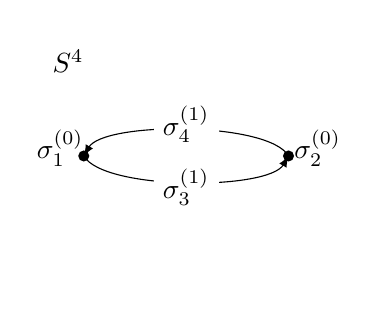
\begin{tikzpicture}
				  \coordinate (1) at (-1.3cm,0cm);
				  \coordinate (2) at (1.3cm,0cm);
				  \draw[-latex, looseness=0.5] (1) to[out=-60, in=240] (2);
				  \draw[latex-, looseness=0.5] (1) to[out=60, in=-240] (2);
				  \draw[color=white, looseness=1.6] (1) to[out=-90, in=270] (2);
				  \draw[color=white, looseness=1.6] (1) to[out=90, in=-270] (2);
				  \fill (canvas cs:x=-1.3cm,y=0cm) circle (2pt);
				  \fill (canvas cs:x=1.3cm,y=0cm) circle (2pt);
				  \node at (-1.6,0.1) {$\sigma_1^{(0)}$};
				  \node at (1.67,0.1) {$\sigma_2^{(0)}$};
				  \node[fill=white] at (0,-0.4) {$\sigma_3^{(1)}$};
				  \node[fill=white] at (0,0.4) {$\sigma_4^{(1)}$};
				  \node at (-1.5,1.2) {$S^4$};
				\end{tikzpicture}
	    }%
	    \hfill
	    \subfloat{
		        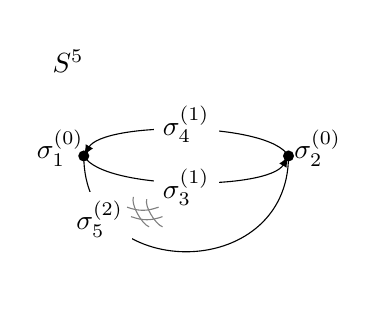
\begin{tikzpicture}
				  \coordinate (1) at (-1.3cm,0cm);
				  \coordinate (2) at (1.3cm,0cm);
				  \draw[-latex, looseness=0.5] (1) to[out=-60, in=240] (2);
				  \draw[latex-, looseness=0.5] (1) to[out=60, in=-240] (2);
				  \draw[looseness=1.6] (1) to[out=-90, in=270] (2);
				  \draw[color=white, looseness=1.6] (1) to[out=90, in=-270] (2);
				  \fill (canvas cs:x=-1.3cm,y=0cm) circle (2pt);
				  \fill (canvas cs:x=1.3cm,y=0cm) circle (2pt);
				  \node at (-1.6,0.1) {$\sigma_1^{(0)}$};
				  \node at (1.67,0.1) {$\sigma_2^{(0)}$};
				  \node[fill=white] at (0,-0.4) {$\sigma_3^{(1)}$};
				  \node[fill=white] at (0,0.4) {$\sigma_4^{(1)}$};
				  \node[fill=white] at (-1.1,-0.8) {$\sigma_5^{(2)}$};
				  \coordinate (a) at (-0.67cm,-0.52cm);
				  \coordinate (b) at (-0.47cm,-0.9cm);
				  \coordinate (c) at (-0.75cm,-0.65cm);
				  \coordinate (d) at (-0.35cm,-0.65cm);
				  \coordinate (c') at (-0.7cm,-0.77cm);
				  \coordinate (d') at (-0.3cm,-0.77cm);
				  \coordinate (a') at (-0.5cm,-0.55cm);
				  \coordinate (b') at (-0.3cm,-0.9cm);
				  \draw[color=gray, looseness=0.6] (a) to[out=250, in=160] (b);
				  \draw[color=gray, looseness=1] (c) to[out=-20, in=200] (d);
				  \draw[color=gray, looseness=1] (c') to[out=-20, in=200] (d');
				  \draw[color=gray, looseness=0.6] (a') to[out=250, in=160] (b');
				  \node at (-1.5,1.2) {$S^5$};
				\end{tikzpicture}
	    }%
	    \hfill
	    \subfloat{
		        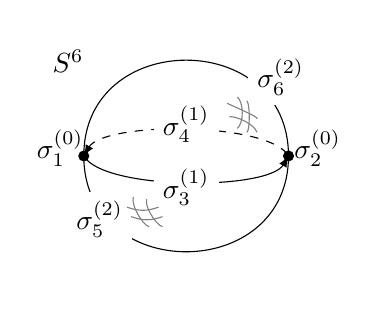
\begin{tikzpicture}
				  \coordinate (1) at (-1.3cm,0cm);
				  \coordinate (2) at (1.3cm,0cm);
				  \draw[-latex, looseness=0.5] (1) to[out=-60, in=240] (2);
				  \draw[latex-, dashed, looseness=0.5] (1) to[out=60, in=-240] (2);
				  \draw[looseness=1.6] (1) to[out=-90, in=270] (2);
				  \draw[looseness=1.6] (1) to[out=90, in=-270] (2);
				  \fill (canvas cs:x=-1.3cm,y=0cm) circle (2pt);
				  \fill (canvas cs:x=1.3cm,y=0cm) circle (2pt);
				  \node at (-1.6,0.1) {$\sigma_1^{(0)}$};
				  \node at (1.67,0.1) {$\sigma_2^{(0)}$};
				  \node[fill=white] at (0,-0.4) {$\sigma_3^{(1)}$};
				  \node[fill=white] at (0,0.4) {$\sigma_4^{(1)}$};
				  \node[fill=white] at (-1.1,-0.8) {$\sigma_5^{(2)}$};
				  \node[fill=white] at (1.2,1) {$\sigma_6^{(2)}$};
				  \coordinate (a) at (-0.67cm,-0.52cm);
				  \coordinate (b) at (-0.47cm,-0.9cm);
				  \coordinate (c) at (-0.75cm,-0.65cm);
				  \coordinate (d) at (-0.35cm,-0.65cm);
				  \coordinate (c') at (-0.7cm,-0.77cm);
				  \coordinate (d') at (-0.3cm,-0.77cm);
				  \coordinate (a') at (-0.5cm,-0.55cm);
				  \coordinate (b') at (-0.3cm,-0.9cm);
				  \draw[color=gray, looseness=0.6] (a) to[out=250, in=160] (b);
				  \draw[color=gray, looseness=1] (c) to[out=-20, in=200] (d);
				  \draw[color=gray, looseness=1] (c') to[out=-20, in=200] (d');
				  \draw[color=gray, looseness=0.6] (a') to[out=250, in=160] (b');
				  \coordinate (e) at (0.52cm,0.67cm);
				  \coordinate (f) at (0.9cm,0.47cm);
				  \coordinate (g) at (0.65cm,0.75cm);
				  \coordinate (h) at (0.65cm,0.35cm);
				  \coordinate (e') at (0.77cm,0.7cm);
				  \coordinate (f') at (0.77cm,0.3cm);
				  \coordinate (g') at (0.55cm,0.5cm);
				  \coordinate (h') at (0.9cm,0.3cm);
				  \draw[color=gray, looseness=0.3] (e) to[out=-30, in=20] (f);
				  \draw[color=gray, looseness=0.7] (g) to[out=-40, in=40] (h);
				  \draw[color=gray, looseness=0.7] (g') to[out=0, in=-250] (h');
				  \draw[color=gray, looseness=0.3] (e') to[out=-30, in=20] (f');
				  \node at (-1.5,1.2) {$S^6$};
				\end{tikzpicture}
	    }%
	\end{figure}

	\begin{itemize}
		\item[$\mathcal{S}^{2}:$] $\emptyset$
		\item[$\subset$] $S^{1} := \{\sigma_{1}^{(0)}\}$
		\item[$\subset$] $S^{2} := \{\sigma_{1}^{(0)}, \sigma_{2}^{(0)}\}$
		\item[$\subset$] $S^{3} := \{\sigma_{1}^{(0)}, \sigma_{2}^{(0)}, \sigma_{3}^{(1)} := (\sigma_{1}^{(0)}, \sigma_{2}^{(0)})\}$
		\item[$\subset$] $S^{4} := \{\sigma_{1}^{(0)}, \sigma_{2}^{(0)}, \sigma_{3}^{(1)}, \sigma_{4}^{(1)} := (\sigma_{2}^{(0)}, \sigma_{1}^{(0)})\}$
		\item[$\subset$] $S^{5} := \{\sigma_{1}^{(0)}, \sigma_{2}^{(0)}, \sigma_{3}^{(1)}, \sigma_{4}^{(1)}, \sigma_{5}^{(2)} := (\sigma_{3}^{(1)}, \sigma_{4}^{(1)})\}$
		\item[$\subset$] $S^{6} := \{\sigma_{1}^{(0)}, \sigma_{2}^{(0)}, \sigma_{3}^{(1)}, \sigma_{4}^{(1)}, \sigma_{5}^{(2)}, \sigma_{6}^{(2)} := (\sigma_{4}^{(1)}, \sigma_{3}^{(1)})\}.$
	\end{itemize}
\end{example}
\vspace{0.2cm}

\section{Persistence Modules}
\label{PersistenceModules}
Persistent homology\index{homology}\index{persistent homology\index{homology}} is derived by applying the homology\index{homology} functor to a filtration\index{filtration} of a topological space. This section will examine the concept of persistent modules\index{modules}, which serve to describe persistent homology\index{homology}\index{persistent homology\index{homology}} from an algebraic perspective. Similarly, as filtrations\index{filtrations} describe the evolution of a simplicial complex under a one-parameter or multi-parameter family, the persistence module describes the evolution of associated vector spaces. In the case of homology\index{homology} vector spaces or modules\index{modules}, the dimension or rank of the associated homomorphisms are the $k$th Betti numbers, which indicates the number of $k$-dimensional holes of a topological space in intuitive terms.

\begin{definition}[Persistence module]{\cite[\S 1.1]{chazal2016structure}}
A real persistence module $\mathcal{V}$ is a collection of vector spaces $\{V_i\}_{i \in I}$ over a partially ordered index set $(I,\leq)$ together with linear maps
\begin{align}
\phi_{r}^{s}: V_r \rightarrow V_s, \quad \forall r,s \in I: r \leq s,
\end{align}
such that $\phi_{r}^{t} = \phi^{t}_{s} \circ \phi_{r}^{s}$ and $\phi_{r}^r = \mathbb{I}_{V_r}$ for all $r \leq s \leq t$.
\end{definition}

We rephrase this definition in categorical language, which makes it easier for us to define the normal form of persistence modules\index{modules}\index{persistence modules\index{modules}}. Persistence modules\index{modules}\index{persistence modules\index{modules}} have a decomposition into interval modules\index{modules}, which cannot be further decomposed. On the other hand, an interval module is a persistence module that is indecomposable. Let $\operatorname{Vect}_\F$ be the category of finite dimensional vector spaces over $\F$. The reals are a partially ordered category $(\R, \leq)$. Consider the real persistence module:

\begin{definition}[Persistence Module]{\cite[\S 1.3]{chazal2016structure}}
A persistence module is a functor $\mathcal{V}: (\R,\leq) \rightarrow \operatorname{Vect}_\F$. It is uniquely defined by a family $\{V_r\}_{r\in\R}$ of finite dimensional vector spaces over $\F$ together with morphisms $\phi_{r}^{s}: V_r \rightarrow V_s, r \leq s$, such that the following diagram commutes:
\begin{equation}
\begin{tikzcd}
V_r \arrow[d, "{\phi_{r}^{t}}" description] \arrow[r, "{\phi_{r}^{s}}" description] & V_s \\
V_t. \arrow[ru, "{\phi_{t}^{s}}" description]                                      &    
\end{tikzcd}
\end{equation}
\end{definition}

\begin{remark}
A morphism of persistence modules\index{modules}\index{persistence modules\index{modules}} is a natural transformation. This can be written as a morphism $f_r: V_r \rightarrow V'_r$, which is compatible with the maps $\phi_{r}^{s}$. This defines the category $\mathrm{Pers}$ of persistence modules\index{modules}\index{persistence modules\index{modules}}.
\end{remark}

The category of persistence modules\index{modules}\index{persistence modules\index{modules}} is abelian. A notable consequence of the aforementioned results is that a part of the constructions for persistence modules\index{modules}\index{persistence modules\index{modules}} remain valid when the category of finite-dimensional vector spaces over a field is replaced by another abelian category. This includes, for instance, (in)finite dimensional vector spaces over other fields. It is also possible to consider persistence modules\index{modules}\index{persistence modules\index{modules}} over cochain complexes in place of vector spaces.

In the following, we will make a number of simplifying assumptions:

\begin{assume}\noindent
\begin{enumerate}
	\item For all $r \in \R\backslash S$, where $S$ is a finite subset, there exists a neighbourhood $U_r$ of $r$ such that the map $\phi_u^{u'}$ is an isomorphism for all $u \leq u'$ in $U_r$.
	\item $V_u = 0$ for $u$ sufficiently small.
	\item For all $t \in \R$ and for all $s \leq t$ with $t-s$ sufficiently small, the mapping $\phi_s^t$ is an isomorphism.
\end{enumerate}
\end{assume}

The assumptions 1, 2 are referred to as finite type conditions. Assumption 1 implies that there is a finite number of 'jumps', while we have that $V_u = V_\infty$ for $u$ large enough. Assumption 3 is called semi-continuity and can be visualised by the following indecomposable interval modules\index{modules}:

\begin{definition}[Interval module]
Let $I$ be an interval of the form $(a,b]$ or $(a,\infty)$ with $-\infty < a < b \leq \infty$. We define an interval module $\mathbb{F}(I)$ over a field $\mathbb{F}$ as follows:
\begin{align}
	\mathbb{F}(I)_t = 
	\begin{cases}
		\mathbb{F}, & \text{if} \; t \in I, \\
		0, & \text{otherwise}.
	\end{cases}
\end{align}
The structure maps $f_{s}^t: \mathbb{F}(I)_s \to \mathbb{F}(I)_t$ for $s \leq t$ are defined as:
\begin{align}
	f_{s}^t = 
	\begin{cases}
		\mathrm{id}_{\mathbb{F}}, & \text{if } s, t \in I, \\
		0, & \text{if } s \notin I \text{ or } t \notin I.
	\end{cases}
\end{align}
\end{definition}

\subsection{Decomposition of Persistence Modules}
The following theorem describes the decomposition of any persistence module:

\begin{theorem}[Decomposition]{\cite[\S 1.5]{chazal2016structure}}
\label{decompositionPersistenceModules}
Every persistence module $\mathcal{V}$ over a field $\mathbb{F}$ is isomorphic to a direct sum of interval modules\index{modules}:
\begin{align}
	\mathcal{V} \cong \bigoplus_{i=0}^{d} \mathbb{F}(I_i)^{m_i},
\end{align}
where $I_i \neq I_j$ for all $i \neq j$, and $m_i$ are multiplicities. This decomposition is unique up to isomorphism and permutation of the summands.
\end{theorem}

\begin{proof}
To establish the existence of such a decomposition, we define a functor from the category $\mathrm{Pers}$ of persistence modules\index{modules}\index{persistence modules\index{modules}} to the category of finitely generated graded modules\index{modules} over the polynomial ring $\mathbb{F}[t]$. For a persistence module $\mathcal{V} = \{V_t, f_{s}^t\}_{s \leq t}$, we map $\mathcal{V}$ to the graded $\mathbb{F}[t]$-module $M = \bigoplus_{t \in \mathbb{R}} V_t$, where the action of $t$ on $M$ is defined by $t \cdot (v_0, v_1, \ldots) := (0, f_{0,1}(v_0), f_{1,2}(v_1), \ldots)$. The conditions ensuring the persistence module structure (finite generation and compatible transition maps) imply that $M$ is finitely generated as an $\mathbb{F}[t]$-module. This functor is an equivalence of categories: the inverse functor takes a graded $\mathbb{F}[t]$-module and interprets the grading as a persistence parameter over $\mathbb{R}$. Since $\mathbb{F}[t]$ is a principal ideal domain (PID), we can apply the structure theorem for finitely generated modules\index{modules} over a PID \cite[\S 2.1]{zomorodian2004computing}, which yields:
\begin{align}
	M = \bigoplus_{t \in \mathbb{R}} V_t \cong \bigoplus_{i=0}^d T^{\alpha_i} \mathbb{F}[t] \oplus \bigoplus_j T^{\gamma_j} \mathbb{F}[t] / (t^{d_j}).
\end{align}
Here, \( T^{\alpha_i} \mathbb{F}[t] \) denotes the graded free module over \( \mathbb{F}[t] \) shifted by \( \alpha_i \), meaning \( (T^{\alpha_i} \mathbb{F}[t])_d = \mathbb{F}[t]_{d - \alpha_i} \). This corresponds to interval modules\index{modules} of the form \( (\alpha_i, \infty) \). Similarly, \( T^{\gamma_j} \mathbb{F}[t] / (t^{d_j}) \) represents a torsion module over \( \mathbb{F}[t] \) that is shifted by \( \gamma_j \), defined by \( (T^{\gamma_j} \mathbb{F}[t] / (t^{d_j}))_d = \mathbb{F}[t]_{d - \gamma_j} / (t^{d_j}) \). This corresponds to interval modules\index{modules} of the form \( (\gamma_j, \gamma_j + d_j] \). 

For uniqueness, consider the endomorphism ring $\text{End}(\mathbb{F}(I))$. We show that $\text{End}(\mathbb{F}(I)) \cong \mathbb{F}$. Any endomorphism $\phi: \mathbb{F}(I) \to \mathbb{F}(I)$ must respect the persistence module structure, meaning $\phi_t: \mathbb{F}(I)_t \to \mathbb{F}(I)_t$ must be a linear map. Since $\mathbb{F}(I)_t = \mathbb{F}$ for $t \in I$ and $0$ otherwise, $\phi_t$ must be multiplication by a scalar $\lambda_t \in \mathbb{F}$. The critical technical reason for this is that $\mathbb{F}(I)_t$ is a simple module (i.e., it has no non-trivial submodules) when $t \in I$. Furthermore, for the endomorphism to be compatible with the structure maps $f_{s}^t$, we must have $\lambda_s = \lambda_t$ for all $s, t \in I$, meaning $\phi$ acts as multiplication by a constant $\lambda \in \mathbb{F}$ uniformly across the entire interval $I$. Hence, $\text{End}(\mathbb{F}(I)) \cong \mathbb{F}$.

Now, suppose we have two decompositions:
\begin{align}
	\bigoplus_i \mathbb{F}(I_i) \cong \mathcal{V} \cong \mathcal{V}' \cong \bigoplus_j \mathbb{F}(J_j).
\end{align}
Consider the composition of morphisms:
\begin{align}
	f_{ij}: &\mathbb{F}(I_i) \hookrightarrow \mathcal{V} \cong \mathcal{V}' \twoheadrightarrow \mathbb{F}(J_j),\\
	g_{ij}: &\mathbb{F}(J_j) \hookrightarrow \mathcal{V}' \cong \mathcal{V} \twoheadrightarrow \mathbb{F}(I_i).
\end{align}
The equation $\sum_{i,j} g_{ij}f_{ij} = 1$ implies that at least one of the compositions $f_{ij}g_{ij} \neq 0$, yielding an isomorphism between $\mathbb{F}(I_i)$ and $\mathbb{F}(J_j)$ for some $i, j$. Since the interval modules\index{modules} are indecomposable and distinct intervals $I_i$ and $J_j$ cannot yield non-trivial morphisms between each other, this forces $I_i = J_j$ and $m_i = m_j$. 

By induction on the number of summands, we conclude that the multiplicities $m_i$ and the intervals $I_i$ in both decompositions must coincide.
\end{proof}

\begin{definition}[Barcode\index{barcode}]
The barcode\index{barcode} associated with a persistence module $\mathcal{V}$ is a collection of tuples consisting of interval modules\index{modules} and their corresponding multiplicities, given by the decomposition in Theorem \ref{decompositionPersistenceModules}:
\begin{align}
	\mathcal{B}(\mathcal{V}) := \{(I_i, m_i)\}_{i=0}^d.
\end{align}
Here, each $I_i$ is an interval, and $m_i$ is the multiplicity of the interval module $\mathbb{F}(I_i)$ in the decomposition of $\mathcal{V}$.
\end{definition}

At this point, we can establish a connection to spectral theory. In particular, for real-valued filtrations\index{filtrations}, the spectrum of a persistence module $\mathcal{V}$ can be represented by specific intervals arising from the decomposition of persistence modules\index{modules}\index{persistence modules\index{modules}}.

\begin{definition}[Spectrum]
A point $t \in \mathbb{R}$ is called a spectral point of a persistence module $\mathcal{V}$ if, for every neighborhood $U_t$ of $t$, there exist $s < r$ in $U_t$ such that the map $f_{s}^t$ is not an isomorphism. The (finite) spectrum of $\mathcal{V}$ is defined as:
\begin{align}
	\text{Spec}(\mathcal{V}) := \{ \text{spectral points} \} \cup \{\infty\}.
\end{align}
\end{definition}

\newpage
\begin{remark}\noindent
\begin{itemize}
    \item For each interval $I = (a,b]$ or $(a,\infty)$, and for any two points $s < r$ within this interval, the corresponding structure map $f_{s}^r$ of the persistence module $\mathcal{V}$ is an isomorphism. A point $t$ becomes a spectral point if, within any neighborhood $U_t$ around $t$, there exists a pair $(s, r)$ such that the map $f_{s}^r$ is not an isomorphism. This identifies a change in the module's behavior, such as the birth of a new feature or the death of an existing one.
    \item The barcode\index{barcode} $\mathcal{B}(\mathcal{V})$ provides a visual and combinatorial representation of the intervals and their multiplicities. Each interval in the barcode\index{barcode} corresponds to a range of points $t$ on the real line where the persistence module maintains consistent behavior. A spectral point indicates a transition between these behaviors, which corresponds to the endpoints of intervals in the barcode\index{barcode}.
    \item The spectrum $\text{Spec}(\mathcal{V})$ summarizes the critical values on the real line where the module's structure changes. This concept is similar to the spectrum in functional analysis, where one considers the set of scalars (like eigenvalues) that describe how a linear operator acts on a vector space.
    \item Since the persistence module $\mathcal{V}$ is finitely generated, the set of intervals in its decomposition is finite. This implies that the set of spectral points, which correspond to transitions between intervals, is also finite. The inclusion of $\infty$ in $\text{Spec}(\mathcal{V})$ represents the asymptotic behavior of $\mathcal{V}$, capturing the intervals of the form $(a, \infty)$.
\end{itemize}
\end{remark}

\subsection{Persistent Homology on Complexes}
\label{PersistentHomologyonComplexes}
In the context of algebraic topology\index{topology}, applying the homology\index{homology} functor $H(-)$
to a finite filtration\index{filtration} of a topological space $\mathcal{X}$ yields a sequence of algebraic structures:
\begin{equation}
	H(\mathcal{X}): \quad H(X^0) \rightarrow H(X^{1}) \to H(X^{2}) \to \cdots
	\to H(X^{d}) \rightarrow H(X),
\end{equation}
where $H(-)$ generally represents either the $k$-th dimensional
homology\index{homology}, denoted by $H_{k}(-;\F)$, or the absolute homology\index{homology}, expressed as $H
_{\bullet}(-;\F)$. Here, this diagram characterizes a sequence of abelian
groups or finite-dimensional vector spaces, connected through linear maps, forming a persistence module. Persistence modules\index{modules}\index{persistence modules\index{modules}} are central to understanding how the features of a space evolve
over time. According to Theorem \ref{decompositionPersistenceModules}, they can be decomposed into interval modules\index{modules}. Each interval module is associated with an
ordered pair of integers $(p,q)$ where $0 \leq p \leq q \leq d$, within a finite
filtration\index{filtration}. These pairs $(p,q)$ signify topological features\index{topological features} that persist over an
index set $I := \{p, \ldots, q\}$, where $\inf\{I\} = p$ and $\sup\{I\} = q$. Conventionally,
these tuples are interpreted as half-open intervals $[a_{p}, a_{q+1})$, with $a_{d+1}
= \infty$ being a customary notation when the sequence extends beyond the largest
indexed space. The decomposition of a persistence module into its constituent interval modules\index{modules} is
represented in a persistence diagram or a barcode\index{barcode}. This barcode\index{barcode} is a multiset of ordered tuples $(p,q)$ or, alternatively, a multiset
of half-open intervals $[a_{p}, a_{q+1})$. This collection is formally expressed
through the forgetful functor $\mathrm{Pers}(-)$, called the persistence diagram:
\begin{align}
    \mathrm{Pers}(H_k(\mathcal{X};\F)) & = \{(p_{1},q_{1}), \ldots, (p_{m},q_{m})\}                    \\
                                           & \cong \{[a_{p_1}, a_{q_1+1}), \ldots, [a_{p_m}, a_{q_m+1})\}.
\end{align}
In practical applications, intervals where $a_{p} = a_{q+1}$ are usually omitted,
as they represent ephemeral topological features\index{topological features}.

\begin{example}{\cite[\S 2.3, Example]{de2011dualities}}
    We consider the topological subspaces $S^{1}$,
    $S^{3}$, $S^{5}$, all of which are contractible. Meanwhile,
    $S^{2}$, $S^{4}$, $S^{6}$ are homeomorphic to the $0$-sphere, $1$-sphere, and $2$-sphere,
    respectively. This structural distinction leads to four distinct intervals in
    the persistence diagram of the absolute homology\index{homology} of a sphere, specifically $\mathcal{S}^{2}$:
    \begin{align}
        \mathrm{Pers}(H_{\bullet}(\mathcal{S}^{2})) & = \{(1,6)_{0}, (2,2)_{0}, (4,4)_{1}, (6,6)_{2} \}             \nonumber\\
                                                    & \cong \{[1,\infty)_{0}, [2,3)_{0}, [4,5)_{1}, [6, \infty)_{2} \}.
    \end{align}
    Here, the subscript $k$ in $(p,q)_{k}$ or $[a_{p}, a_{q+1})_{k}$ denotes a topological
    feature in the $k$-dimensional homology\index{homology}.
\end{example}

\subsection{The Four Standard Persistence Modules}
\label{TheFourStandardPersistenceModules}
\begin{figure}[t!]
	\begin{align*}
		H_{\bullet}(\mathcal{X})             & : \quad H_{\bullet}(X^{0}) \rightarrow H_{\bullet}(X^{1}) \rightarrow \cdots \rightarrow H_{\bullet}(X^{d-1}) \rightarrow H_{\bullet}(X^{d}),             \\
		H^{\bullet}(\mathcal{X})             & : \quad H^{\bullet}(X^{0}) \leftarrow H^{\bullet}(X^{1}) \leftarrow \cdots \leftarrow H^{\bullet}(X^{d-1}) \leftarrow H^{\bullet}(X^{d}),                \\
		H_{\bullet}(X^{\infty}, \mathcal{X}) & : \quad H_{\bullet}(X^{d}) \rightarrow H_{\bullet}(X^{d},X^{0}) \rightarrow H_{\bullet}(X^{d},X^{1}) \rightarrow \cdots \rightarrow H_{\bullet}(X^{d},X^{d-1}), \\
		H^{\bullet}(X^{\infty}, \mathcal{X}) & : \quad H^{\bullet}(X^{d}) \leftarrow H^{\bullet}(X^{d},X^{0}) \leftarrow H^{\bullet}(X^{d},X^{1}) \leftarrow \cdots \leftarrow H^{\bullet}(X^{d}, X^{d-1}).
	\end{align*}
	\caption{The four standard persistence modules are from top to bottom: persistent absolute homology, persistent absolute cohomology, persistent relative homology and persistent relative cohomology. The $(\bullet)$ indicates the direct sum of (co)homology over dimension, in other words the absolute (co)homology. We can also write $H^{\bullet}(X^{d}, \mathcal{X}), H_{\bullet}(X^{d}, \mathcal{X})$ or $H^{\bullet}(X, \mathcal{X}), H_{\bullet}(X, \mathcal{X})$ instead of $H^{\bullet}(X^{\infty}, \mathcal{X}), H_{\bullet}(X^{\infty}, \mathcal{X})$, as the $k$th homology groups for $k > d$ become trivial.}
\end{figure}
The standard module of absolute persistent homology\index{homology}\index{persistent homology\index{homology}}, $H_{\bullet}(\mathcal{X})$, illustrates how the absolute homology\index{homology} groups
$H_{\bullet}(X_{i})$ relate to each other as the index $i$ changes. Similar observations
can be made by considering the absolute cohomology\index{cohomology} groups $H^{\bullet}(X_{i})$,
the relative homology\index{homology} groups $H_{\bullet}(X_{d}, X_{i})$, and the relative cohomology\index{cohomology}
groups $H^{\bullet}(X_{d}, X_{i})$ \cite[\S 2.4]{de2011dualities}. The persistence diagram for absolute cohomology\index{cohomology} is represented as a multiset of integer
pairs $(p,q)$, where $0 \leq p \leq q \leq d$ for a finite filtration\index{filtration}. For relative
homology\index{homology} and cohomology\index{cohomology}, the persistence diagram consists of a multiset of
tuples $(p,q)$ where $0 \leq p \leq q \leq d-1$ for a finite filtration\index{filtration}. In each
case, we interpret $(p,q)$ as a half-open interval $[a_{p}, a_{q+1})$ with the
convention that $a_{0} = -\infty$ and $a_{d+1} = \infty$.

\begin{example}{\cite[\S 2.4, Example]{de2011dualities}}
	For $\mathcal{S}^{2}$ we yield
	\begin{align}
		\mathrm{Pers}(H_{\bullet}(S_{6},\mathcal{S}^{2})) & = \{(0,0)_{0}, (2,2)_{1}, (4,4)_{2}, (0,5)_{2}\}               \\
		                                                  & \cong \{[-\infty, 1)_{0}, [2,3)_{1}, [4,5)_{2}, [-\infty,6)_{3}\}.
	\end{align}
	At index $2$ there is a nontrivial element of $H_{1}(S_{6},S_{2})$ represented
	by any arc connecting the two points of $S_{2}$ --
	the homology\index{homology} class is $[\sigma_{3}] = [\sigma_{4}]$. This class vanishes in $H_{1}(S_{6},S_{3})$, thus we yield the interval $[2,3)$.
\end{example}

\section{Persistent (Co)homology}
\label{Persistent(Co)homology}
Inverse problems primarily involve inferring geometric shapes from measurements like
path integrals. Classical methods such as Fourier transforms provide extensive
information but struggle with nonlinearity and ill-posed conditions, requiring substantial
regularisation. Topology\index{topology}, particularly through persistent homology\index{homology}\index{persistent homology\index{homology}}, offers
alternative methods for deducing topological rather than geometric information. This
approach is especially useful in high-dimensional, discrete sets of points, exemplified
in the finite case by geological sonar to detect subterranean features based on density
variations \cite[\S 1]{de2011dualities}. Persistent homology\index{homology}\index{persistent homology\index{homology}} identifies
topological features\index{topological features} represented as intervals in a barcode\index{barcode} or persistence
diagram, crucial for understanding the presence and persistence of features such
as holes or voids in topological spaces. This method is statistically robust and
can provide both qualitative and quantitative insights into point sets, which we
suspect to lie on some compact topological object \cite{chazal2014persistence,chazal2009proximity}. We follow the results
of de Silva, Morozov, and Vejdemo-Johansson for our explanations \cite[\S 1]{de2011dualities}. In particular, there are at least four naturally arising persistent objects that
can be extracted from a filtration\index{filtration} of any topological space.
They are
\begin{equation*}
	\text{persistent}
	\begin{Bmatrix}
		\text{absolute} \\
		\text{relative}
	\end{Bmatrix}
	\begin{Bmatrix}
		\text{homology\index{homology}}   \\
		\text{cohomology\index{cohomology}}
	\end{Bmatrix}.
\end{equation*}
We address the computation of barcodes for all four types of persistent
objects. We demonstrate that both absolute and relative (co)homologies yield identical
barcodes and that transitions between these states are facilitated by established
duality principles. The duality between homology\index{homology} and cohomology\index{cohomology} is akin to the
duality in vector spaces, whereas a global duality specific to persistent topology\index{topology}
allows for a unique interchange:
\begin{align*}
	\text{Absolute homology\index{homology}}   & \rightleftarrows \text{relative cohomology\index{cohomology}.} \\
	\text{Absolute cohomology\index{cohomology}} & \rightleftarrows \text{relative homology\index{homology}.}
\end{align*}
The main results suggest that a single calculation is sufficient
to compute all four persistent objects due to the commutative nature of the global
duality.

\subsection{Barcode Isomorphisms}
\label{BarcodeIsomorphisms}
We characterise the multisets for persistence modules\index{modules}\index{persistence modules\index{modules}} that are decomposable into
interval modules\index{modules}. The persistence diagram partitions into $\mathrm{Pers}_{0}$,
comprising finite intervals $[a, b)$ as per \cite[\S 2.3]{de2011dualities}, and $\mathrm{Pers}_{\infty}$, consisting of intervals $[a, \infty)$. This leads to the decomposition
$\mathrm{Pers}= \mathrm{Pers}_{0} \cup \mathrm{Pers}_{\infty}$.

In this chapter, we establish that persistent homology\index{homology}\index{persistent homology\index{homology}} and cohomology\index{cohomology} yield the
same intervals, or barcodes, for both absolute and relative (co-)homology\index{homology}
frameworks. This equivalence necessitates invoking the Universal Coefficients Theorem
from algebraic topology\index{topology}, which we will prove beforehand. The universal coefficient
theorem for cohomology\index{cohomology} elegantly ties together the cohomology\index{cohomology} of a space with coefficients
in any abelian group $G$ to the homology\index{homology} of the space with integer coefficients. Specifically, as notation for this proof, $H_{d}(X;\mathbb{Z})$ and
$H^{d}(X;\mathbb{Z})$ denote the $d$-th singular homology\index{homology} and cohomology\index{cohomology} groups
with coefficients in $\mathbb{Z}$, respectively. We further involve
$\operatorname{Hom}(A, G)$, denoting group homomorphisms from an abelian group $A$ to another
abelian group $G$, and $\operatorname{Ext}^{1}(A, G)$ \cite[\S 3.1, p.195]{hatcher2005algebraic}, which measures obstructions
in the splitting of a short exact sequence of abelian groups. Further, we use the
properties of derived functors \cite[\S 2.7]{Weibel1994}.

\begin{theorem}[Universal coefficients for cohomology\index{cohomology}]{\cite[Theorem 3.2]{hatcher2005algebraic}}
\label{UniversalCoefficientsforCohomology}
Let $X$ be a topological space and $G$ an abelian group. For any integer $d \geq 0$, there is a short exact sequence:
\begin{align}
0 \rightarrow &\operatorname{Ext}^{1}(H_{d-1}(X;\mathbb{Z}), G) \rightarrow H^{d}(X; G) \rightarrow \cdots \\
\cdots \rightarrow &\operatorname{Hom}(H_{d}(X;\mathbb{Z}), G) \rightarrow 0,
\end{align}
which splits, though not canonically.
\end{theorem}

\begin{proof}
Let $(\mathcal{C}(X),\partial)$ be the singular chain complex of a topological space $X$ with integer coefficients. The homology\index{homology} groups $H_{d}(X; \mathbb{Z})$ are defined as:
\begin{align}
H_{d}(X; \mathbb{Z}) := \ker(\partial_{d}) / \operatorname{im}(\partial_{d+1}),
\end{align}
where $\partial_{d}$ are the boundary maps in $\mathcal{C}(X)$. The chain group $C_{d}(X)$ consists of formal sums of singular $d$-simplices in $X$ with integer coefficients. The boundary maps $\partial_{d}: C_{d}(X) \rightarrow C_{d-1}(X)$ are defined by
\begin{align}
\partial_{d}(\tilde{\sigma}^{(d)}) = \sum_{i=0}^{d}(-1)^{i} \tilde{\sigma}^{(d)}|_{[v_0, \ldots, \hat{v}_i, \ldots, v_d]},
\end{align}
where $\tilde{\sigma}^{(d)}: \tilde{\sigma}^{d} \rightarrow X$ is a singular simplex, and $\tilde{\sigma}|_{[v_0, \ldots, \hat{v}_i, \ldots, v_d]}$ denotes the restriction of $\tilde{\sigma}$ to the $i$-th face of the simplex, omitting the $i$-th vertex. The functor $\operatorname{Hom}(-, G)$ applied to $C_{d}(X)$ yields a group $\operatorname{Hom}(C_{d}(X), G)$, and the coboundary $\delta^{d}$ for the cochain complex $\operatorname{Hom}(\mathcal{C}^\dagger(X), G)$ is $\delta^{d}(f) = f \circ \partial_{d+1}$ for $f \in \operatorname{Hom}(C_{d+1}(X), G)$. This leads to the cohomology\index{cohomology groups} groups $H^{d}(X; G) := \ker(\delta^{d}) / \operatorname{im}(\delta^{d-1})$. We consider the projective resolution of $\mathcal{C}^\dagger(X)$ to effectively apply the $\operatorname{Ext}^1$-functor. For an abelian group $A$, $\operatorname{Ext}^{1}(A, G) = R^{1} \operatorname{Hom}(A, G)$, where $R^{1}$ denotes the first right derived functor of $\operatorname{Hom}$ \cite[Vista 3.4.6, \S 3.5]{Weibel1994}. To show this equality, we begin by taking a projective resolution of $A$ \cite[Definition 2.2.4]{Weibel1994}: $\cdots \to P_{2} \to P_{1} \to P_{0} \to A \to 0$, where each $P_{i}$ is a projective abelian group. Then we can apply the functor $\operatorname{Hom}(-, G)$ to the projective resolution:
\begin{align}
0 \to \operatorname{Hom}(P_{0}, G) \to \operatorname{Hom}(P_{1}, G) \to \operatorname{Hom}(P_{2}, G) \to \cdots.
\end{align}
This sequence is exact on the left because $\operatorname{Hom}(-, G)$ is left exact and each $P_{i}$ is projective. The first right derived functor $R^{1}\operatorname{Hom}(A, G)$ is defined as the cohomology\index{cohomology} of this sequence at $P_{1}$:
\begin{align}
R^{1} \operatorname{Hom}(A, G) = \frac{\ker(\operatorname{Hom}(P_{1}, G) \to \operatorname{Hom}(P_{2}, G))}{\operatorname{im}(\operatorname{Hom}(P_{0}, G) \to \operatorname{Hom}(P_{1}, G))}.
\end{align}
The group $\operatorname{Ext}^{1}(A, G)$ classifies extensions of $A$ by $G$, equivalent to the kernel / image calculation in the cohomology\index{cohomology} of the $\operatorname{Hom}$-sequence $R^{1} \operatorname{Hom}(A, G)$. Given $H_{d}(X; \mathbb{Z})$, consider the short exact sequence obtained from the projective resolution of $\mathbb{Z}$: $0 \rightarrow \mathbb{Z} \rightarrow F \rightarrow H_{d}(X; \mathbb{Z}) \rightarrow 0$, where $F$ is free. Applying $\operatorname{Hom}(-, G)$ gives
\begin{align}
0 \rightarrow &\operatorname{Hom}(H_{d}(X; \mathbb{Z}), G) \rightarrow \operatorname{Hom}(F, G) \rightarrow \cdots \nonumber\\
\cdots \rightarrow &\operatorname{Hom}(\mathbb{Z}, G) \rightarrow \operatorname{Ext}^{1}(H_{d}(X; \mathbb{Z}), G) \rightarrow 0.
\end{align}
We apply $\operatorname{Ext}^{1}$, which gives rise to the long exact sequence of $\operatorname{Ext}^1$-groups:
\begin{align}
0 \rightarrow &\operatorname{Hom}(H_{d}(X; \mathbb{Z}), G) \rightarrow H^{d}(X; G) \rightarrow \cdots \nonumber\\
\cdots \rightarrow &\operatorname{Ext}^{1}(H_{d-1}(X; \mathbb{Z}), G) \rightarrow 0.
\end{align}
Finally, we verify exactness and splitting. The term $\operatorname{Ext}^{1}(H_{d-1}(X; \mathbb{Z}), G)$ measures the non-trivial extensions of $G$ by $H_{d-1}(X; \mathbb{Z})$, which corresponds to the obstructions to lifting $H_{d-1}(X; \mathbb{Z})$ linearly over $G$. The term $\operatorname{Hom}(H_{d}(X; \mathbb{Z}), G)$ represents the group homomorphisms from $H_{d}(X; \mathbb{Z})$ to $G$, which naturally includes in $H^{d}(X; G)$. The sequence is exact at each stage by the properties of derived functors and their application to the singular chain complex \cite[Horseshoe Lemma 2.2.8]{Weibel1994}. The sequence ends with $0$ because $\operatorname{Ext}^{1}$ of a projective (or free) module vanishes, and $\mathbb{Z}$ is free. The sequence splits because the functor $\operatorname{Hom}(-, G)$ preserves products and coproducts. However, the way it splits is not canonical and depends on the choice of a splitting homomorphism, which is not unique.

In the generalization of the Universal Coefficient Theorem \ref{UniversalCoefficientsforCohomology} to the case of modules\index{modules} over a PID, the $\operatorname{Ext}^{1}$ terms vanish since $\F$ is a field, thus we obtain $H^{d}(X;\F) \cong \operatorname{Hom}(H_{d}(X;\F),\F)$ \cite[\S 3.3.1, p.198]{hatcher2005algebraic}.
\end{proof}

\begin{theorem}{\cite[Proposition 2.3]{de2011dualities}}
For all integers $d \geq 0$, it holds that:
\begin{align}
\mathrm{Pers}(H_{d}(\mathcal{X};\F)) &= \mathrm{Pers}(H^{d}(\mathcal{X};\F)), \\
\mathrm{Pers}(H_{d}((X^{\infty}, \mathcal{X});\F)) &= \mathrm{Pers}(H^{d}((X^{\infty}, \mathcal{X});\F)).
\end{align}
\end{theorem}

\begin{proof}
When considering coefficients in a field $\F$ rather than in a ring, the Universal Coefficient Theorem \ref{UniversalCoefficientsforCohomology} assures us of a natural isomorphism between the $d$-th cohomology\index{cohomology} group and the homomorphisms from the $d$-th homology\index{homology} group to the base field: $H^{d}(X; \F) \cong \operatorname{Hom}(H_{d}(X; \F), \F)$. Therefore, the associated maps
\begin{equation}
H_{d}(X^{i}; \F) \rightarrow H_{d}(X^{j}; \F) \quad \text{and} \quad H^{d}(X^{i}; \F) \leftarrow H^{d}(X^{j}; \F)
\end{equation}
are adjoint and hence possess the same rank. Since the persistence intervals over a field are uniquely determined by the dimension and rank of the homology\index{homology} vector spaces, it follows that this holds for both homology\index{homology} and cohomology\index{cohomology}. Consequently, they share the same barcode\index{barcode}.
\end{proof}

Consider a finite filtration\index{filtration} $X^{0} \subset X^{1} \subset X^{2} \subset \cdots \subset X^d \subseteq X^{\infty}$ of a topological space $X$. The homology\index{homology} groups $H_{k}(X^{d})$ for some fixed dimension $k$ serve as the initial terms for the relative homology\index{homology} groups $H_{k}(X^{\infty}, X)$. Since $H_{k}(X)$ is consistent with $H_{k}(X^{d})$ as $d$ approaches infinity, these sequences can be unified into a single sequence: $H_{k}(X) \to H_{k}(X^{\infty}, X)$. For this concatenated sequence, the indices are 
\begin{align}
\{0, 1, 2, \ldots, d = 0^{\flat}, 1^{\flat}, 2^{\flat}, \ldots, (d-1)^{\flat}\},
\end{align}
using the $\flat$ symbol to indicate relative homology\index{homology} part of the sequence. This structure allows us to discuss the persistence diagram associated with this homological configuration. The persistence intervals in this diagram can generally be categorized into three types:
\begin{enumerate}
	\item $(p, q)$ where $0 \leq p \leq q < d$, denoted as $[p, q+1)$ or $[a_{p}, a_{q+1})$.
	\item $(p^{\flat}, q^{\flat})$ where $0 < p \leq q \leq d-1$, denoted as $[p^{\flat}, q^{\flat}+1)$ or $[a_{p^\flat}, a_{q^\flat+1})$.
	\item $(p, q^{\flat})$ where $0 \leq p \leq d, 0 \leq q \leq d-1$, denoted as $[p, q^{\flat}+1)$ or $[a_{p}, a_{q^\flat+1})$.
\end{enumerate}

\begin{corollary}{\cite[Proposition 2.5]{de2011dualities}}
The barcode\index{barcode} $\mathrm{Pers}(H_{k}(\mathcal{X}) \rightarrow H_{k}(X^{\infty}, \mathcal{X}))$ comprises the following collections of intervals, which match the previously discussed types of intervals bijectively:
\begin{enumerate}
    \item An interval $[a, b)$ for every interval $[a, b)$ in $\mathrm{Pers}_{0}(H_{k}(\mathcal{X}))$.
    \item An interval $[a^{\flat}, b^{\flat})$ for every interval $[a, b)$ in $\mathrm{Pers}_{0}(H_{k-1}(\mathcal{X}))$.
    \item An interval $[a, a^{\flat})$ for every interval $[a, \infty)$ in $\mathrm{Pers}_{\infty}(H_{k}(\mathcal{X}))$.
\end{enumerate}
\end{corollary}

\begin{proof}
	We begin by analyzing the first two types of intervals in the persistence diagram
	$\mathrm{Pers}(H_{k}(X) \to H_{k}(X^{\infty}, X))$. These intervals either do
	not intersect the intermediate term $H_{k}(X_{d})$ or terminate before it. Consequently,
	they correspond precisely to the finite intervals in $\mathrm{Pers}(H_{k}(X))$
	and $\mathrm{Pers}(H_{k}(X^{\infty}, X))$, clarifying the first two cases. The
	correspondence $\mathrm{Pers}_{0}(H_{k}(X^{\infty}, X)) = \mathrm{Pers}_{0}(H_{k-1}(X))$
	helps in mapping these relationships.

	The third case requires examining intervals of the form $[a, b^{\flat})$ and
	proving that they are invariably of the form $[a, a^{\flat})$, which means that
	the paired intervals $[a,\infty)$ and $[-\infty,a)$ in $\mathrm{Pers}_{\infty}(
	H_{k}(\X))$ and $\mathrm{Pers}_{\infty}(H_{k}(X^{\infty}, \X))$ are restrictions
	of a single interval $[a,a^{\flat})$ in the concatenated sequence \cite[Proof of Proposition 2.5]{de2011dualities}.
	To establish this, we compare the ascending filtration\index{filtration} defined by the images of
	$H_{k}(X^{i})$ in $H_{k}(X^{d})$ for $i = 0, 1, 2, \ldots, d-1$ (denoted as
	$\operatorname{im}(H_{k}(X^{i}) \to H_{k}(X^{d}))$) with the descending filtration\index{filtration} defined
	by the kernels of $H_{k}(X^{d})$ in $H_{k}(X^{\infty}, X)$ for $i = 0, 1, 2, \ldots
	, d-1$ (denoted as $\ker(H_{k}(X^{d}) \to H_{k}(X^{d}, X^{i}))$). This
	examination revolves around the fundamental properties of the homology\index{homology} groups
	in a filtration\index{filtration} setting. For each index $i$, the image and kernel correspond to the same subspace of $H_{k}
	(X^{d})$. This equivalence is guaranteed by the homology\index{homology} long exact sequence
	associated with the pair $(X^{d}, X^{i})$, which links the relative and absolute
	homology\index{homology} groups. Specifically, the exact sequence implies that any cycle in $\operatorname{im}
	(H_{k}(X^{i}) \to H_{k}(X^{d}))$ that becomes a boundary in $H_{k}(X^{d}, X^{i}
	)$ must vanish, thus equating the image and kernel. As a result, both
	filtrations\index{filtrations} align perfectly, establishing that the third type of interval indeed
	maps to self-closing intervals of the form $[a, a^{\flat})$.
\end{proof}

\subsection{Persistent Chain Complexes}
Alternatively, following \cite[\S 2.6]{de2011dualities}, the standard persistence module
can be described via a filtered cell complex $\mathcal{X}:= \bigcup_{i=0}^{d}\bigcup_{a \in I_d} \sigma_a^{(\natural)}$, adding cells for each filtration step, so that the persistence module is the sequence
\[
	\mathcal{C}: \quad C^{0} \to C^{1} \to C^{2} \to \cdots \to C^{d},
\]
for a finite filtration\index{filtration}, where each $C^{i} := \langle \{\sigma^{(\natural)}_a\}_{a \in I_0}, \{\sigma^{(\natural)}_a\}_{a \in I_1}, \ldots, \{\sigma^{(\natural)}_a\}_{a \in I_i}
\rangle$ is a vector space (or an abelian group) over a field $\F$,
generated by the elements $\sigma^{(\natural)}_a$ for $a \in I_0, I_1, \ldots, I_i$. The boundary operator
is defined by $\partial_{(\natural)} \sigma^{(\natural)}_{j} = \sum_{i<j}\lambda_{ij}\sigma^{(\natural-1)}_{i}$ for $\lambda
_{ij}\in \F$ for all $i, j \in \{0, 1, \ldots, d\}$. Then $\mathcal{C}(X) = \{C_{i},\partial_{i}\}_{i=0}^{d}$ is the chain complex of $X$, and $\mathcal{C}(\mathcal{X})$ represents the persistent version for $\mathcal{X}$. This leads to the definition
of the persistent absolute homology\index{homology} of $\mathcal{X}$ as
\[
	H_{\bullet}(\mathcal{X}) = H(\mathcal{V}, \partial): \quad \frac{\ker(\partial_{1})}{\text{im}(\partial_{1})}
	\to \frac{\ker(\partial_{2})}{\text{im}(\partial_{2})}\to \cdots \to \frac{\ker(\partial_{d})}{\text{im}(\partial_{d})}
	.
\]

For the persistent absolute cohomology\index{cohomology} $H^{\bullet}(\mathcal{X})$, we define
\[
	\mathcal{V}^{\flat}: \quad V^{\flat}_{1} \leftarrow V^{\flat}_{2} \leftarrow \cdots
	\leftarrow V^{\flat}_{d},
\]
where $V_{i}^{\flat} = \text{Hom}(V_{i}, \F) = \langle \{\sigma^{(\natural)\flat}_a\}_{a \in I_1}, \{\sigma^{(\natural)\flat}_a\}_{a \in I_1}, \ldots, \{\sigma^{(\natural)\flat}_a\}_{a \in I_1} \rangle$, with the elements
$\{\sigma^{(\natural)\flat}_a\}_{a\in I_j}$ as the dual basis of $\{\sigma^{(\natural)}_a\}_{a \in I_j}$. The coboundary $\delta
= \partial^{\flat}$ is defined as the adjoint of $\partial$. Then
$V^{\flat}(\mathcal{X}) = (\mathcal{V}^{\flat}, \delta)$ and
$H^{\bullet}(\mathcal{X}) = H(\mathcal{V}^{\flat}, \delta) = \ker(\delta) / \text{im}
(\delta)$. This is a persistence module, with morphisms in the
reverse direction.

\begin{example}
	For $\mathcal{S}^{2}$, the boundary operator is given by
	\begin{align}
		\label{matrix}
		\partial_0\sigma^{(0)}_{1} & = \partial_0\sigma^{(0)}_{2} = 0, \nonumber\\
		\partial_1\sigma_{3}^{(1)} & = \partial_1\sigma_{4}^{(1)} = \sigma_{1}^{(0)}-\sigma_{2}^{(0)}, \nonumber\\
		\partial_2\sigma_{5}^{2} & = \partial_2\sigma_{6}^{(2)} = \sigma_{3}^{(1)} - \sigma_{4}^{(1)}.
	\end{align}
	Similarly, the coboundary operator is given by
	\begin{align}
		\label{transposed}
		\delta^0\sigma_{1}^{(0)\flat} = -\delta^0\sigma_{2}^{(0)\flat} & = \sigma_{3}^{(1)\flat} + \sigma_{4}^{(1)\flat}, \nonumber\\
		\delta^1\sigma_{3}^{(1)\flat} = -\delta^1\sigma_{4}^{(1)\flat} & = \sigma_{5}^{(2)\flat} + \sigma_{6}^{(2)\flat}, \nonumber\\
		\delta^2\sigma_{5}^{(2)\flat} = \delta^2\sigma_{6}^{(2)\flat}  & = 0.
	\end{align}
	The data in Eq. \ref{matrix} and in Eq. \ref{transposed} can be summarized in a matrix and its transposed, respectively. The relative homology\index{homology} and cohomology\index{cohomology} persistence modules\index{modules}\index{persistence modules\index{modules}} are then defined as the homology\index{homology} of the persistence modules\index{modules}\index{persistence modules\index{modules}} \cite[\S 2.6, Example]{de2011dualities}:
	\begin{align}
		(V_{d}/\mathcal{V}):         & \quad V_{d} \rightarrow (V_{d}/V_{1}) \rightarrow (V_{d}/V_{2}) \rightarrow \cdots \rightarrow (V_{d}/V_{d-1}),                             \\
		(V_{d}/\mathcal{V})^{\flat}: & \quad V_{d}^{\flat} \leftarrow (V_{d}/V_{1})^{\flat} \leftarrow (V_{d}/V_{2})^{\flat} \leftarrow \cdots \leftarrow (V_{d}/V_{d-1})^{\flat}.
	\end{align}
	We note that the mappings $\rightarrow$ from $\mathcal{V}$ and the mappings $\leftarrow$
	from $(V_{d}/\mathcal{V})^{\flat}$ are injective, while the mappings
	$\leftarrow$ from $\mathcal{V}^{\flat}$ and the mappings $\rightarrow$ from
	$(V_{d}/\mathcal{V})$ are surjective. Thus, absolute and relative cohomology\index{cohomology}
	are structurally similar but qualitatively different from absolute homology\index{homology}
	and relative homology\index{homology}.
\end{example}

\begin{figure}
\centering
\begin{tikzcd}
                                  & \vdots \arrow[d, "\partial_{k+2}"]                                   & \vdots \arrow[d, "\partial_{k+2}"]                               & \vdots \arrow[d, "\partial_{k+2}"]                                            & \vdots \arrow[d, "\partial_{k+2}"]                                   &        \\
\cdots \arrow[r, "f^{i-2}_{k+1}"] & V_{k+1}^{i-1} \arrow[r, "f^{i-1}_{k+1}"] \arrow[d, "\partial_{k+1}"] & V_{k+1}^{i} \arrow[r, "f^{i}_{k+1}"] \arrow[d, "\partial_{k+1}"] & V_{k+1}^{i+1} \arrow[r, "f^{i+1}_{k+1}", no head] \arrow[d, "\partial_{k+1}"] & V_{k+1}^{i+2} \arrow[d, "\partial_{k+1}"] \arrow[r, "f^{i+2}_{k+1}"] & \cdots \\
\cdots \arrow[r, "f^{i-2}_{k}"]   & V_{k}^{i-1} \arrow[d, "\partial_{k}"] \arrow[r, "f^{i-1}_{k}"]       & V_{k}^{i} \arrow[d, "\partial_{k}"] \arrow[r, "f^{i}_{k}"]       & V_{k}^{i+1} \arrow[d, "\partial_{k}"] \arrow[r, "f^{i+1}_{k}"]                & V_{k}^{i+2} \arrow[d, "\partial_{k}"] \arrow[r, "f^{i+2}_{k}"]       & \cdots \\
\cdots \arrow[r, "f^{i-2}_{k-1}"] & V_{k-1}^{i-1} \arrow[d, "\partial_{k-1}"] \arrow[r, "f^{i-1}_{k-1}"] & V_{k-1}^{i} \arrow[d, "\partial_{k-1}"] \arrow[r, "f^{i}_{k-1}"] & V_{k-1}^{i+1} \arrow[d, "\partial_{k-1}"] \arrow[r, "f^{i+1}_{k-1}"]          & V_{k-1}^{i+2} \arrow[d, "\partial_{k-1}"] \arrow[r, "f^{i+2}_{k-1}"] & \cdots \\
                                  & \vdots                                                               & \vdots                                                           & \vdots                                                                        & \vdots                                                               &       
\end{tikzcd}
\caption[A persistence complex]{A persistent chain complex, where moving to the right increases the filtration\index{filtration} index, while moving downwards decreases the dimension. The maps $f_{i,k}^{i+1}$ correspond to the structure map $f_{i}^{i+1}$ in filtration step $k$. The boundary operator is defined for the chain complex, restricting it for each element to the respective chain group.}
\end{figure}

\begin{theorem}[Partition of persistence modules]
	{\cite[Theorem 2.6]{de2011dualities}} \label{persistencepartition} Let $\mathcal{V}$ be given and $\partial$ as above, then there
	exists a partition $\{1,2, \ldots, d\} = B^{\Join} \sqcup B \sqcup D$ with a bijective pairing $B \leftrightarrow D$, such that $b$ is paired with $d$ if and only if $[b,d) \in \operatorname{Pairs}(\mathcal{V}, \partial)$. Furthermore, there is a basis
	$\hat{\sigma}^{(\natural)}_{1}, \hat{\sigma}^{(\natural)}_{2}, \ldots, \hat{\sigma}^{(\natural)}_{d}$ of $V_{d}$ such
	that
	\begin{itemize}
		\item $V_{i} = \langle \hat{\sigma}^{(\natural)}_{1}, \ldots, \hat{\sigma}^{(\natural)}_{i} \rangle$ for
			each $i$.
		\item $\partial_{(\natural)}\hat{\sigma}^{(\natural)}_{b} = 0$ for all $b \in B^{\Join}$.
		\item $\partial_{(\natural)}\hat{\sigma}^{(\natural)}_{d} = \hat{\sigma}^{(\natural)}_{b}$, and thus
			$\partial_{(\natural)}\hat{\sigma}^{(\natural)}_{b} = 0$, for all $[b,d) \in \operatorname{Pairs}$.
	\end{itemize}
	It follows that the persistence diagram
	$\operatorname{Pers}(H(\mathcal{V},\partial))$ consists of $[a_{b}, \infty)$ for
	$b \in B^{\Join}$ together with intervals $[a_{b},a_{d})$ for
	$[b,d) \in \operatorname{Pairs}$.
\end{theorem}

\begin{proof}
	Let $\mathcal{V}= \{V_{i}\}_{i \in I}$ be a filtered chain complex associated with
	a topological space, structured over a field $\F$ for any finite index
	set $I$. The filtration\index{filtration} indices ${1, 2, \ldots, d}$, where $d = \vert I \vert$,
	classify the stages at which elements are born or die in homology\index{homology}. The
	partition of $\{1, 2, \ldots, d\}$ into $B^{\Join} \sqcup B \sqcup D$ is then constructed such that $B^{\Join}$ contains indices corresponding to elements that persist indefinitely, i.e., those for which $\partial_{(\natural)}\sigma^{(\natural)}_{i} = 0$ and $\sigma^{(\natural)}_{i}$ does not become a boundary at any higher index. $B$ and $D$ are paired bijectively, where each $b \in B$ (births) corresponds uniquely to an $d \in D$ (deaths), signifying the termination of the homological feature introduced at $d$. This pairing is determined through the matrix reduction of $\partial$, ensuring that every cycle born at stage $b$ becomes a boundary at stage $d$. We then construct a basis ${\hat{\sigma}^{(\natural)}_i}$ such that for each $i$, $\hat{\sigma}^{(\natural)}
	_{i}$ is a generator of $C_{i}$. Specifically, if $i \in B^{\Join}$, then
	$\partial_{(\natural)}\hat{\sigma}^{(\natural)}_{i} = 0$, indicating these elements are cycles that persist
	indefinitely. For pairs $[b, d) \in \operatorname{Pairs}(\mathcal{V}, \partial)$
	with $b \in B$ and $d \in D$, set $\partial_{(\natural)}\hat{\sigma}^{(\natural)}_{d} = \hat{\sigma}^{(\natural)}_{b}$
	and $\partial_{(\natural)}\hat{\sigma}_{b} = 0$, reflecting the fact that the cycle
	$\hat{\sigma}^{(\natural)}_{b}$ born at $b$ becomes a boundary at $d$ and thus ceases to
	contribute to homology\index{homology} past $d$. Hence, the persistence diagram $\operatorname{Pers}(H(\mathcal{V}, \partial))$ contains
	intervals $[a_{b}, \infty)$ for each $b \in B^{\Join}$, indicating persistent
	homological features and intervals $[a_{b}, a_{d})$ for each
	$[b, d) \in \operatorname{Pairs}$, describing features with finite lifespans,
	starting as a cycle at $b$ and terminating as a boundary at $d$.
\end{proof}

\begin{remark}
In Theorem \ref{persistencepartition} the index sets can be reexpressed in the original language of positive and negative simplices proposed by Edelsbrunner et al. \cite[p.8]{de2011dualities}, where a $(\natural)$-simplex is called positive if it belongs to a $(\natural)$-cycle and negative if it doesn't, respectively \cite[\S 2, p.516]{Edelsbrunner2000}:
\begin{itemize}
	\item $B$ identifies the positive simplices that remain unpaired,
	\item $B^{\Join}$ identifies the positive simplices that do become paired,
	\item $D$ identifies the negative simplices.
\end{itemize}
The vectors $\hat{\sigma}^{(\natural)}_{b}$ and $\hat{\sigma}^{(\natural)}_{d}$ are cycles characterized by
their leading terms $\sigma^{(\natural)}_{b}$ and $\sigma^{(\natural)}_{d}$ respectively, while the vector
$\hat{\sigma}^{(\natural)}_{d}$ is a chain with leading term $\sigma^{(\natural)}_{d}$. This chain 'kills'
the homology\index{homology} class of its paired cycle $\hat{\sigma}^{(\natural)}_{b}$ through the boundary relation
$\partial_{(\natural)} \hat{\sigma}^{(\natural)}_{d} = \hat{\sigma}^{(\natural)}_{b}$.
\end{remark}

\begin{theorem}{\cite[Proposition 2.4]{de2011dualities}}
	For all integers $d \geq 0$, it holds that:
	\begin{align*}
		\mathrm{Pers}_0(H_{d}(\mathcal{X})) \cong \mathrm{Pers}_0(H_{d+1}(X_\infty, \mathcal{X})), \nonumber\\
		\mathrm{Pers}_\infty(H_{d}(X_{\infty}, \mathcal{X})) \cong \mathrm{Pers}_\infty(H_{d}(X_{\infty}, \mathcal{X})).
	\end{align*}
\end{theorem}

\begin{proof}{\textit{\cite[Proof of Proposition 2.4]{de2011dualities}}}
The decomposition $\{1,2,\ldots,d\} = B^\Join \sqcup B \sqcup D$ and the new basis $\hat{\sigma}^{(\natural)}_1, \hat{\sigma}^{(\natural)}_2, \ldots, \hat{\sigma}^{(\natural)}_d$ allow us to write the persistent chain complex $\mathcal{V}$ as a direct sum of persistent chain complexes, such that
\begin{align}
	\mathcal{V} &= \bigoplus_{b^\Join \in B^\Join} \mathcal{V}_{b^\Join} \oplus \bigoplus_{[b,d) \in \operatorname{Pairs}} \mathcal{V}_{bd} \nonumber\\
	&= \bigoplus_{b^\Join \in B^\Join} \langle \hat{\sigma}_{b^\Join} \rangle \oplus \bigoplus_{[b,d) \in \operatorname{Pairs}} \langle \hat{\sigma}_{b}, \hat{\sigma}_{d} \rangle.
\end{align}
The boundary operator is compatible with this decomposition, where $\partial$ for each summand is defined as the corresponding boundary operator of the chain complex. Therefore, we can compute the homology $H((V_d/\mathcal{V}),\partial)$ separately for each summand. For summands of the form $\mathcal{V}_{b^\Join}$, the persistence modules are constant over two phases, with indices in $\{0,\ldots,b^\Join - 1\}$ and $\{b^\Join, \ldots, d-1\}$. Thus,
\begin{align}
	((V_{b^{\Join}})_d/\mathcal{V}_{b^\Join})&: \quad \langle \hat{\sigma}^{(\natural)}_{b^\Join}\rangle \rightarrow 0,\nonumber\\
	\ker(\partial)&: \quad \langle \hat{\sigma}^{(\natural)}_{b^\Join}\rangle \rightarrow 0,\nonumber\\
	\operatorname{im}(\partial)&: \quad 0 \rightarrow 0,\nonumber\\
	H := \ker(\partial) / \operatorname(im)(\partial)&: \quad \langle \hat{\sigma}^{(\natural)}_{b^\Join}\rangle \rightarrow 0.
\end{align}
It follows that $H((V_{b^\Join})_d/\mathcal{V}_{b^\Join})$ contributes an interval of the form $[-\infty, a_{b^\Join})$, generated by the equivalence class of $[\hat{\sigma}^{(\natural)}_{b^\Join}]$, and thus has the same homological dimension as $[a_{b^{\Join}}, \infty) \in \operatorname{Pers}(H(\mathcal{V}))$. For summands of the type $\mathcal{V}_{bd}$, the persistence modules can be divided into constants over three phases, with indices in the ranges $\{0,\ldots,b-1\},$ $\{b,\ldots,d-1\}$, and $\{d,\ldots, n-1\}$, or explicitly:
\begin{align}
((V_{bd})_n/\mathcal{V}_{bd}) &: \quad \langle \hat{\sigma}^{(\natural)}_b, \hat{\sigma}^{(\natural)}_d \rangle \rightarrow \langle \hat{\sigma}^{(\natural)}_d \rangle \rightarrow 0,\nonumber\\
\ker(\partial) &: \quad \langle \hat{\sigma}^{(\natural)}_b \rangle \rightarrow \langle \hat{\sigma}^{(\natural)}_d \rangle \rightarrow 0, \nonumber\\
\operatorname{im}(\partial) &: \quad \langle \hat{\sigma}^{(\natural)}_b \rangle \rightarrow 0 \rightarrow 0,\nonumber\\
H := \ker{\partial} / \operatorname{im}(\partial) &: \quad 0 \rightarrow \langle \hat{\sigma}^{(\natural)}_b \rangle \rightarrow 0.
\end{align}
It follows that $H((V_{bd})_n/\mathcal{V}_{bd})$ contributes a single interval of the form $[a_b,a_d)$, generated by the equivalence class $[\hat{\sigma}^{(\natural)}_b]$, and thus has one dimension more than $[a_b,a_d) \in \operatorname{Pers}(H(\mathcal{V}))$, which is generated by $[\hat{\sigma}^{(\natural)}_d]$.
\end{proof}

\begin{remark}
	In this case, we get an isomorphism of multisets. This is due to the identification
	of the intervals $[a,\infty) \leftrightarrow [-\infty, a)$ for $\mathrm{Pers}_{\infty}$.
	Thus, persistent homology\index{homology}\index{persistent homology\index{homology}} and relative homology\index{homology} barcodes carry the same information,
	with a dimension shift for the finite intervals \cite[Proposition 2.4]{de2011dualities}.
\end{remark}

In this closing argument, we will prove the four statements in Morozov's paper that were left open for the reader \cite[\S 2.8]{de2011dualities}. Consider a finite filtration\index{filtration} of a topological space $ \mathcal{X} : X_0 \subseteq X_1 \subseteq \cdots \subseteq X_n = X$, with chain complexes\index{chain complexes} \( C(X_i) \) over \( \mathbb{F} \). We regard $\mathcal{C}$ as a free module over $\F[t]$ with $n$ generators $\sigma_1, \ldots, \sigma_n$, where $\sigma_i$ has degree $i$. The associated chain complexes\index{chain complexes} \( C(X_i) \) over \( \mathbb{F} \) have inclusions \( X_i \subseteq X_{i+1} \) that induce chain maps \( f_{i,i+1}: C(X_i) \to C(X_{i+1}) \). The boundary operator $\partial: \mathcal{C} \rightarrow \mathcal{C}$ is a homomorphism of graded modules\index{modules}. We define the pointwise dual as the dual to the ground field $\F$, such that
\begin{align}
\mathcal{C}^\dagger &= \Hom_\F(\mathcal{C},\F), \\
C^\dagger_n&: C_{-n} \rightarrow \F \; \text{is a linear map.}
\end{align}
Analogously, we define the global dual as dual to the polynomial ring $\F[t]$:
\begin{align}
\mathcal{C}^\circ &= \Hom_{\F[t]}(\mathcal{C},\F[t]), \\
C^\circ_n&: \mathcal{C} \rightarrow \F[t] \; \text{graded module homomorphism of degree $n$.}
\end{align}
These are graded $\F[t]$ modules\index{modules} themselves. The operations $-^\circ$ and $-\dagger$ are contravariant functors, thus the boundary map on $\mathcal{C}$ induces boundary maps on the two new modules\index{modules} \cite[\S 2.8]{de2011dualities}.

\begin{corollary}\noindent
\begin{enumerate}
\item \(H(\mathcal{C}, \partial) \; \widehat{=} \; \text{persistent absolute homology\index{homology} of } \mathcal{X}.\)
\item \(H(\mathcal{C}^\dagger, \partial^\dagger) \; \widehat{=} \; \text{persistent absolute cohomology\index{cohomology} of } \mathcal{X}.\)
\item \(H(\mathcal{C}^\circ, \partial^\circ) \; \widehat{=} \; \text{persistent relative cohomology\index{cohomology} of } \mathcal{X}.\)
\item \(H(\mathcal{C}^{\circ\dagger}, \partial^{\circ\dagger}) \; \widehat{=} \; \text{persistent relative homology\index{homology} of } \mathcal{X}.\)
\end{enumerate}
\end{corollary}

\begin{proof}\noindent
\begin{enumerate}
\item The persistent homology\index{homology}\index{persistent homology\index{homology}} groups for the filtration\index{filtration} are $H_k(X_i \subseteq X_j) = \ima\left( H_k(X_i) \to H_k(X_j) \right)$, where \( H_k(X_i) \) represents the \( k \)-th homology\index{homology} group of \( X_i \), and the map is induced by the inclusion \( X_i \subseteq X_j \). To capture the algebraic structure of this filtration\index{filtration}, we consider the free graded module \( \mathcal{C} \) over the polynomial ring \( \mathbb{F}[t] \) with generators \( \sigma_1, \ldots, \sigma_n \) corresponding to the basis elements of each chain complex \( C(X_i) \). The action of \( t \) on \( \mathcal{C} \) encodes the inclusions \( f_{i,i+1} \) by shifting indices: multiplying by \( t \) represents moving from \( C(X_i) \) to \( C(X_{i+1}) \). The boundary operator \( \partial: \mathcal{C} \to \mathcal{C} \) is compatible with the module: $\partial(\sigma_i) \in C_{\bullet}(X_{i-1}) \subseteq C_{\bullet}(\mathcal{X})$, ensuring \( \partial^2 = 0 \) and making \( \partial \) a graded map that commutes with multiplication by \( t \). The homology\index{homology} \( H(\mathcal{C}, \partial) \) is computed as $H_k(\mathcal{C}, \partial) = \ker(\partial_k) / \ima(\partial_{k+1})$, where \( \partial_k: C_k(X_i) \to C_{k-1}(X_{i+1}) \). Thus, \( H_k(\mathcal{C}, \partial) \) captures precisely the data of the persistent homology\index{homology}\index{persistent homology\index{homology}} groups \( H_k(X_i \subseteq X_j) \) for all \( i \leq j \). Thus, $H(\mathcal{C}, \partial) \cong \bigoplus_{0 \leq i \leq j \leq n} H_k(X_i \subseteq X_j)$.
\item The persistent cohomology\index{cohomology} groups for the filtration\index{filtration} are $H^k(X_i \subseteq X_j) = \ima\left( H^k(X_j) \to H^k(X_i) \right)$, where \( H^k(X_i) \) represents the \( k \)-th cohomology\index{cohomology} group of \( X_i \), and the map is induced by the inclusion \( X_i \subseteq X_j \). To define the dual chain complex, consider the dual module \( \mathcal{C}^\dagger = \Hom_\F(\mathcal{C}, \F) \). For a free module \( \mathcal{C} \) with generators \( \sigma_1, \ldots, \sigma_n \) corresponding to \( C(X_i) \), the dual basis \( \sigma_i^\dagger \in \mathcal{C}^\dagger \) is $\sigma_i^\dagger(\sigma_j) = \delta_{ij}$, with \( \delta_{ij} \) the Kronecker delta. The dual boundary operator \( \partial^\dagger: \mathcal{C}^\dagger \to \mathcal{C}^\dagger \) is $\partial^\dagger(\phi) = \phi \circ \partial$, for any \( \phi \in \mathcal{C}^\dagger \). \( \partial^\dagger \) is a graded map that increases the degree by one, satisfying \( (\partial^\dagger)^2 = 0 \). We compute \( H(\mathcal{C}^\dagger, \partial^\dagger) \): $H^k(\mathcal{C}^\dagger, \partial^\dagger) = \ker(\partial^\dagger_k) / \ima(\partial^\dagger_{k-1})$, where \( \partial^\dagger_k: C^k(X_i) \to C^{k+1}(X_{i+1}) \). To establish the isomorphism with persistent cohomology\index{cohomology}, we observe that \( \mathcal{C}^\dagger \) captures the algebraic structure of cochains under the action of inclusions \( f_{i,i+1} \) in the dual setting. The multiplication by \( t \) in \( \mathbb{F}[t] \) reflects these inclusions in the dual module, and \( \partial^\dagger \) acts compatibly. Thus, \( H^k(\mathcal{C}^\dagger, \partial^\dagger) \) encodes the persistent cohomology\index{cohomology} groups \( H^k(X_i \subseteq X_j) \) for all \( 0 \leq i \leq j \leq n \). Hence, $H(\mathcal{C}^\dagger, \partial^\dagger) \cong \bigoplus_{0 \leq i \leq j \leq n} H^k(X_i \subseteq X_j)$.
\item The persistent relative cohomology\index{cohomology} groups for this filtration\index{filtration} are defined as $H^k(X_i, X_j) = \operatorname{coker} \left( H^k(X_j) \to H^k(X_i) \right)$, where \( H^k(X_i) \) represents the \( k \)-th cohomology\index{cohomology} group of \( X_i \), and the map is induced by the inclusion \( X_i \subseteq X_j \). The dual boundary operator \( \partial^\circ: \mathcal{C}^\circ \to \mathcal{C}^\circ \) is $\partial^\circ(\psi) = \psi \circ \partial$, for any \( \psi \in \mathcal{C}^\circ \), ensuring that \( \partial^\circ \) is a graded module homomorphism of degree 1. This definition maintains \( (\partial^\circ)^2 = 0 \) because \( \partial^2 = 0 \) in the original chain complex. We compute \( H(\mathcal{C}^\circ, \partial^\circ) \): $H^k(\mathcal{C}^\circ, \partial^\circ) = \ker(\partial^\circ_k) / \ima(\partial^\circ_{k-1})$, where \( \partial^\circ_k: C^k(X_i) \to C^{k+1}(X_{i+1}) \). To establish the isomorphism with persistent relative cohomology\index{cohomology}, we note that the module \( \mathcal{C}^\circ \) encodes the algebraic structure of cochains with coefficients in \( \mathbb{F}[t] \), reflecting the filtration\index{filtration}'s inclusions in a dual setting. The action of \( t \) in \( \mathbb{F}[t] \) within \( \mathcal{C}^\circ \) represents the inclusion maps \( f_{i,i+1} \) from \( X_i \) to \( X_{i+1} \), while \( \partial^\circ \) acts compatibly as a graded map. Thus, \( H^k(\mathcal{C}^\circ, \partial^\circ) \) captures the persistent relative cohomology\index{cohomology} groups \( H^k(X_i, X_j) \) for all \( 0 \leq i \leq j \leq n \). Therefore, $H(\mathcal{C}^\circ, \partial^\circ) \cong \bigoplus_{0 \leq i \leq j \leq n} H^k(X_i, X_j)$.
\item We define the double dual complex \( \mathcal{C}^{\circ\dagger} = \Hom_\F(\mathcal{C}^\circ, \F) \), where \( \mathcal{C}^\circ = \Hom_{\mathbb{F}[t]}(\mathcal{C}, \mathbb{F}[t]) \) is the global dual complex. Thus, \( \mathcal{C}^{\circ\dagger} \) is the dual to \( \mathcal{C}^\circ \) over the field \( \mathbb{F} \), capturing cochains with coefficients in \( \mathbb{F} \). The dual boundary operator \( \partial^{\circ\dagger}: \mathcal{C}^{\circ\dagger} \to \mathcal{C}^{\circ\dagger} \) is defined by $\partial^{\circ\dagger}(\phi) = \phi \circ \partial^\circ$, for any \( \phi \in \mathcal{C}^{\circ\dagger} \). This definition ensures that \( (\partial^{\circ\dagger})^2 = 0 \) since \( (\partial^\circ)^2 = 0 \) in the dual complex \( \mathcal{C}^\circ \). We compute \( H(\mathcal{C}^{\circ\dagger}, \partial^{\circ\dagger}) \): $H_k(\mathcal{C}^{\circ\dagger}, \partial^{\circ\dagger}) = \ker(\partial^{\circ\dagger}_k) / \ima(\partial^{\circ\dagger}_{k+1})$, where \( \partial^{\circ\dagger}_k: C_k(X_i) \to C_{k-1}(X_{i+1}) \). To establish the isomorphism with persistent relative homology\index{homology}, we note that the module \( \mathcal{C}^{\circ\dagger} \) reflects the algebraic structure of chains in the dual-dual setting, with coefficients in \( \mathbb{F} \). The dual action captures the inverse of the inclusion maps \( f_{i,i+1} \) from \( X_i \) to \( X_{i+1} \), while \( \partial^{\circ\dagger} \) acts compatibly. Thus, \( H_k(\mathcal{C}^{\circ\dagger}, \partial^{\circ\dagger}) \) encodes the persistent relative homology\index{homology} groups \( H_k(X_i, X_j) \) for all \( 0 \leq i \leq j \leq n \). Finally, $H(\mathcal{C}^{\circ\dagger}, \partial^{\circ\dagger}) \cong \bigoplus_{0 \leq i \leq j \leq n} H_k(X_i, X_j)$.
\end{enumerate}
\end{proof}

\subsection{Cohomology of Chain Complexes}
Persistent relative cohomology\index{cohomology} is structurally similar to persistent absolute homology\index{homology} \cite[\S 2.7]{de2011dualities}. We adopt Morozov's notation for the reversed sequence:
\begin{align}
	(C_n / \mathcal{C})^\sharp &: \quad C_n^\sharp \leftarrow (C_n / C_1)^\sharp \leftarrow \cdots \leftarrow (C_n / C_{n-1})^\sharp, \\
	\mathcal{C}^\perp &: \quad C_1^\perp \rightarrow C_2^\perp \rightarrow \cdots \rightarrow C_n^\perp,
\end{align}
where we set \( C_i^\perp := (C_n / C_{n-i})^\sharp \). It is already known that \( \sigma_1^\sharp, \ldots, \sigma_n^\sharp \) form a basis of \( C_n^\sharp \), dual to the generators \( \sigma_1, \ldots, \sigma_n \) of \( C_n \). We define \( \tau_i = \sigma^\sharp_{n+1-i} \), leading to
\begin{align}
	C_i^\perp = \langle \sigma_n^\sharp, \sigma_{n-1}^\sharp, \ldots, \sigma_{n+1-i}^\sharp \rangle = \langle \tau_1, \tau_2, \ldots, \tau_i \rangle
\end{align}
through elementary linear algebra, as can be seen in Example \ref{chaincomplexcohomology}.

\begin{proposition}
Let \( \partial \) be the boundary operator in homology\index{homology}. If \( \partial \sigma_j = \sum_{i < j} D_{ij} \sigma_i \), then the corresponding coboundary operator \( \delta \) in cohomology\index{cohomology} is given by $\delta \tau_j = \sum_{i < j} D_{ij}^\perp \tau_i$, where \( D_{ij}^\perp = D_{(n-j),(n-i)} \) is the transposed and reversed version of the matrix \( D_{ij} \). 
\end{proposition}

\begin{proof}
Recall the duality between homology\index{homology} and cohomology\index{cohomology}. The boundary operator \( \partial \) in homology\index{homology} is defined by its action on the basis elements \( \sigma_j \in C_n \) as $\partial \sigma_j = \sum_{i < j} D_{ij} \sigma_i$, where \( D_{ij} \) are the coefficients of the boundary map. The corresponding coboundary operator \( \delta \) in cohomology\index{cohomology} acts on the dual space \( C_n^\sharp \), which is spanned by the dual basis \( \{\sigma_1^\sharp, \ldots, \sigma_n^\sharp\} \), where \( \sigma_i^\sharp(\sigma_k) = \delta_{ik} \). Define \( \tau_i = \sigma^\sharp_{n+1-i} \), which reverses the index order in the dual space. The coboundary operator \( \delta \) is the adjoint of the boundary operator \( \partial \), meaning that for any \( \tau_j \in C_n^\sharp \), we have $\delta \tau_j (\sigma_k) = \tau_j(\partial \sigma_k)$. Substituting the expression for \( \partial \sigma_j \), we get $\partial \sigma_j = \sum_{i < j} D_{ij} \sigma_i$, and thus:
\begin{align}
\delta \tau_j (\sigma_k) = \tau_j\left( \sum_{i < j} D_{ij} \sigma_i \right) = \sum_{i < j} D_{ij} \tau_j(\sigma_i).
\end{align}
By definition of the dual basis, \( \tau_j(\sigma_i) = \delta_{n+1-j,i} \), which means the action of \( \delta \) on \( \tau_j \) depends on the corresponding entries of the boundary matrix \( D_{ij} \). The coboundary operator \( \delta \) is thus governed by the transposed and index-reversed matrix \( D^\perp \), where $D_{ij}^\perp = D_{(n-j),(n-i)}$. Therefore, the action of \( \delta \) on \( \tau_j \) is given by $\delta \tau_j = \sum_{i < j} D_{ij}^\perp \tau_i$. \end{proof}

\begin{remark}{\cite[\S 2.7]{de2011dualities}}
Due to the structural similarity of \( \mathcal{C}^\perp \) and \( \mathcal{C} \), persistent absolute cohomology\index{cohomology} is interpreted as 'relative persistent relative cohomology\index{cohomology}'.
\end{remark}

\begin{example}
\label{chaincomplexcohomology}
Consider the construction explicitly for \( C_3 \) with basis \( \{\sigma_1, \sigma_2, \sigma_3\} \). The dual basis vectors in \( C_3^\sharp \) are \( \{\sigma_1^\sharp, \sigma_2^\sharp, \sigma_3^\sharp\} \), and we set \( \tau_1 = \sigma_3^\sharp \), \( \tau_2 = \sigma_2^\sharp \), and \( \tau_3 = \sigma_1^\sharp \). For \( C_2^\perp \), we obtain:
\[
	C_2^\perp = \langle \sigma_3^\sharp, \sigma_2^\sharp \rangle = \langle \tau_1, \tau_2 \rangle.
\]
If the boundary map for \( \partial \sigma_3 \) is given by:
\[
	\partial \sigma_3 = D_{31} \sigma_1 + D_{32} \sigma_2,
\]
then the coboundary operator \( \delta \) acts on \( \tau_1 \) as:
\[
	\delta \tau_1 = D_{32}^\perp \tau_2 + D_{31}^\perp \tau_3,
\]
where \( D_{32}^\perp = D_{23} \) and \( D_{31}^\perp = D_{13} \) are the transposed entries.
\end{example}

\begin{proposition}{\cite[Proposition 2.8]{de2011dualities}}
The persistence module $(C_n^\perp/\mathcal{C}^\perp)$ is the reverse of $\mathcal{C}^\sharp$, and the respective coboundary maps agree.
\end{proposition}

\begin{proof}
Each submodule \( C_i^\perp \) is defined as the dual of the quotient \( C_n / C_{n-i} \), i.e., $C_i^\perp = (C_n / C_{n-i})^\sharp$. Thus, the persistence module \( (C_n^\perp / \mathcal{C}^\perp) \) is constructed by taking the quotient of \( C_n^\perp \) by \( \mathcal{C}^\perp \), which gives the reversed filtration\index{filtration}:
\begin{align}
C_n^\sharp \leftarrow (C_n / C_1)^\sharp \leftarrow \cdots \leftarrow (C_n / C_{n-1})^\sharp.
\end{align}
This is the filtration\index{filtration} of \( \mathcal{C}^\sharp \), but in reverse order. Therefore, the persistence module \( (C_n^\perp / \mathcal{C}^\perp) \) is the reverse of \( \mathcal{C}^\sharp \).

Consider the boundary operator \( \partial \) on the chain complex \( C_n \), given by $\partial \sigma_j = \sum_{i < j} D_{ij} \sigma_i$, where \( D_{ij} \) are the coefficients of the boundary operator. In the dual space \( C_n^\sharp \), the coboundary operator \( \delta \) acts on the dual basis elements \( \tau_j = \sigma^\sharp_{n+1-j} \). The coboundary map is induced by the transposed and reversed matrix of the boundary operator $\delta \tau_j = \sum_{i < j} D_{ij}^\perp \tau_i$, where \( D_{ij}^\perp = D_{(n-j),(n-i)} \), the transposed and index-reversed version of the boundary matrix \( D_{ij} \). Since the filtration\index{filtration} in \( (C_n^\perp / \mathcal{C}^\perp) \) corresponds to the reverse of \( \mathcal{C}^\sharp \), and the coboundary operators are induced by the same transposed matrix \( D^\perp \).
\end{proof}

\begin{corollary}{\cite[Proposition 2.10]{de2011dualities}}
Let \( \hat{\sigma}_1^\sharp, \ldots, \hat{\sigma}_n^\sharp \) be the dual of \( \hat{\sigma}_1, \ldots, \hat{\sigma}_n \), where $C_i = \langle \hat{\sigma}_1, \ldots, \hat{\sigma}_i \rangle$ for $1 \leq i \leq n$. Then \( \hat{\tau}_i = \hat{\sigma}_{n+1-i}^\sharp \) for all \( i \).
\end{corollary}

\begin{proof}
We use Theorem \ref{persistencepartition} and obtain a partition of indices \( \{1, 2, \ldots, n\} = R \sqcup S \sqcup T \) for \( \mathcal{C}^\perp \) and new generators \( \hat{\tau}_i \), where:
\begin{align}
\delta \hat{\tau}_i = 0 \quad \text{for } i \in R \sqcup T, \quad \delta \hat{\tau}_t = \hat{\tau}_s \quad \text{for pairs } (s,t) \in \text{Pairs}(\mathcal{C}^\perp, \delta).
\end{align}
Now, let \( \hat{\sigma}_1^\sharp, \ldots, \hat{\sigma}_n^\sharp \) denote the dual basis of \( \hat{\sigma}_1, \ldots, \hat{\sigma}_n \), such that:
\begin{align}
\hat{\sigma}_i^\sharp(\hat{\sigma}_j) = \delta_{ij} \quad \text{for all } i,j.
\end{align}
Since \( \mathcal{C}^\perp \) is the dual filtration\index{filtration} of \( \mathcal{C} \), we observe that the filtration\index{filtration} structure in \( \mathcal{C}^\perp \) is reversed. Specifically, the duality induces the relationship between the generators \( \hat{\tau}_i \) and the elements of the dual basis:
\begin{align}
\hat{\tau}_i = \hat{\sigma}_{n+1-i}^\sharp.
\end{align}
This indexing reversal arises naturally from the dual filtration\index{filtration} structure. The coboundary operator \( \delta \) respects this duality, so that for any pair \( (s,t) \in \text{Pairs}(\mathcal{C}^\perp, \delta) \), we have $\delta \hat{\tau}_t = \hat{\tau}_s$, preserving the dual pairing structure of the persistence module. Thus, for each \( i \), the relation \( \hat{\tau}_i = \hat{\sigma}_{n+1-i}^\sharp \) holds, completing the proof.
\end{proof}

	\singlespacing
	\printbibliography

	\newpage
	\printindex
\end{document}
